\documentclass[hyperref=colorlinks]{beamer}
\mode<presentation>
\usetheme{iclpt}
\setbeamertemplate{navigation symbols}{}
\setbeamertemplate{headline}{
\begin{beamercolorbox}[leftskip=.2cm,rightskip=.2cm,topskip=.2cm,ht=1.1cm,dp=0.1cm,wd=\textwidth]{institute in head/foot}
  
\includegraphics[height=1cm]{icl.pdf}
  \hfill
  
\includegraphics[height=1cm]{../Pics/CMS-Color.pdf}
\end{beamercolorbox}
}
\setbeamertemplate{footline}{
\begin{beamercolorbox}[ht=.55cm,dp=0.4cm,wd=\textwidth,leftskip=.3cm]{author in head/foot}%
  \begin{minipage}[c]{5cm}%
    \usebeamerfont{author in head/foot}
    \insertshortauthor 
    \insertshorttitle
    \end{minipage}\hfill%
  \insertframenumber{} / \pageref{lastframe}
  \hfill
  \begin{minipage}{6cm}
    \hfill
  \end{minipage}
\end{beamercolorbox}%
}

\usepackage{color}
\usepackage{tabularx,colortbl}
\usepackage{graphicx}
\usepackage{pdfpages}
\usepackage{feynmp}
\DeclareGraphicsRule{*}{mps}{*}{}

\title{\vspace{-0.2cm} VBF Higgs to Invisible - Update}
\subtitle{AN-14-243\vspace{-0.7cm}}
\author[P. Dunne]{\underline{P. Dunne}} % A.M. Magnan and A. Nikitenko Joao Pela with \\ R. Aggleton, J. Brooke: Bristol \\ C.Asawangtrakuldee, Q.Li: Peking \\ P. Srimanobhas: Chulalongkorn \\ S. Kumar, K. Mazumdar: Mumbai}
\titlegraphic{
  \vspace{-0.7cm}
  %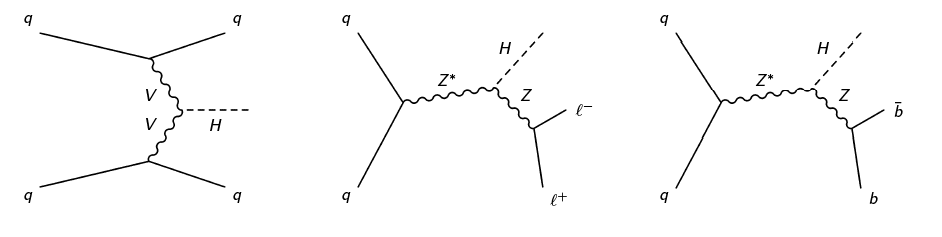
\includegraphics[width=\textwidth]{TalkPics/invcomb021213/feyndiags}
%% \begin{fmfgraph*}(100,70)
%%         \fmfleft{i1,i2}
%%         \fmfright{o1,o2,o3}
%%         \fmf{fermion}{i1,v1,o1}
%%         \fmf{fermion}{i2,v2,o3}
%%         \fmf{phantom,tension=4/5}{v1,v2}
%%         \fmffreeze
%%         \fmf{photon,label=$W,,Z$}{v1,v3}
%%         \fmf{photon,label=$W,,Z$}{v2,v3}
%%         \fmf{dashes}{v3,o2}
%%         \fmflabel{$q$}{i1}
%%         \fmflabel{$q$}{i2}
%%         \fmflabel{$q$}{o1}
%%         \fmflabel{$q$}{o3}
%%         \fmflabel{$H$}{o2}
%%       \end{fmfgraph*}
}
\date{}
\begin{document}
\begin{fmffile}{higgsexoupdatefeyndiags}

%TITLE PAGE
\section{Title}
\begin{frame}
  \titlepage
  
\end{frame}

%OUTLINE
\begin{frame}
  \frametitle{Introduction}
  \begin{block}{}
    \scriptsize
    \begin{itemize}
    \item Bug found which meant we weren't running properly over run C data:
    \item[-] meant background estimate was normalised only to part of the full luminosity
    \item Bug correction therefore increased background estimate
    \item Signal was already normalised to the full luminosity so didn't change
    \item Limit for old signal region is therefore worsened to 43\%
    \item However increased background makes old signal region no longer optimum
    \end{itemize}
  \end{block}
\end{frame}

\begin{frame}
  \frametitle{Check Data-MC - munu}
  \begin{columns}
    \column{.5\textwidth}
    \begin{block}{Jet 1 pt}
      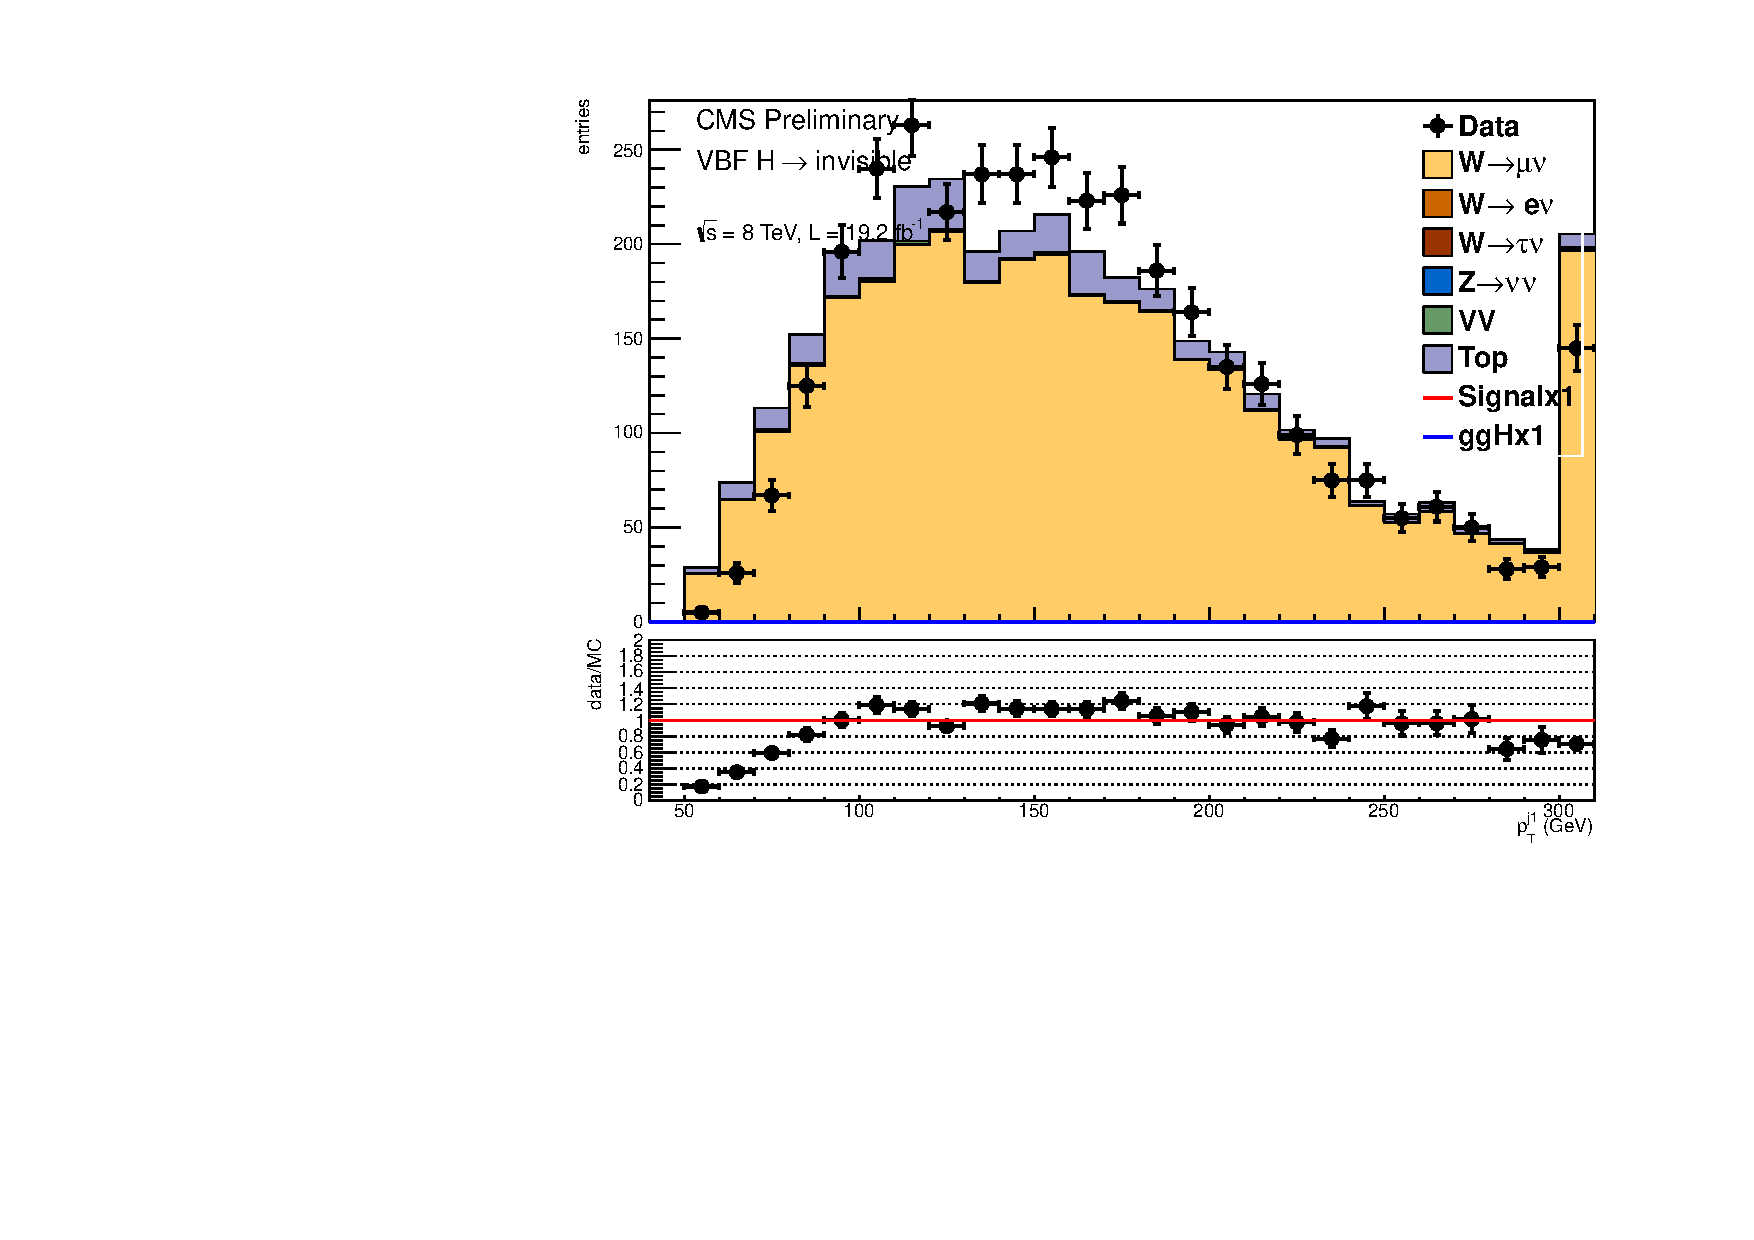
\includegraphics[width=\textwidth]{TalkPics/runcbug101114/output_presel/munu_jet1_pt.pdf}
    \end{block}
    \column{.5\textwidth}
    \begin{block}{Jet 2 pt}
      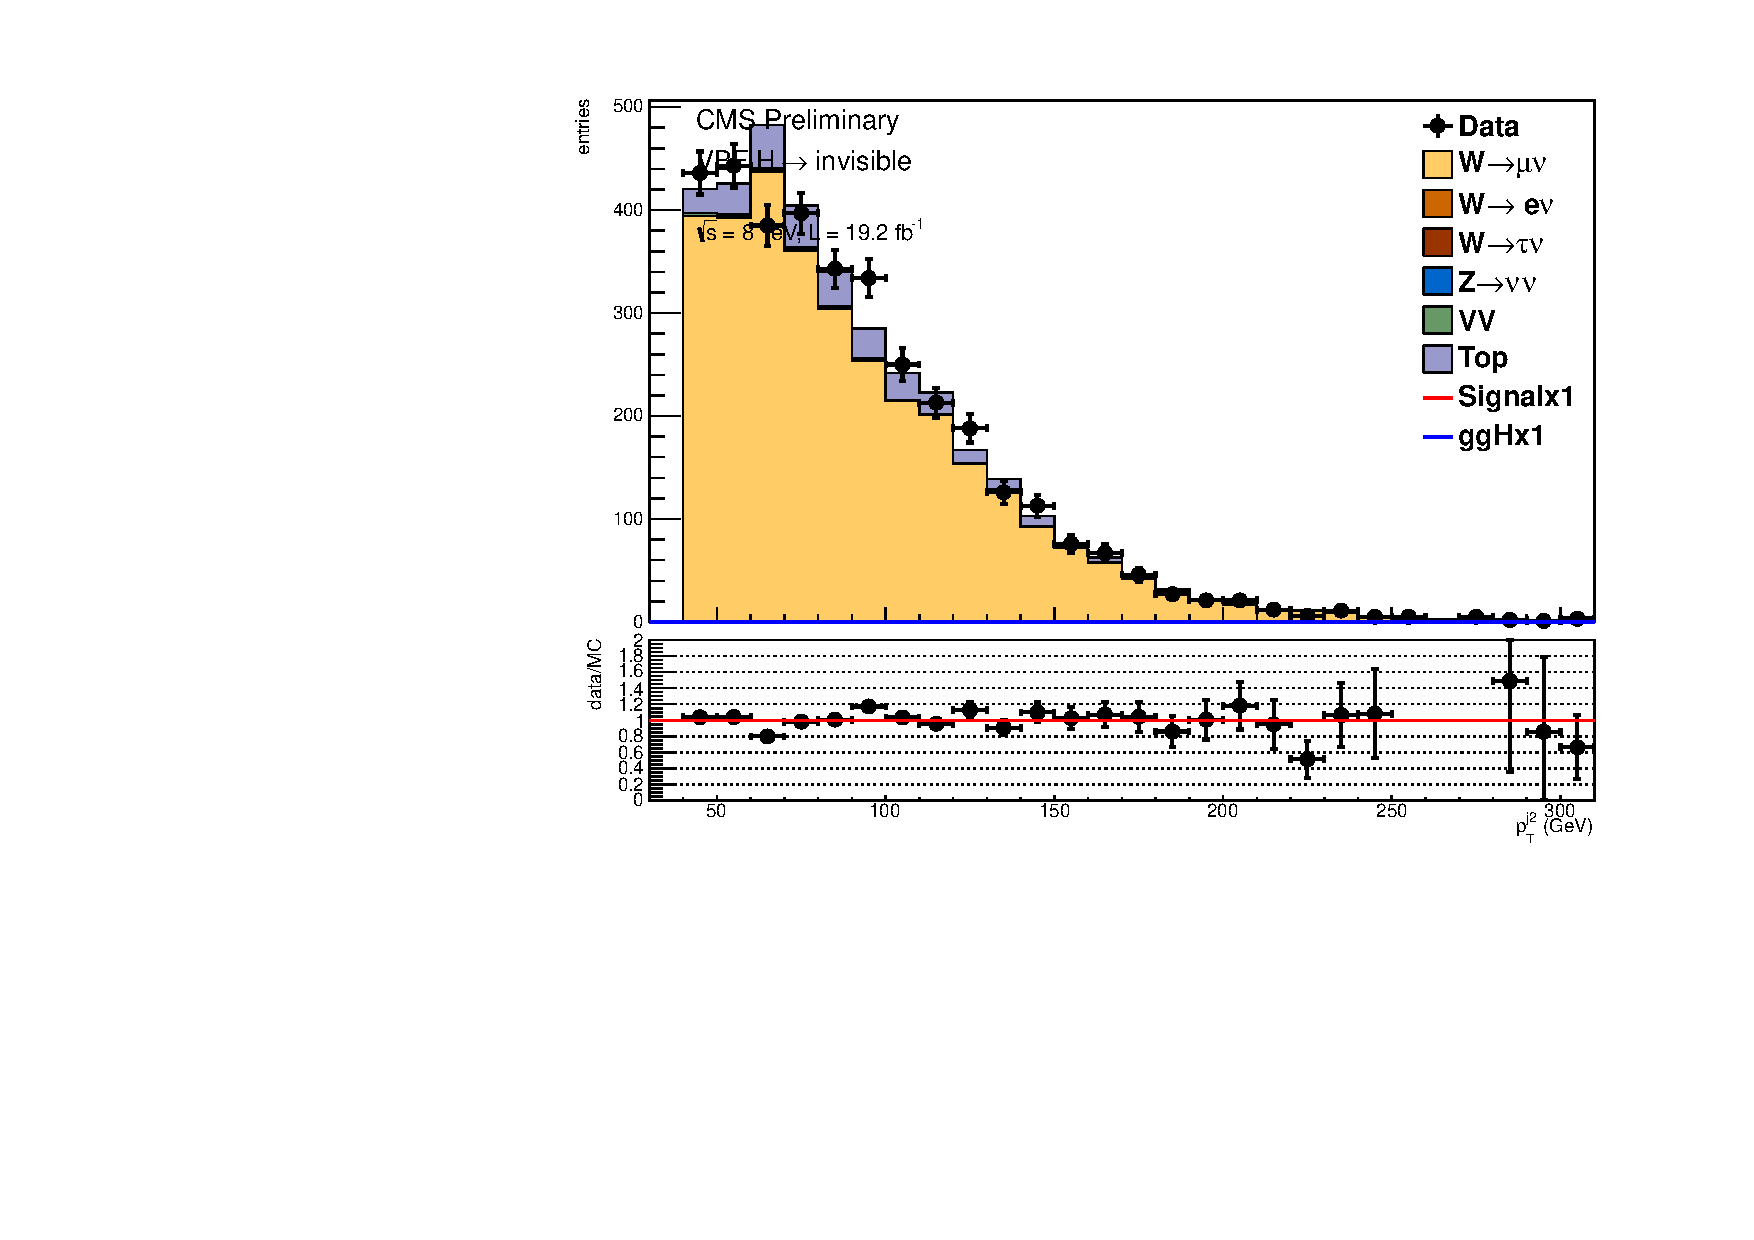
\includegraphics[width=\textwidth]{TalkPics/runcbug101114/output_presel/munu_jet2_pt.pdf}
    \end{block}

  \end{columns}
\end{frame}

\begin{frame}
  \frametitle{Check Data-MC - munu}
  \begin{columns}
    \column{.5\textwidth}
    \begin{block}{METnomu}
      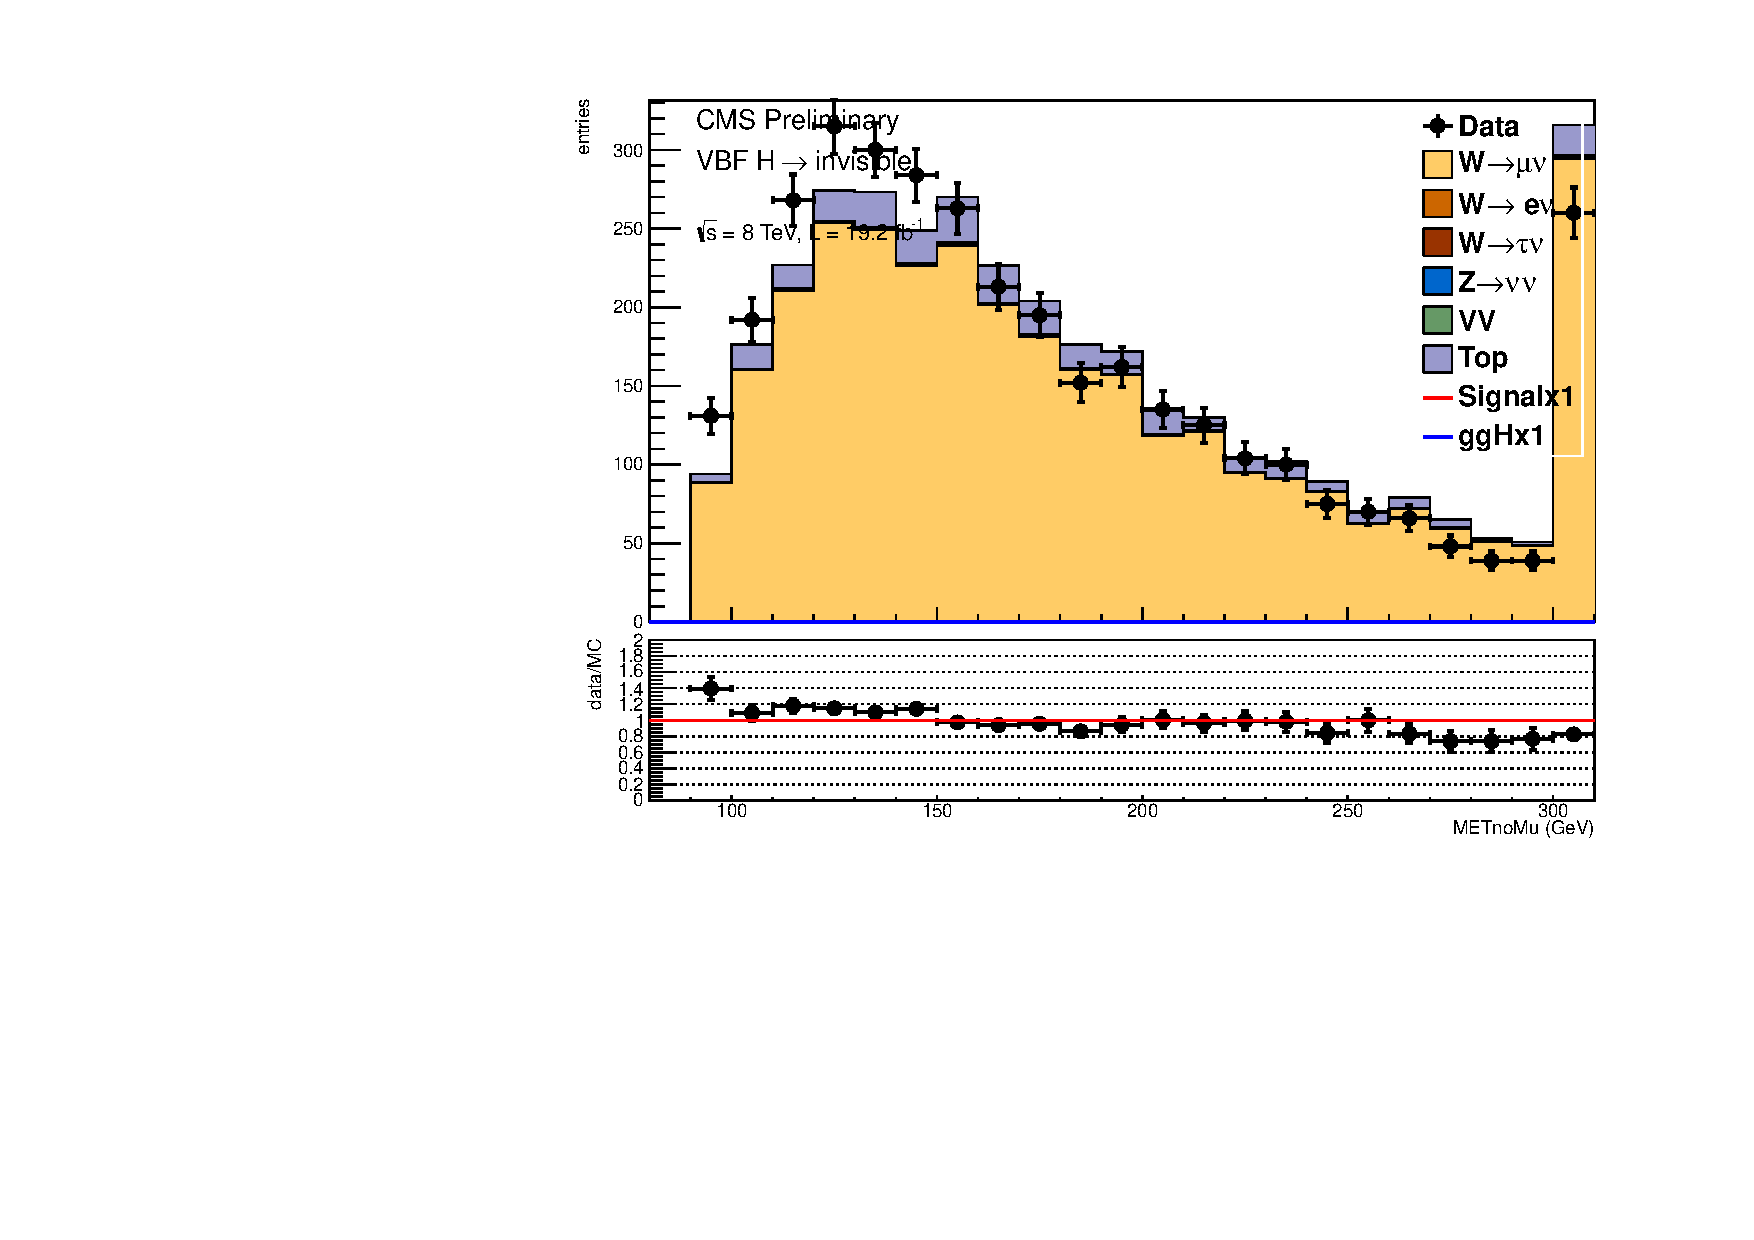
\includegraphics[width=\textwidth]{TalkPics/runcbug101114/output_presel/munu_metnomuons.pdf}
    \end{block}
    \column{.5\textwidth}
    \begin{block}{METnomusig}
      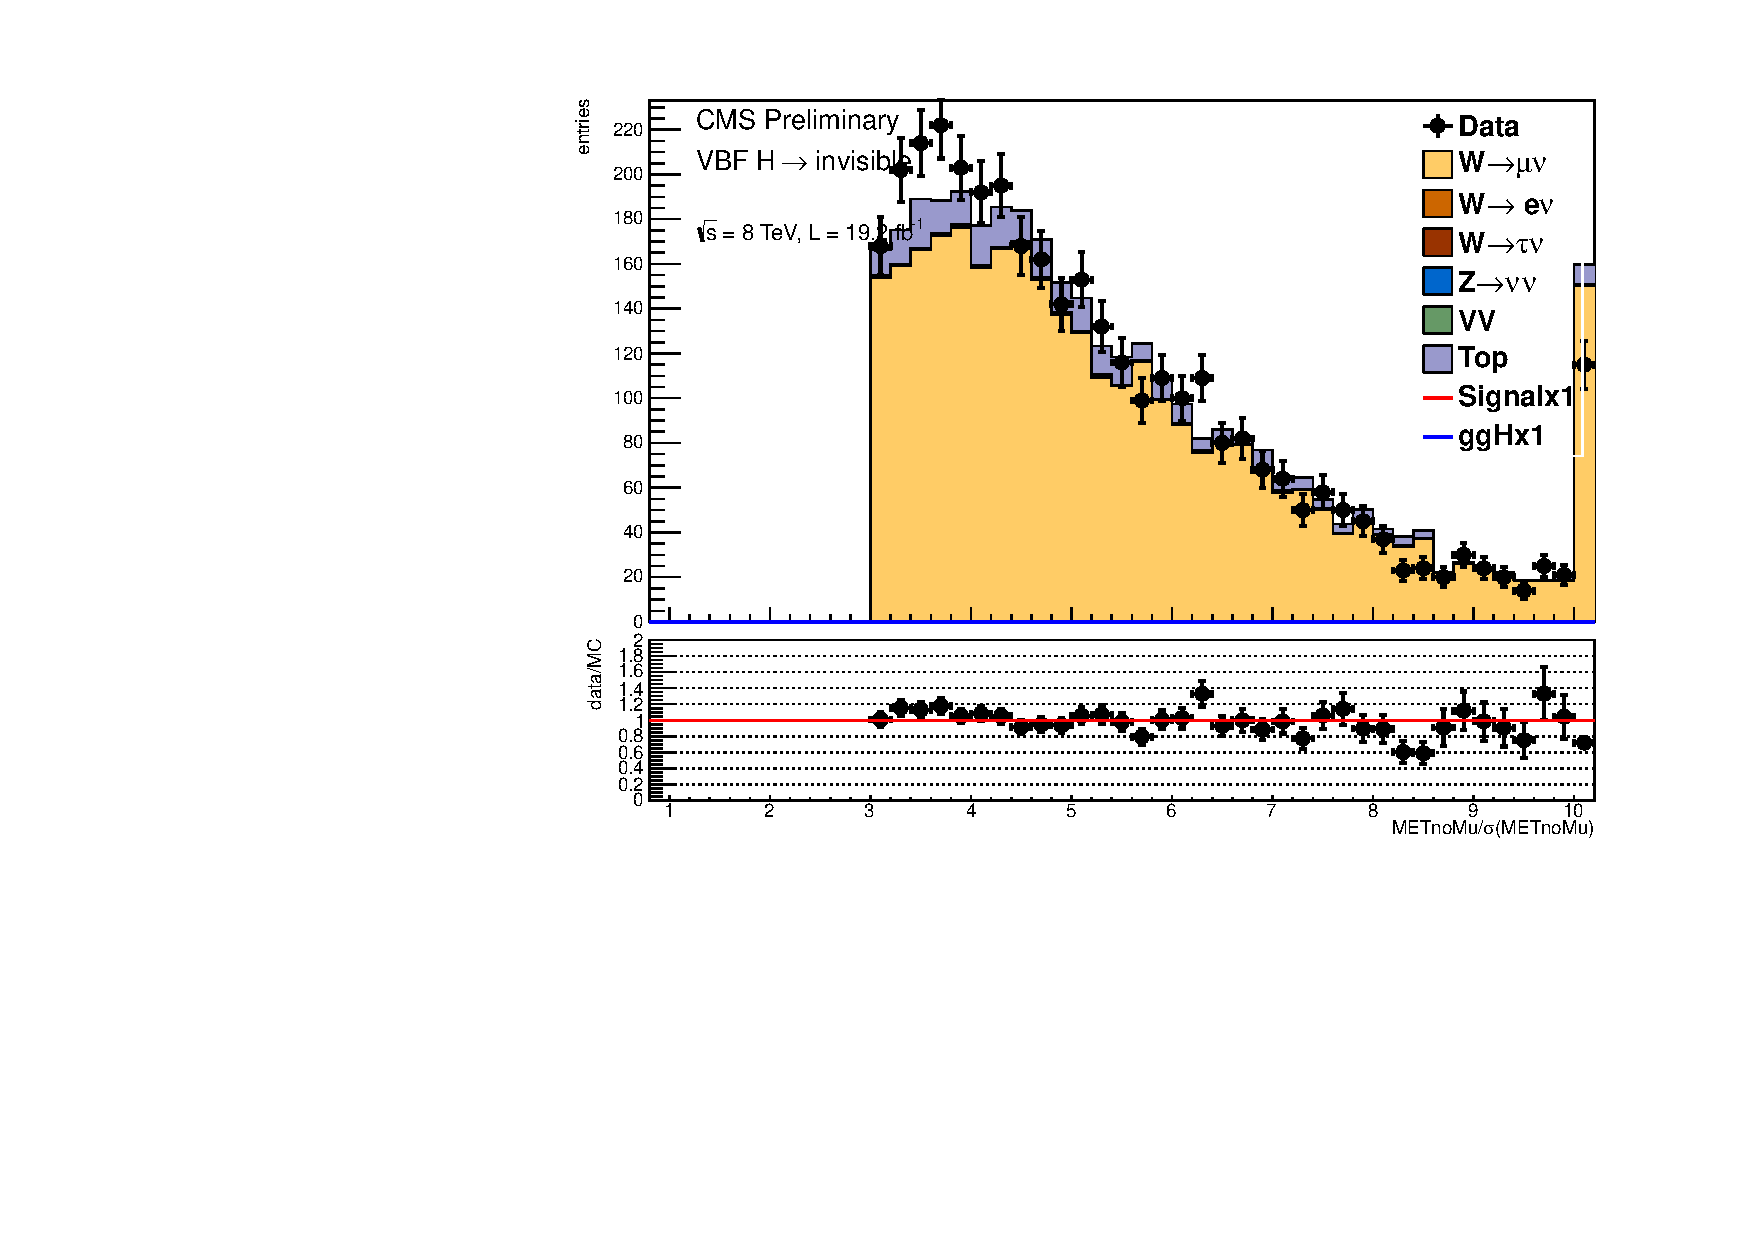
\includegraphics[width=\textwidth]{TalkPics/runcbug101114/output_presel/munu_metnomu_significance.pdf}
    \end{block}

  \end{columns}
\end{frame}

\begin{frame}
  \frametitle{Check Data-MC - munu}
  \begin{columns}
    \column{.5\textwidth}
    \begin{block}{Mjj}
      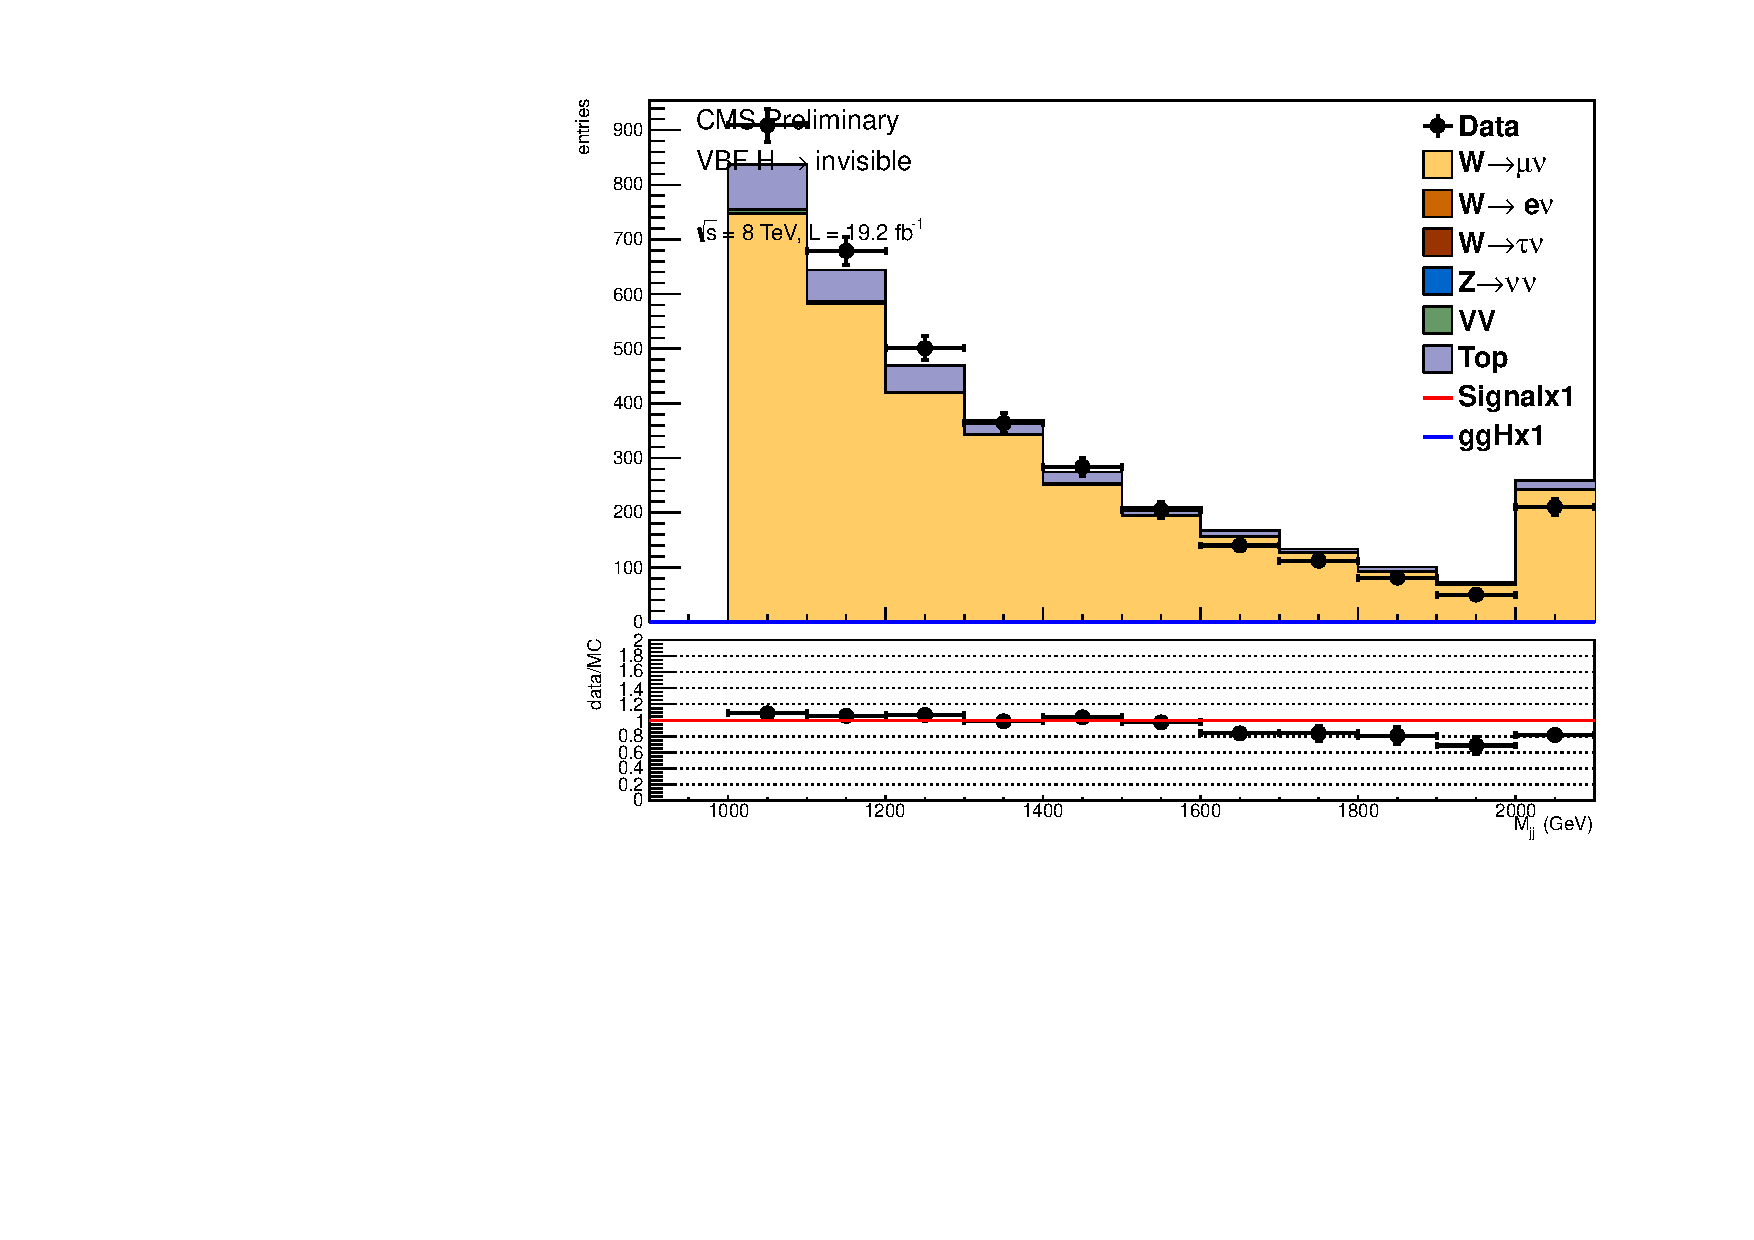
\includegraphics[width=\textwidth]{TalkPics/runcbug101114/output_presel/munu_dijet_M.pdf}
    \end{block}
    \column{.5\textwidth}
    \begin{block}{mt}
      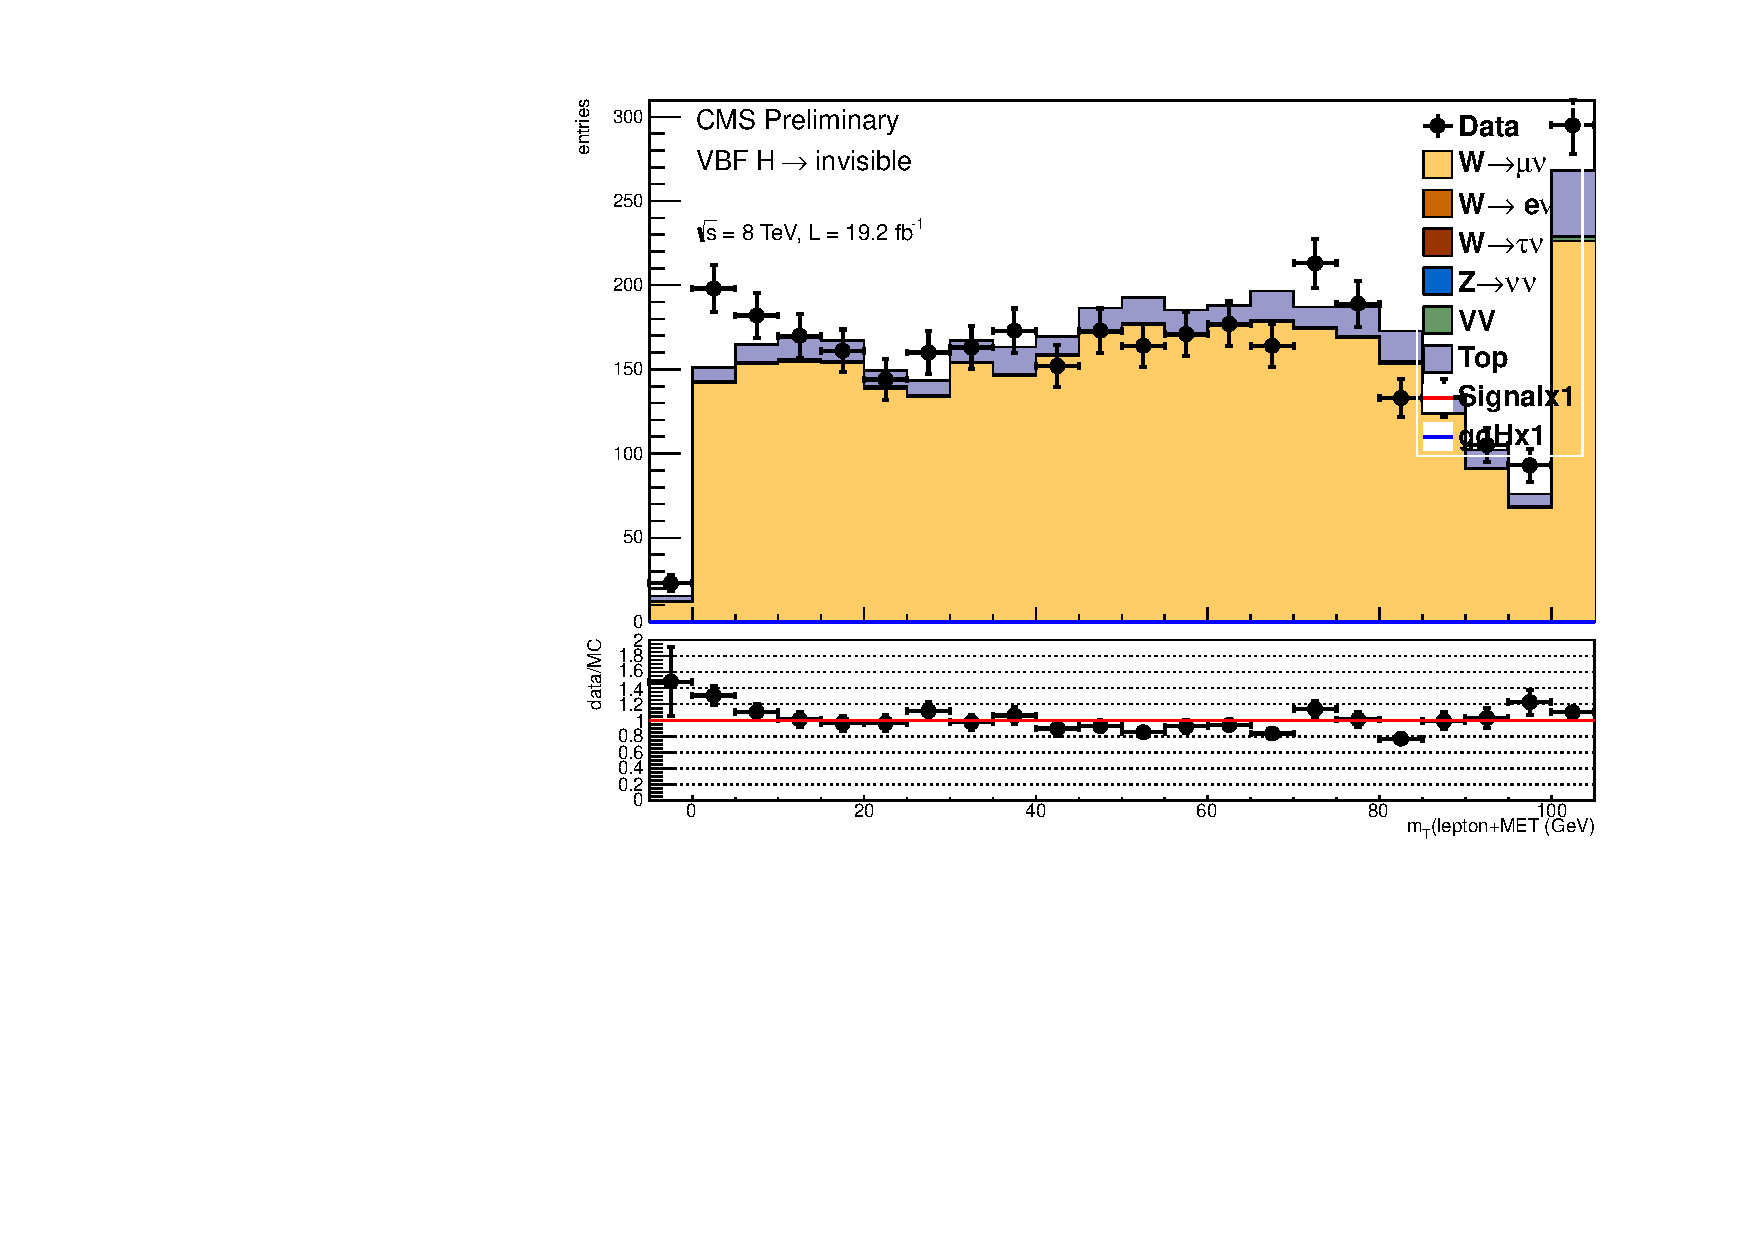
\includegraphics[width=\textwidth]{TalkPics/runcbug101114/output_presel/munu_lep_mt.pdf}
    \end{block}
  \end{columns}
\end{frame}

\begin{frame}
  \frametitle{Check Data-MC - munu}
  \begin{columns}
    \column{.5\textwidth}
    \begin{block}{Dijet Dphi}
      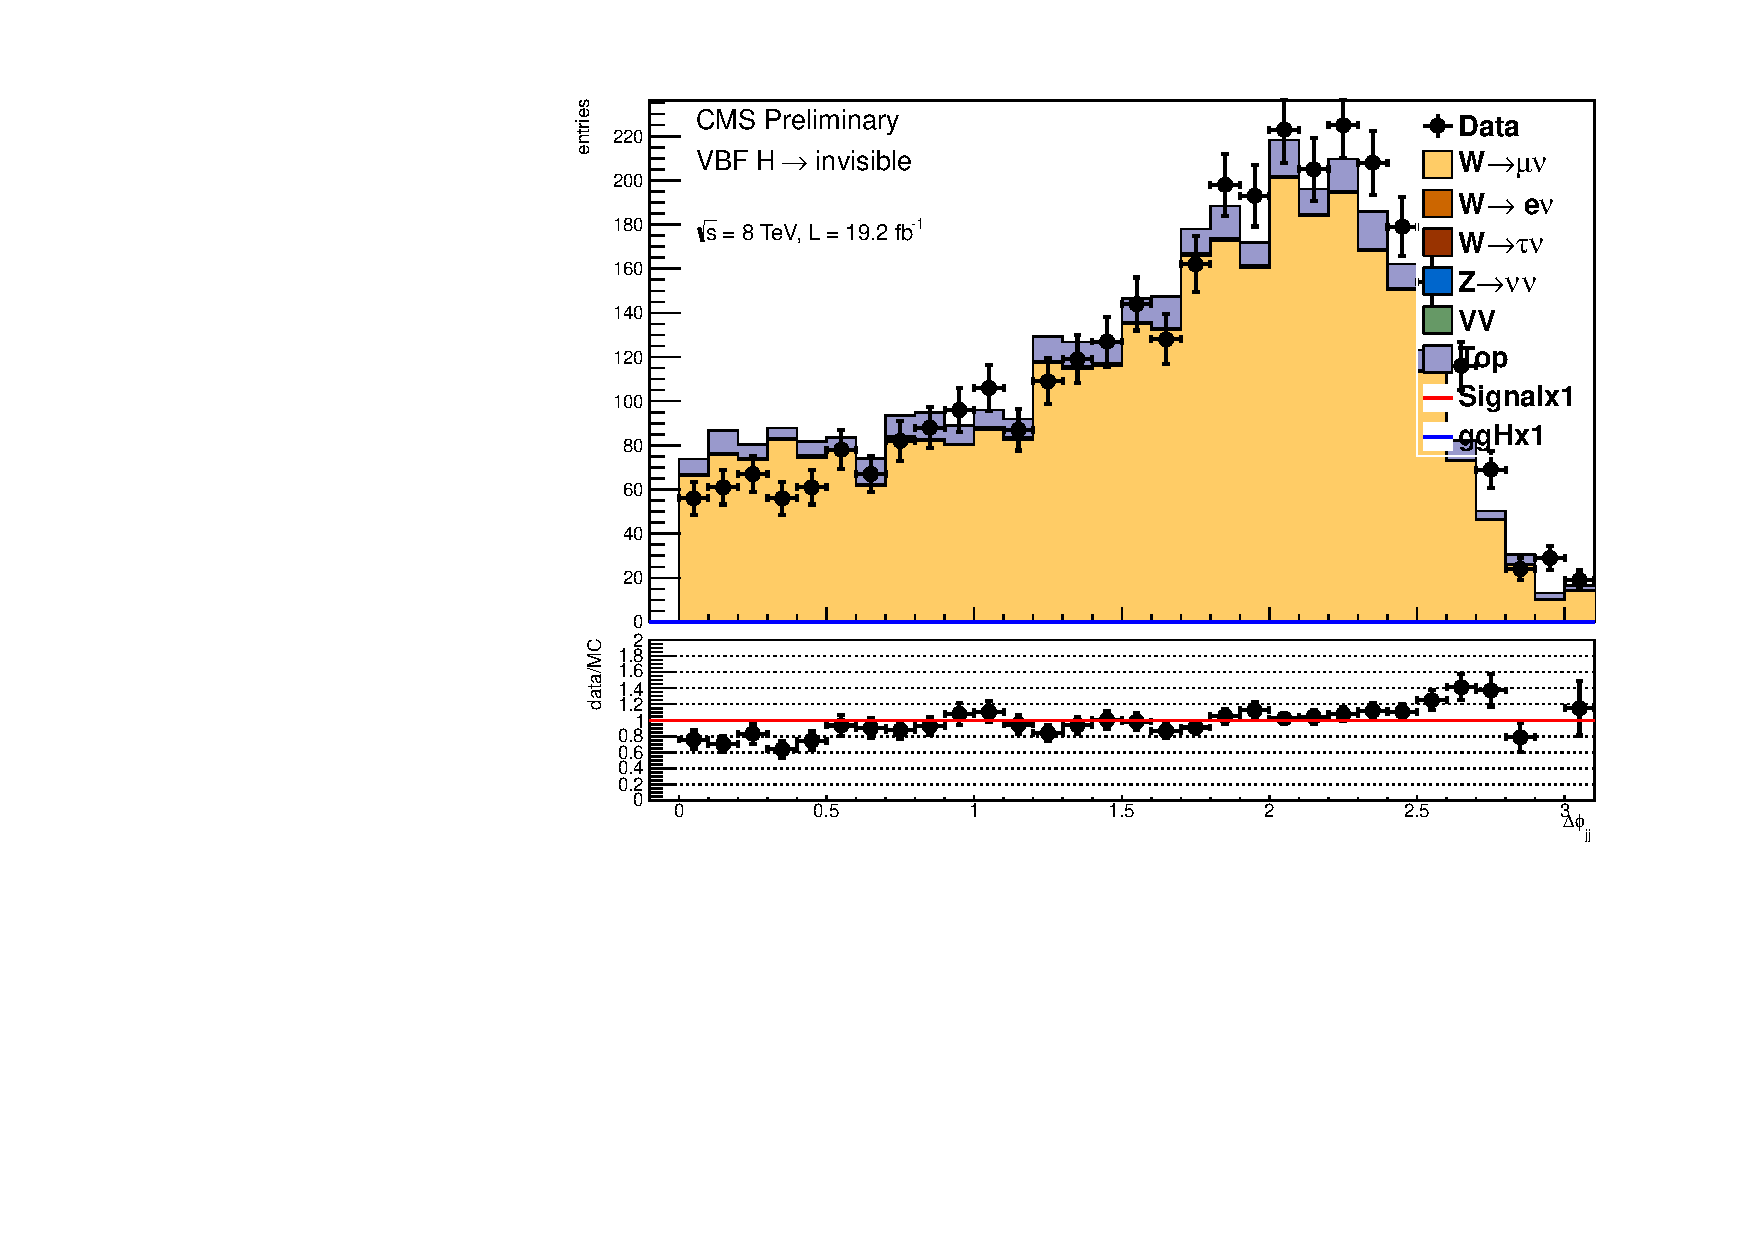
\includegraphics[width=\textwidth]{TalkPics/runcbug101114/output_presel/munu_dijet_dphi.pdf}
    \end{block}
    \column{.5\textwidth}
    \begin{block}{Detajj}
      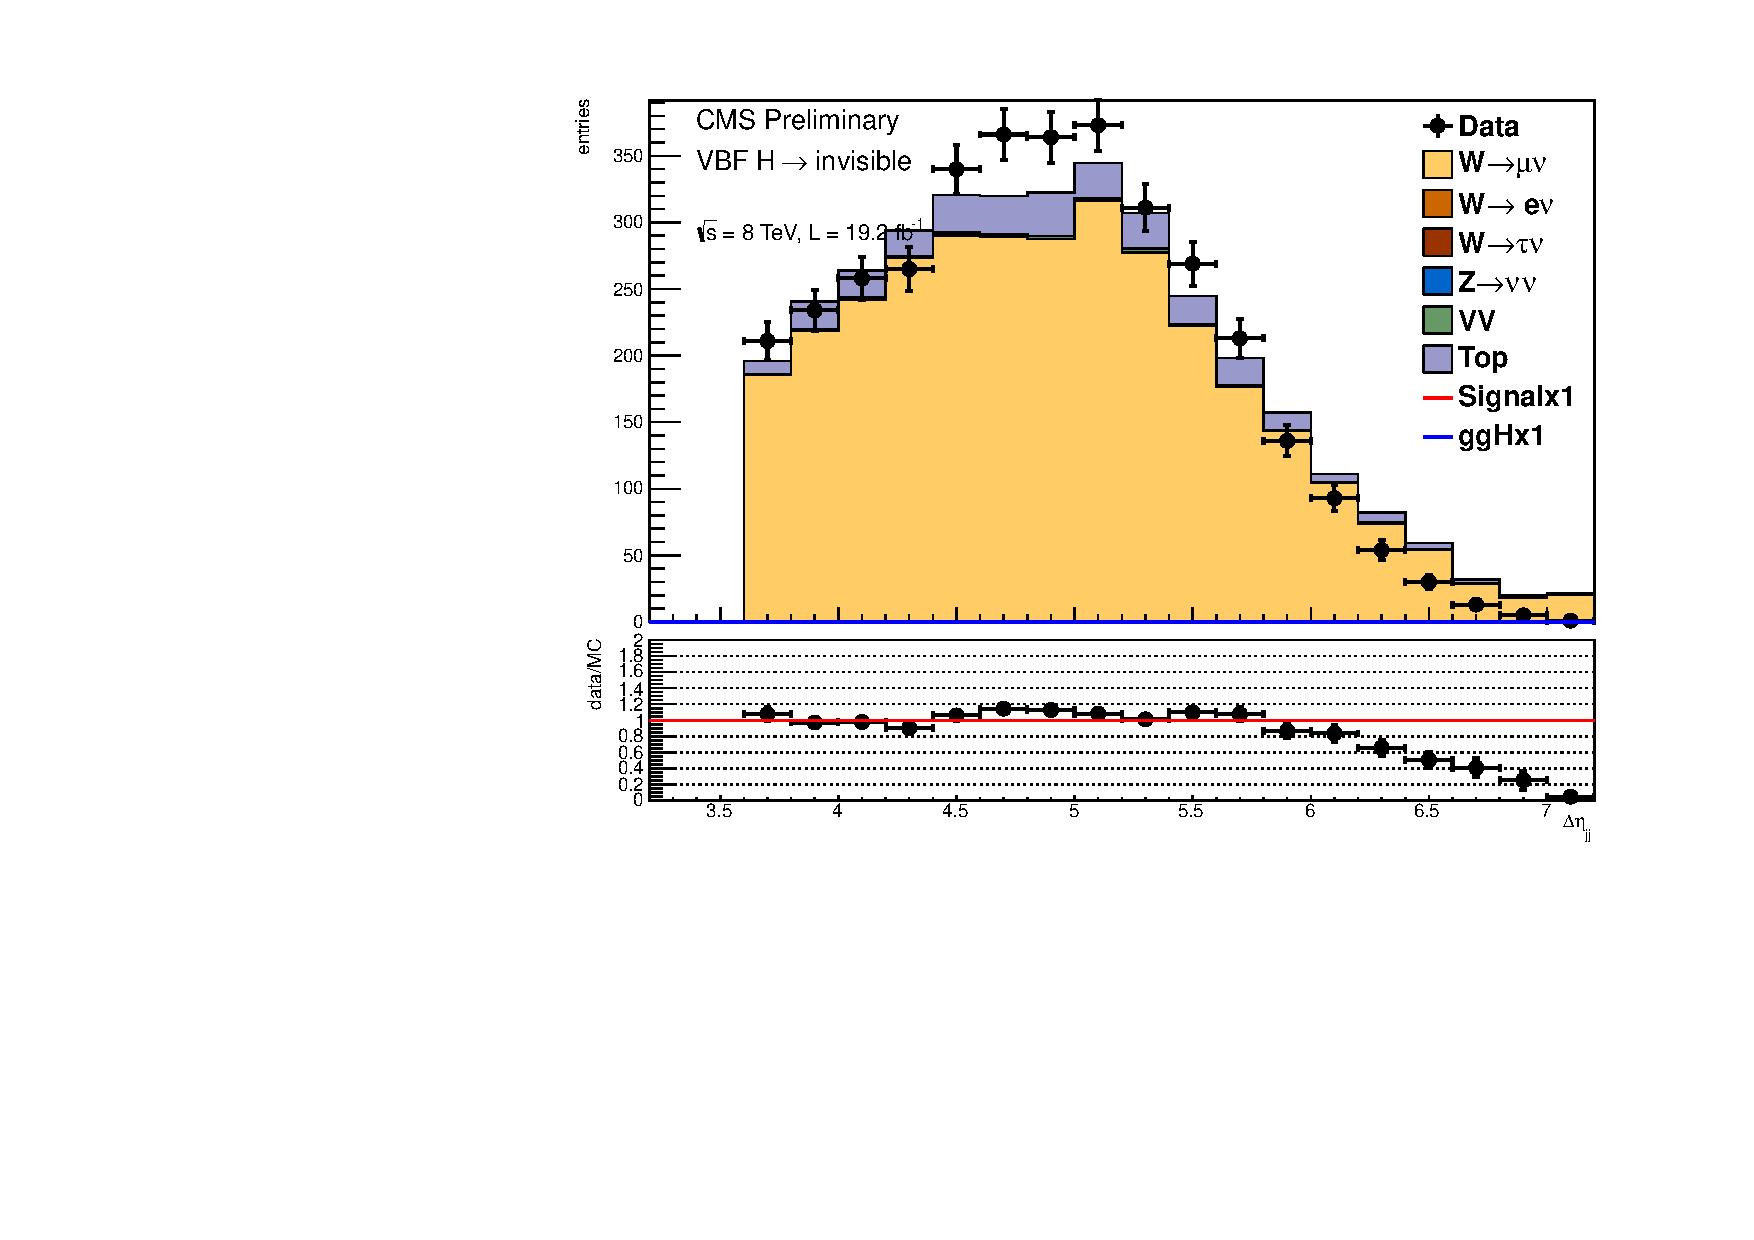
\includegraphics[width=\textwidth]{TalkPics/runcbug101114/output_presel/munu_dijet_deta.pdf}
    \end{block}

  \end{columns}
\end{frame}

\begin{frame}
  \frametitle{Check Data-MC - munu}
  \begin{columns}
    \column{.5\textwidth}
    \begin{block}{Leading jets-met mindphi}
      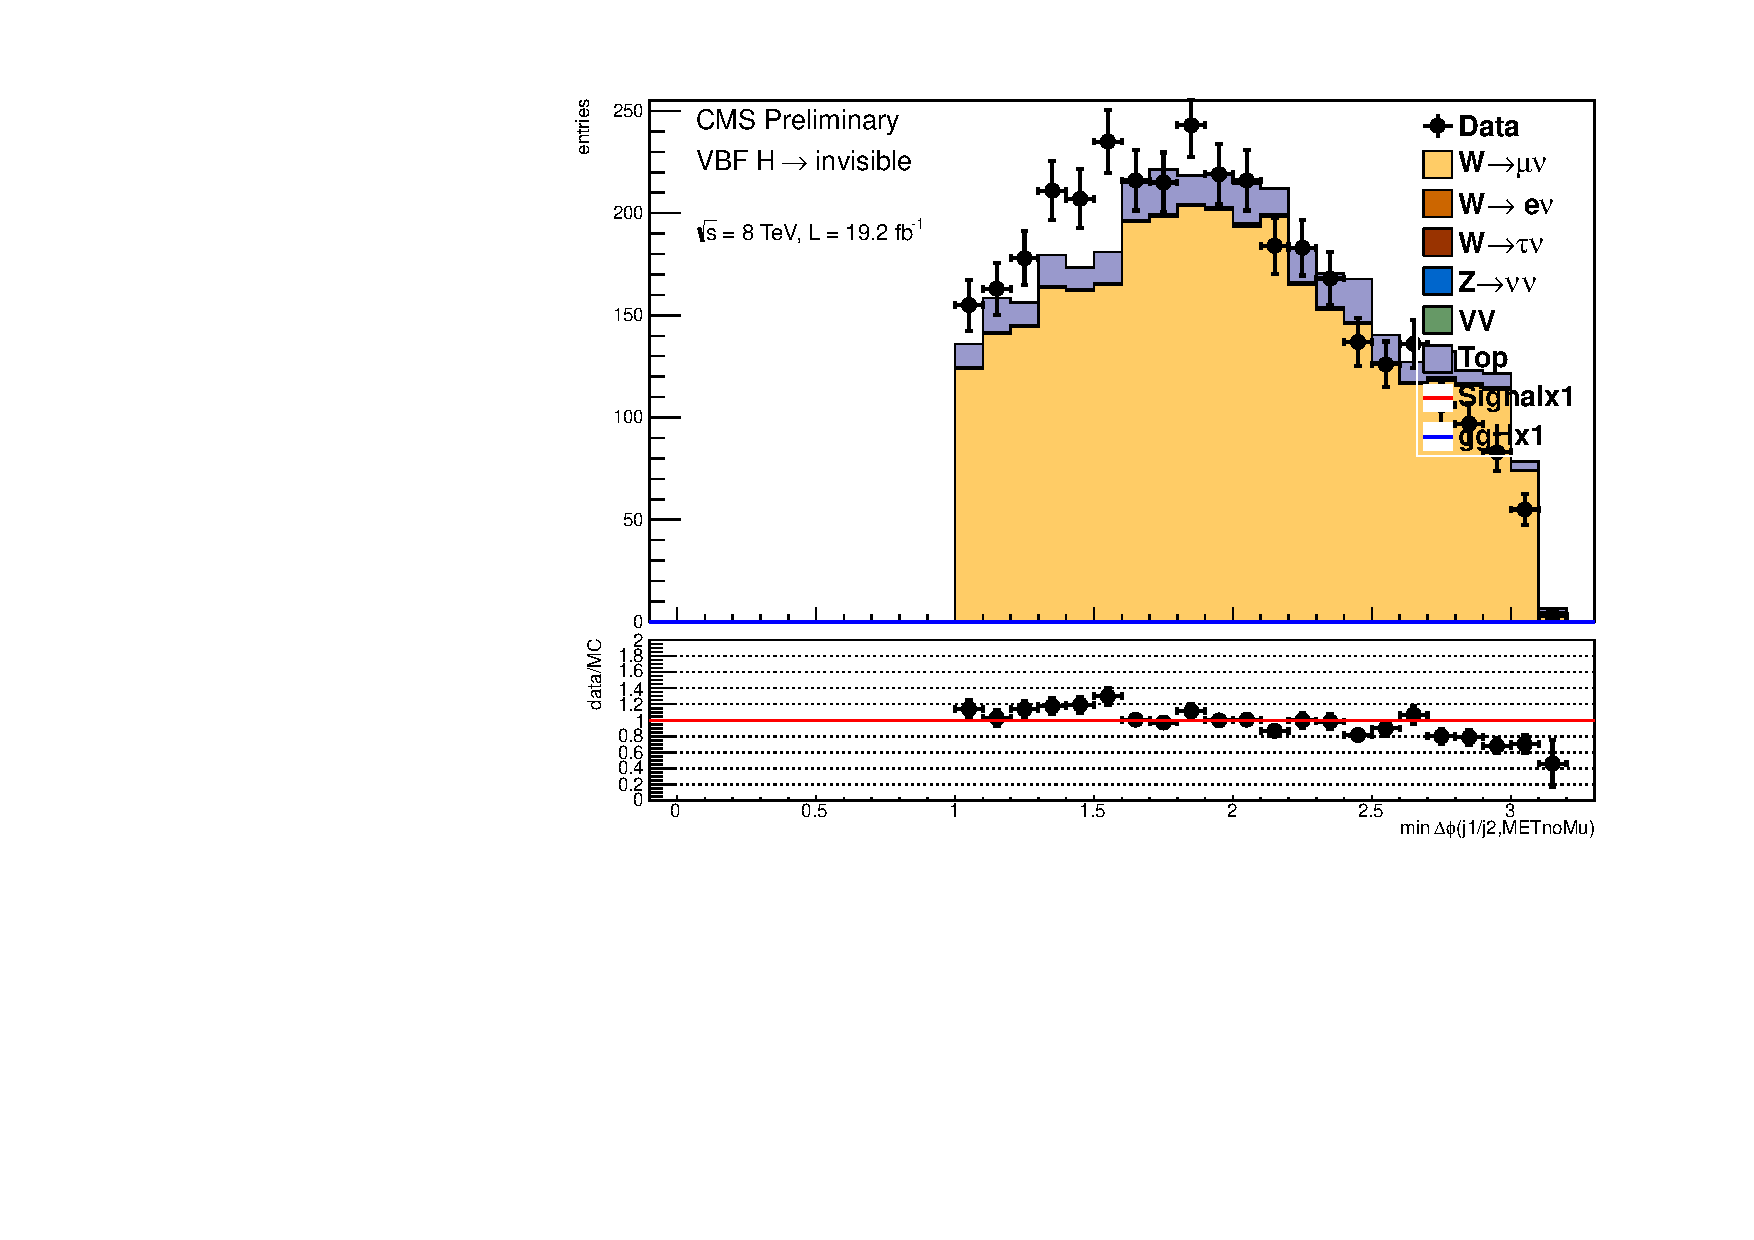
\includegraphics[width=\textwidth]{TalkPics/runcbug101114/output_presel/munu_jetmetnomu_mindphi.pdf}
    \end{block}
    \column{.5\textwidth}
    \begin{block}{All jets-met mindphi}
      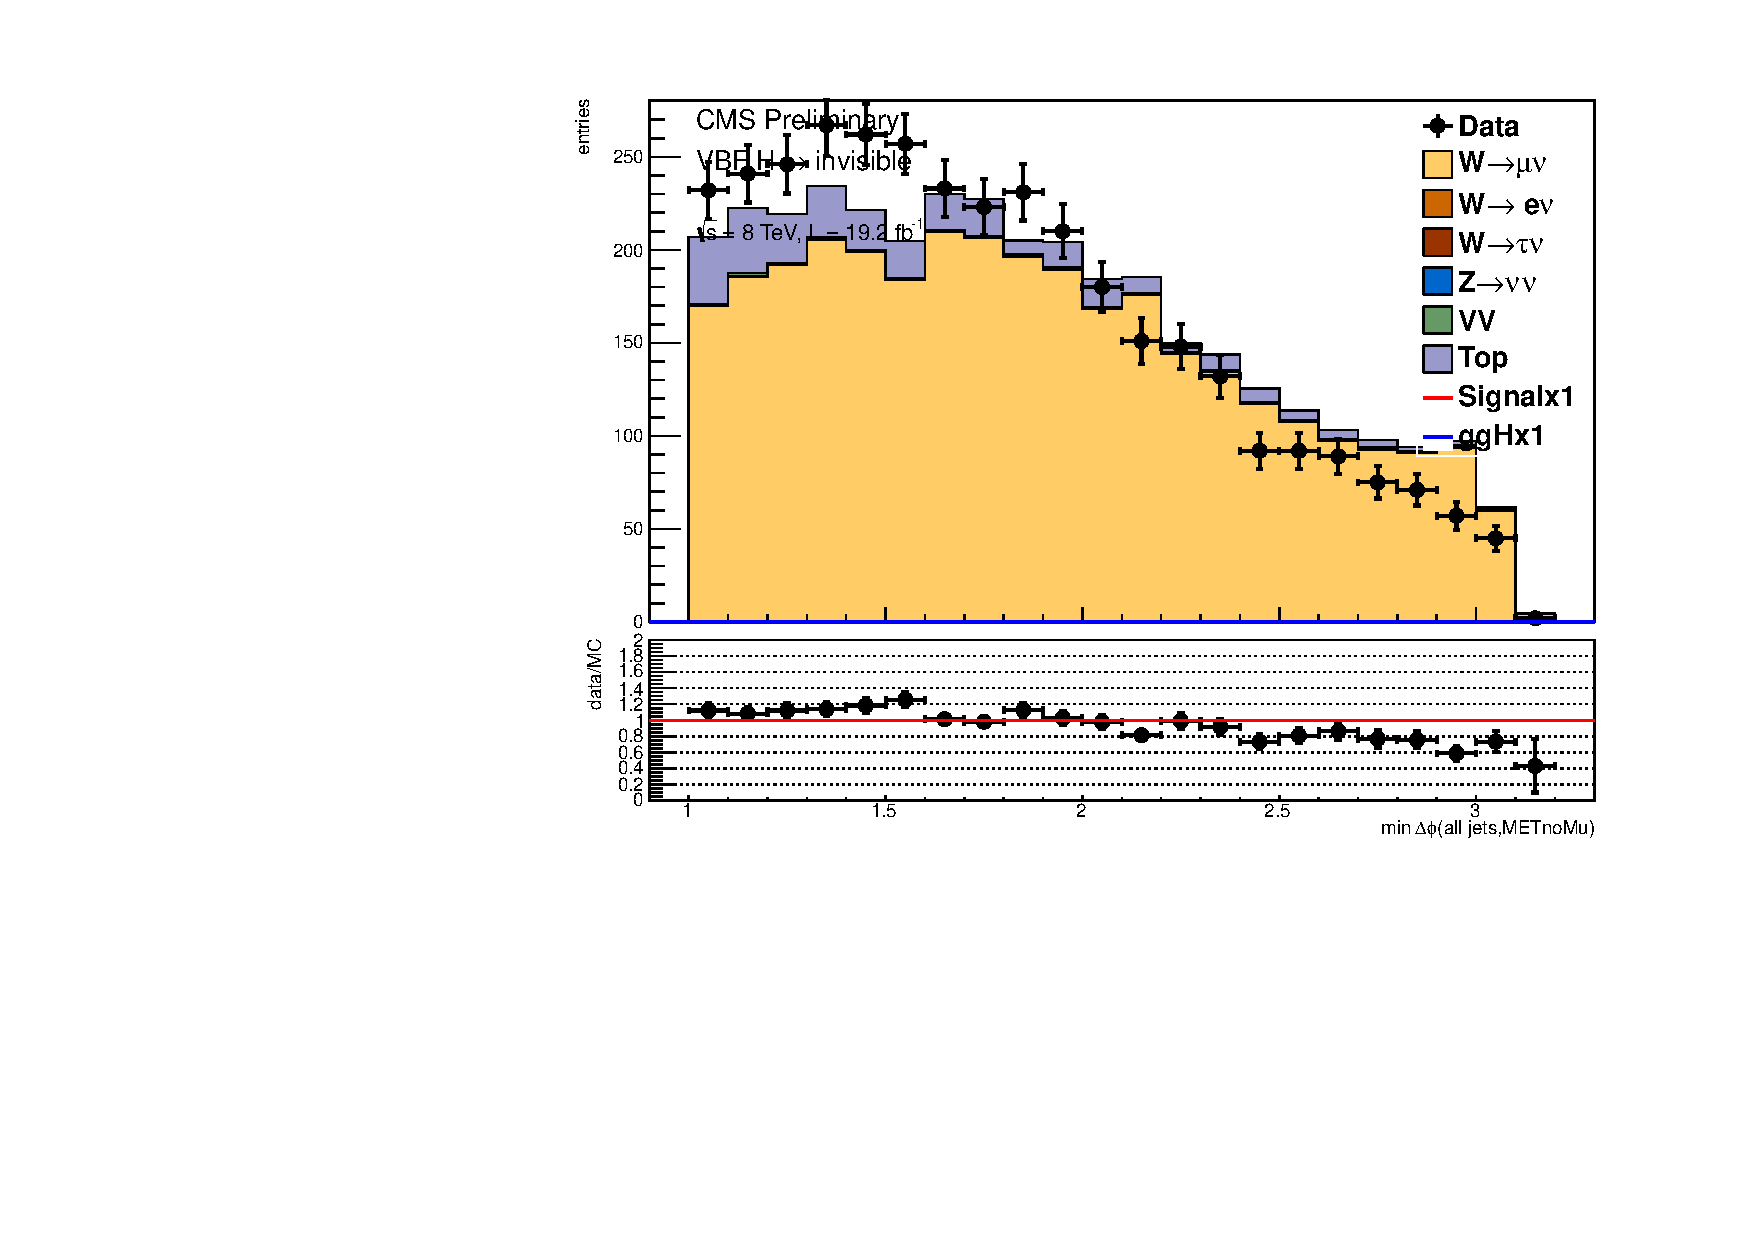
\includegraphics[width=\textwidth]{TalkPics/runcbug101114/output_presel/munu_alljetsmetnomu_mindphi.pdf}
    \end{block}

  \end{columns}
\end{frame}

\begin{frame}
  \frametitle{Check Data-MC - munu}
  \begin{columns}
    \column{.5\textwidth}
    \begin{block}{dijet-metnomu pt fraction}
      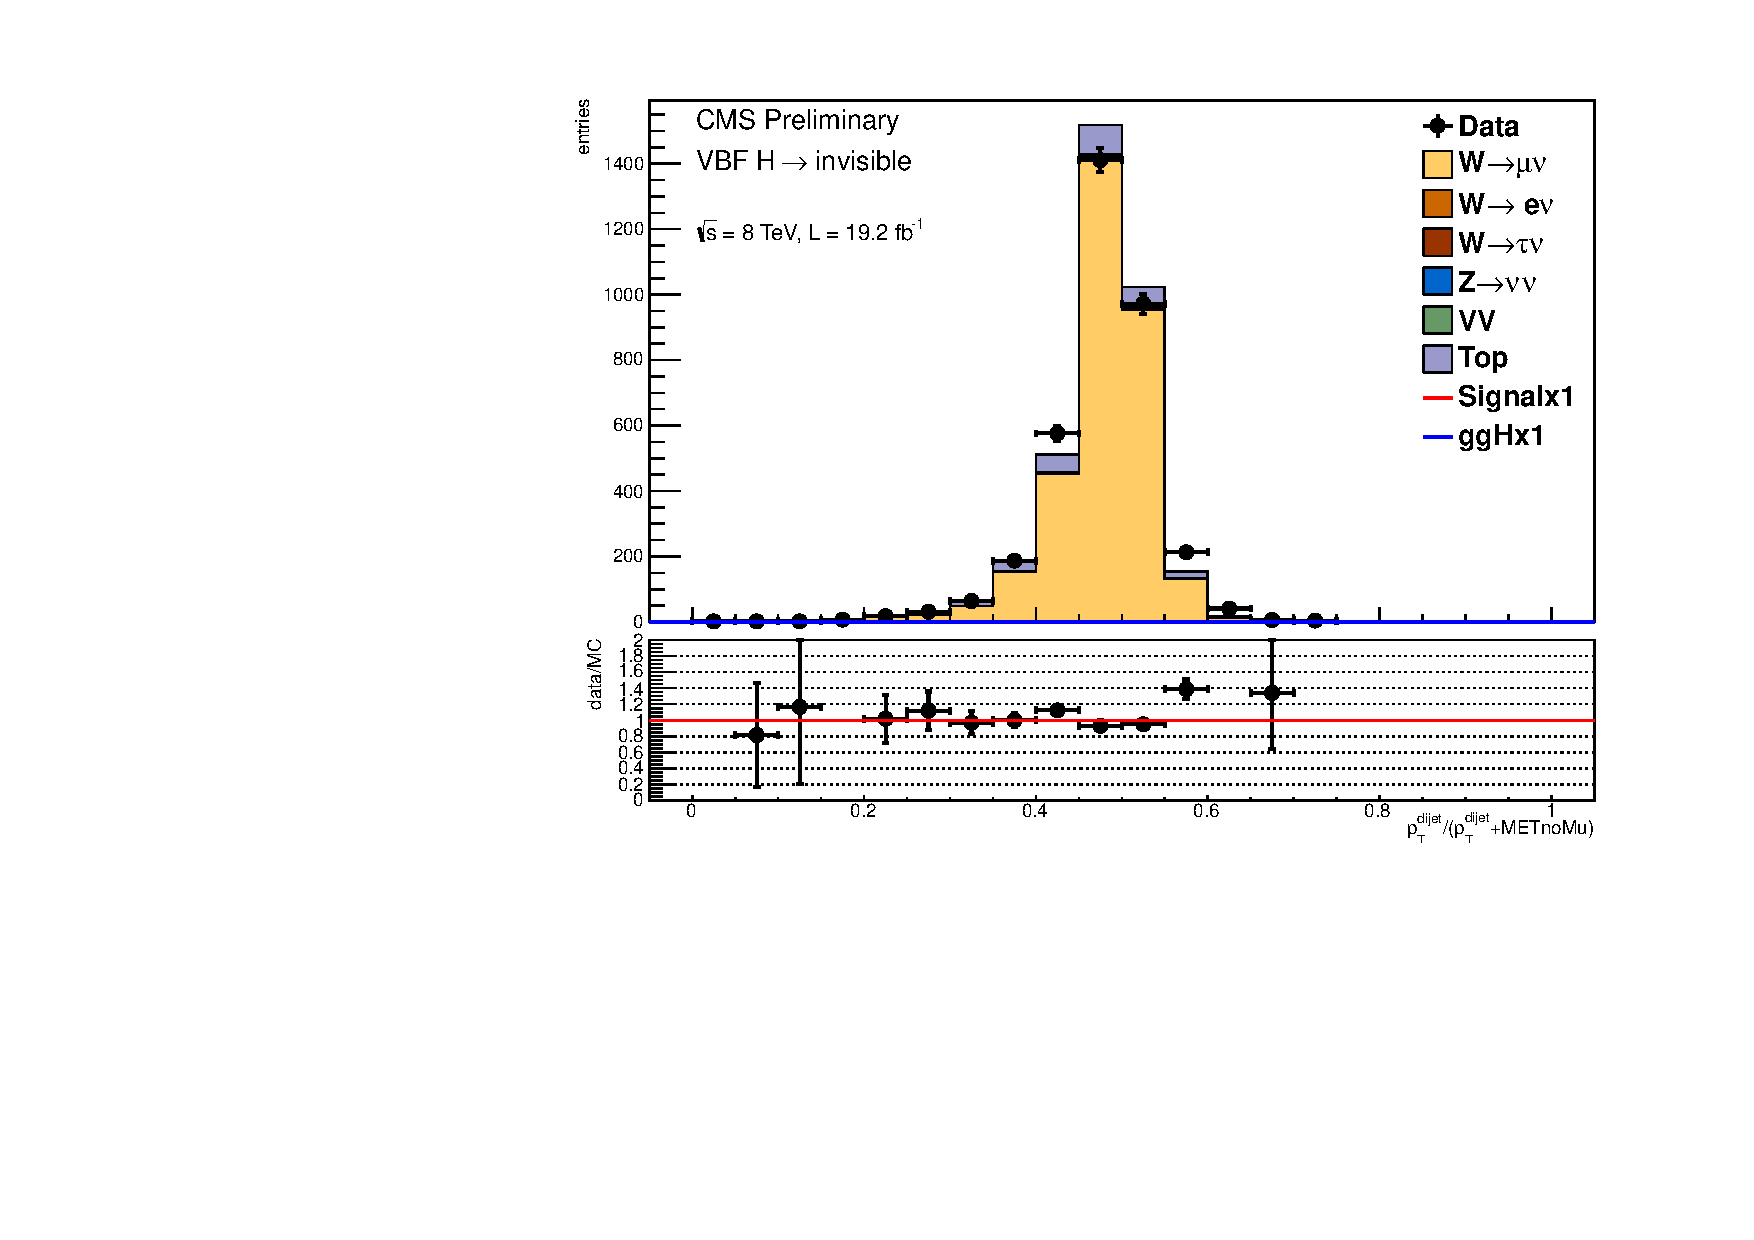
\includegraphics[width=\textwidth]{TalkPics/runcbug101114/output_presel/munu_dijetmetnomu_ptfraction.pdf}
    \end{block}
  \end{columns}
\end{frame}

\begin{frame}
  \frametitle{Check Data-MC -signal}
     \begin{columns}
       \column{1.1\textwidth}
    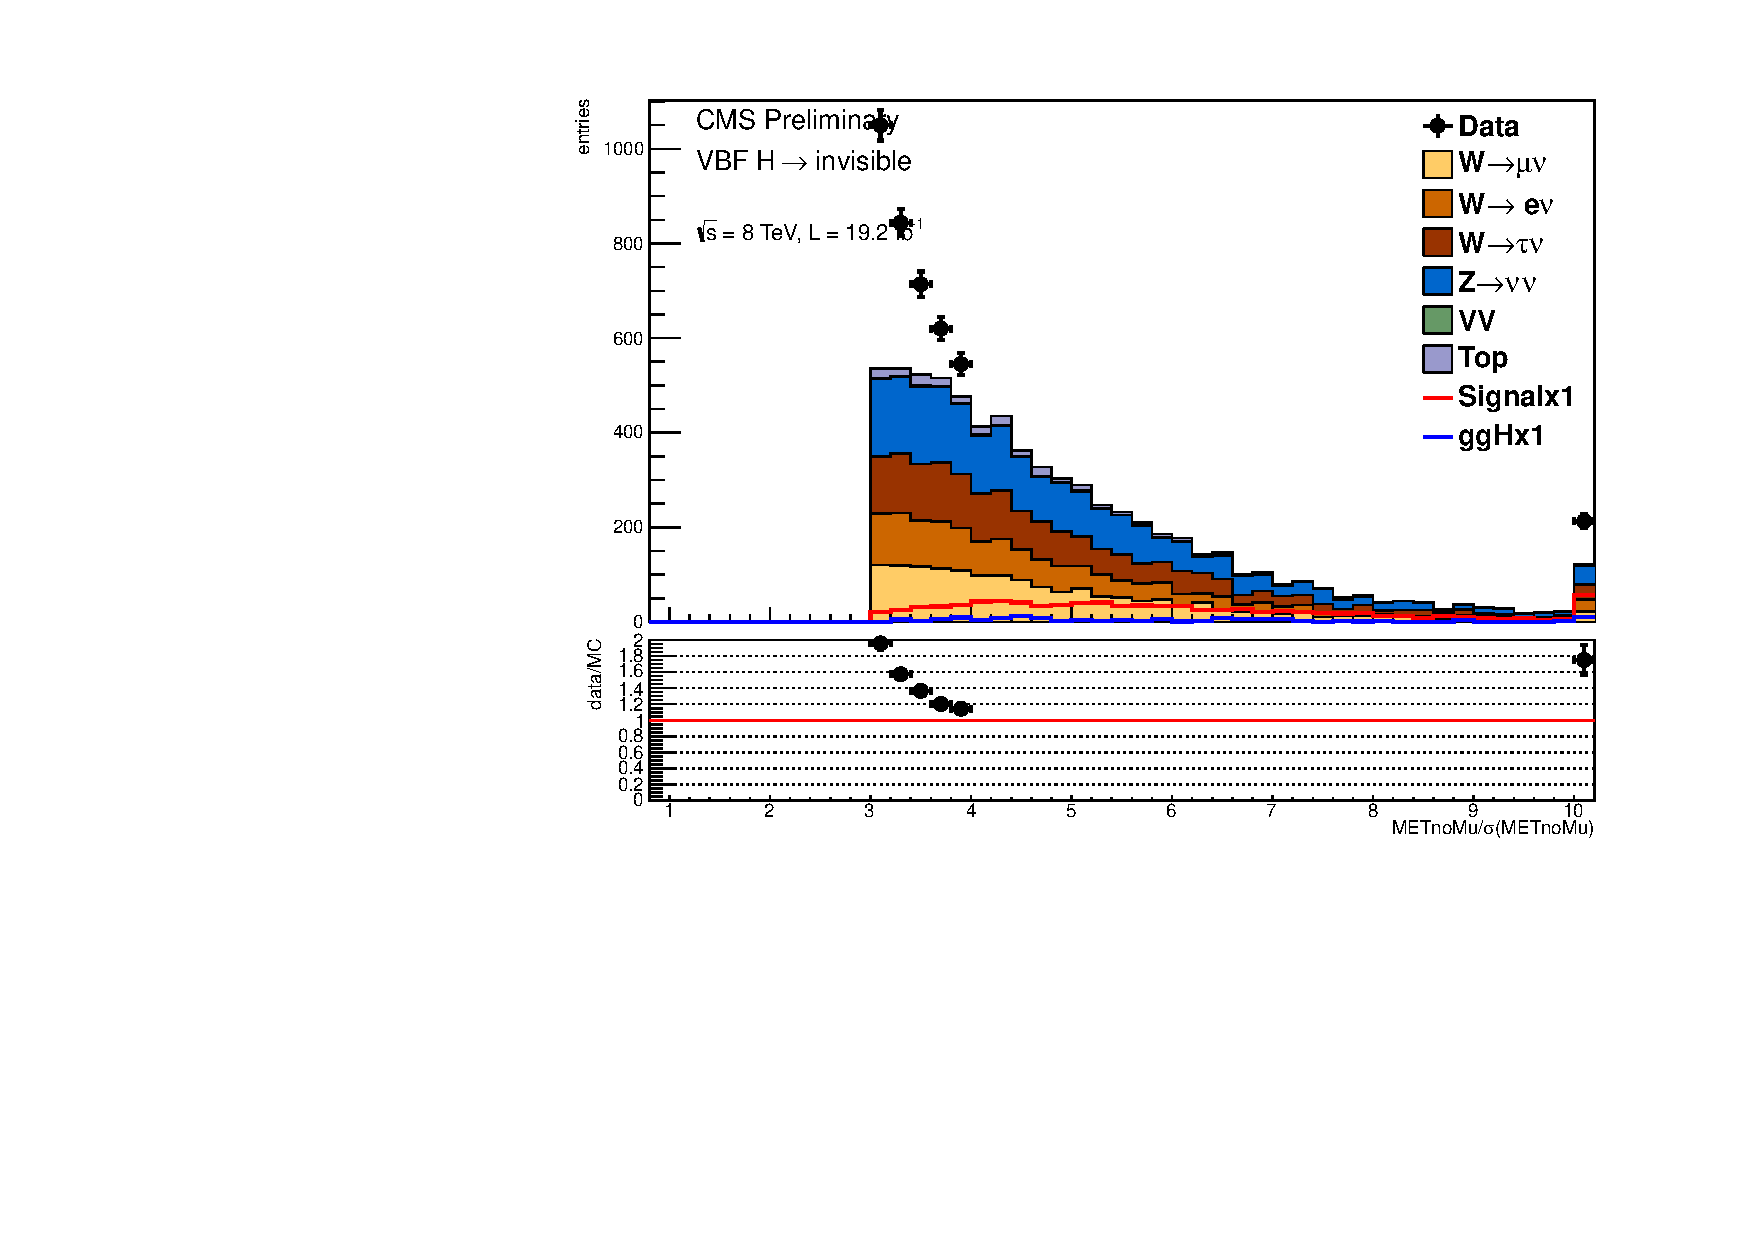
\includegraphics[clip=true,trim=0 0 0 20,width=.52\textwidth]{TalkPics/runcbug101114/output_presel/nunu_metnomu_significance.pdf}
    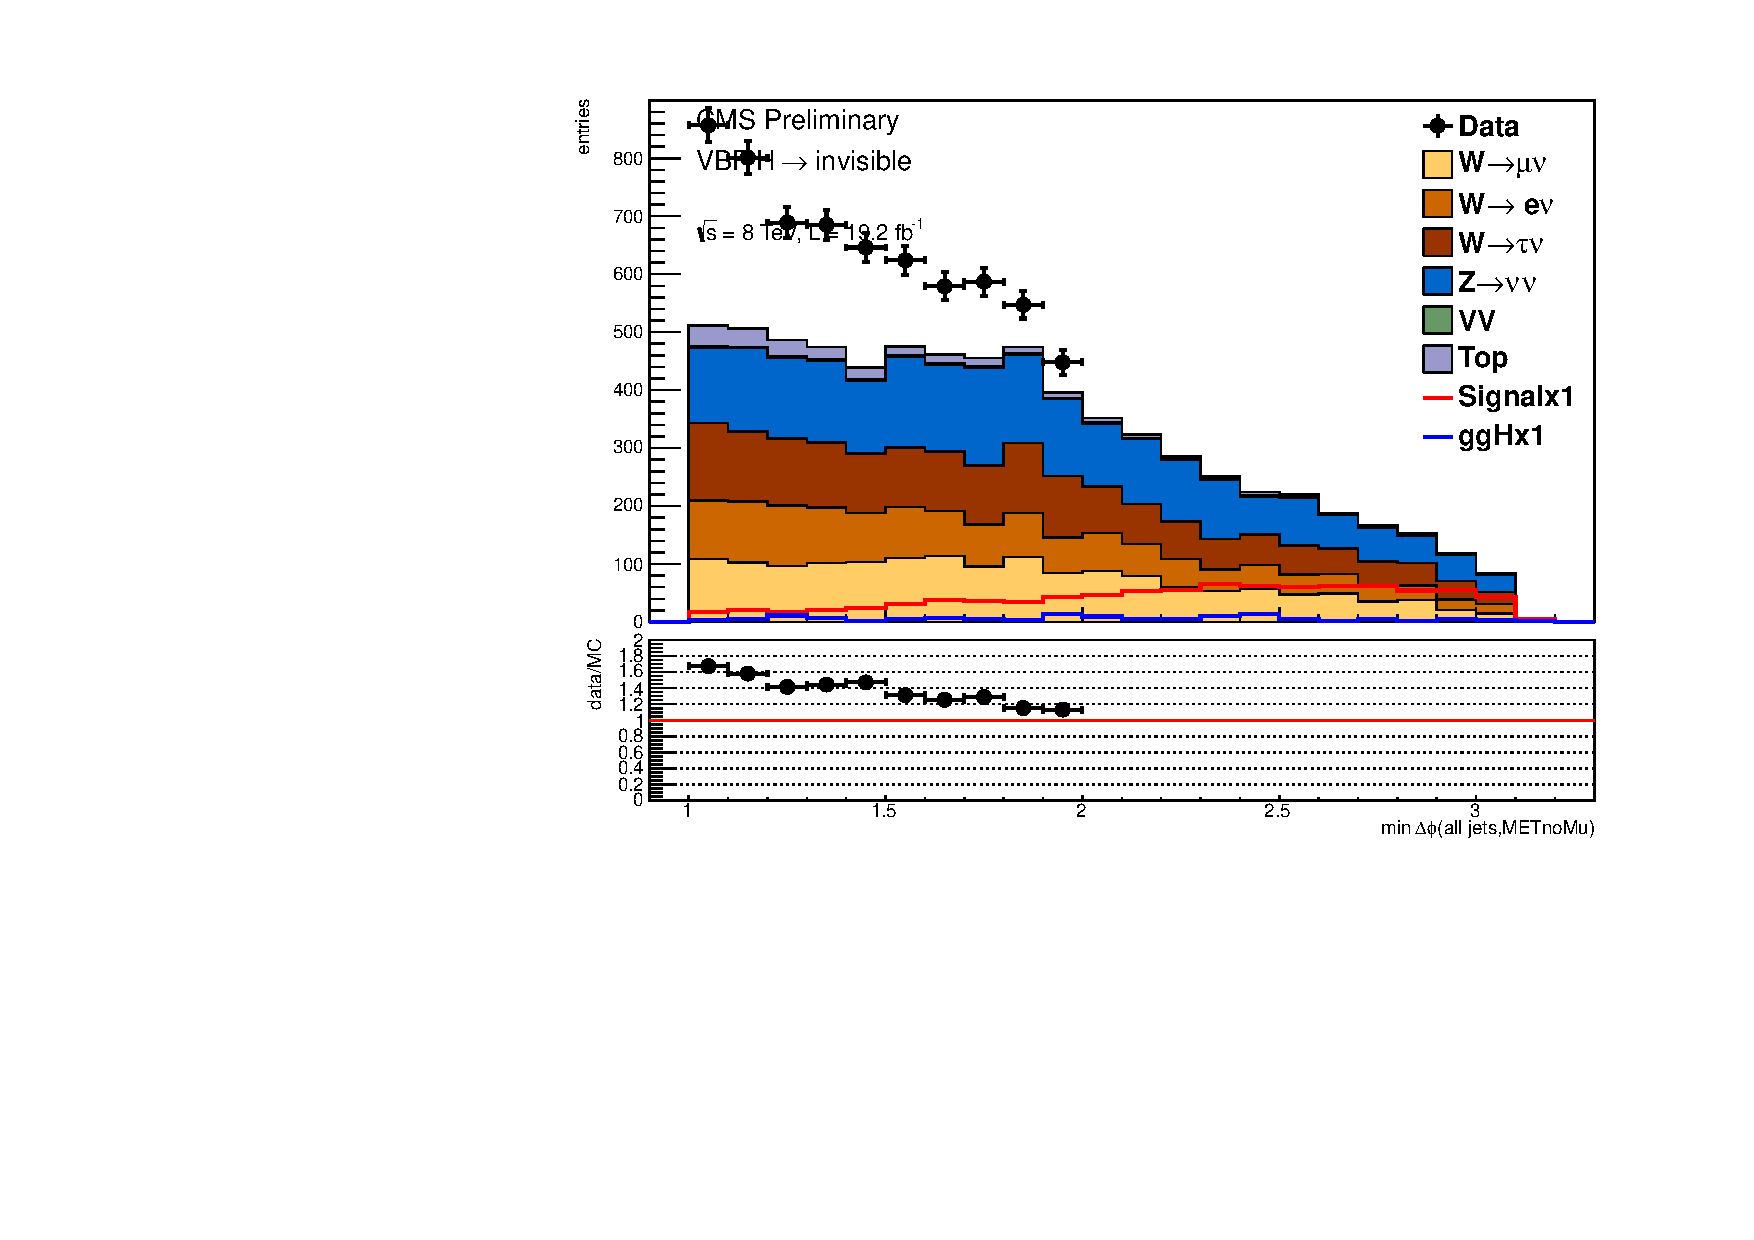
\includegraphics[clip=true,trim=0 0 0 20,width=.52\textwidth]{TalkPics/runcbug101114/output_presel/nunu_alljetsmetnomu_mindphi.pdf}
     \end{columns}
\end{frame}

\begin{frame}
  \frametitle{Signal region selection}
  \begin{block}{}
    \scriptsize
    \begin{itemize}
    \item Redo signal region optimisation
    \item Start from ``optimisation region''
    \item[-] Trigger driven presel + metsig$>4$ and jetmetmindphi$>2.0'$
    \item Scan through mjj, j2pt, jetmetmindphi and metsig
    \item Pick region with best expected limit
    \item All numbers use old QCD estimate - to be updated this week
    \end{itemize}
    \begin{tabular}{|l|l|c|c|c|c|}
      \hline
      jetmetmindphi & cut & 2.0 & 2.2 & {\color{red}2.3} & 2.4\\
      \hline
      & limit & 51.4 & 37.1 & {\color{red}41.6} & 42.3 \\ 
      \hline
      \hline
      mjj & cut & 1000 & 1100 & {\color{red}1200} & 1300 \\
      \hline
      & limit & 41.6 & 38.8 & {\color{red}37.8} & 40.0\\
      \hline
      \hline
      j2pt & cut & 40 & {\color{red}45} & 50 & 55 \\
      \hline
      & limit & 37.8 & {\color{red}37.0} & 37.4 & 38.8 \\
      \hline
      \hline
      metsig & cut & {\color{red}4.0} & 4.2 & 4.5 & \\
      \hline
      & limit & {\color{red}37.0} & 37.6 & 39.1 &\\
      \hline
    \end{tabular}
  \end{block}
\end{frame}


%!!UPDATE
\begin{frame}
  \frametitle{Results}
    \begin{columns}
      \column{.7\textwidth}
  \begin{block}{}
    \scriptsize
    \centering
\begin{tabular}{|l|c|}
            \hline
            Background       & $N_{est} \pm (stat) \pm (syst)$ \\
            \hline
            $Z\rightarrow\nu\nu$&$157.315 \pm 37.5734\pm 38.2847$\\
            $W\rightarrow\mu\nu$&$101.017 \pm 6.11334\pm 11.6106$\\
            $W\rightarrow e\nu$&$54.7915 \pm 7.01662\pm 6.03872$\\
            $W\rightarrow\tau\nu$&$98.525 \pm 13.2759\pm 25.1965$\\
            top&$4.43021 \pm 0.980423\pm 1.4235$\\
            VV&$3.83666 \pm 0\pm 0.701872$\\
            QCD multijet &$14\pm 0 \pm10$\\
            \hline
            Total Background &$433.916 \pm 40.9338 \pm 54.0319$\\
            \hline
            Signal(VBF)&$ 273.375 \pm 0 \pm 31.1987$\\
            Signal(ggH)&$ 22.5697 \pm 0 \pm 15.6106$\\
            \hline
          \end{tabular}
  \end{block}
    \end{columns}
\end{frame}

%!!PUT MASS SCANS HERE AND UPDATE
\begin{frame}
  \frametitle{Expected limits}
  \vspace{-.3cm}
      \begin{block}{}
       \scriptsize
       \begin{itemize}
       \item Ran all mass points for new signal region
       \item 95\% C.L. Median limit on B(H$\rightarrow$inv.) for $m_{H}=125$ GeV is: {\color{red}37\%} 
       \item If QCD also goes up by 50\% from 14 to 21 the limit would be 37.5\%
       \item[-] assuming QCD relative error stays the same
       \item If QCD doubled to 28 limit would be 38\%, if it quadrupled to 56 limit would be 41\%
       \end{itemize}
      \end{block}
      \begin{columns}
        \column{1.1\textwidth}
        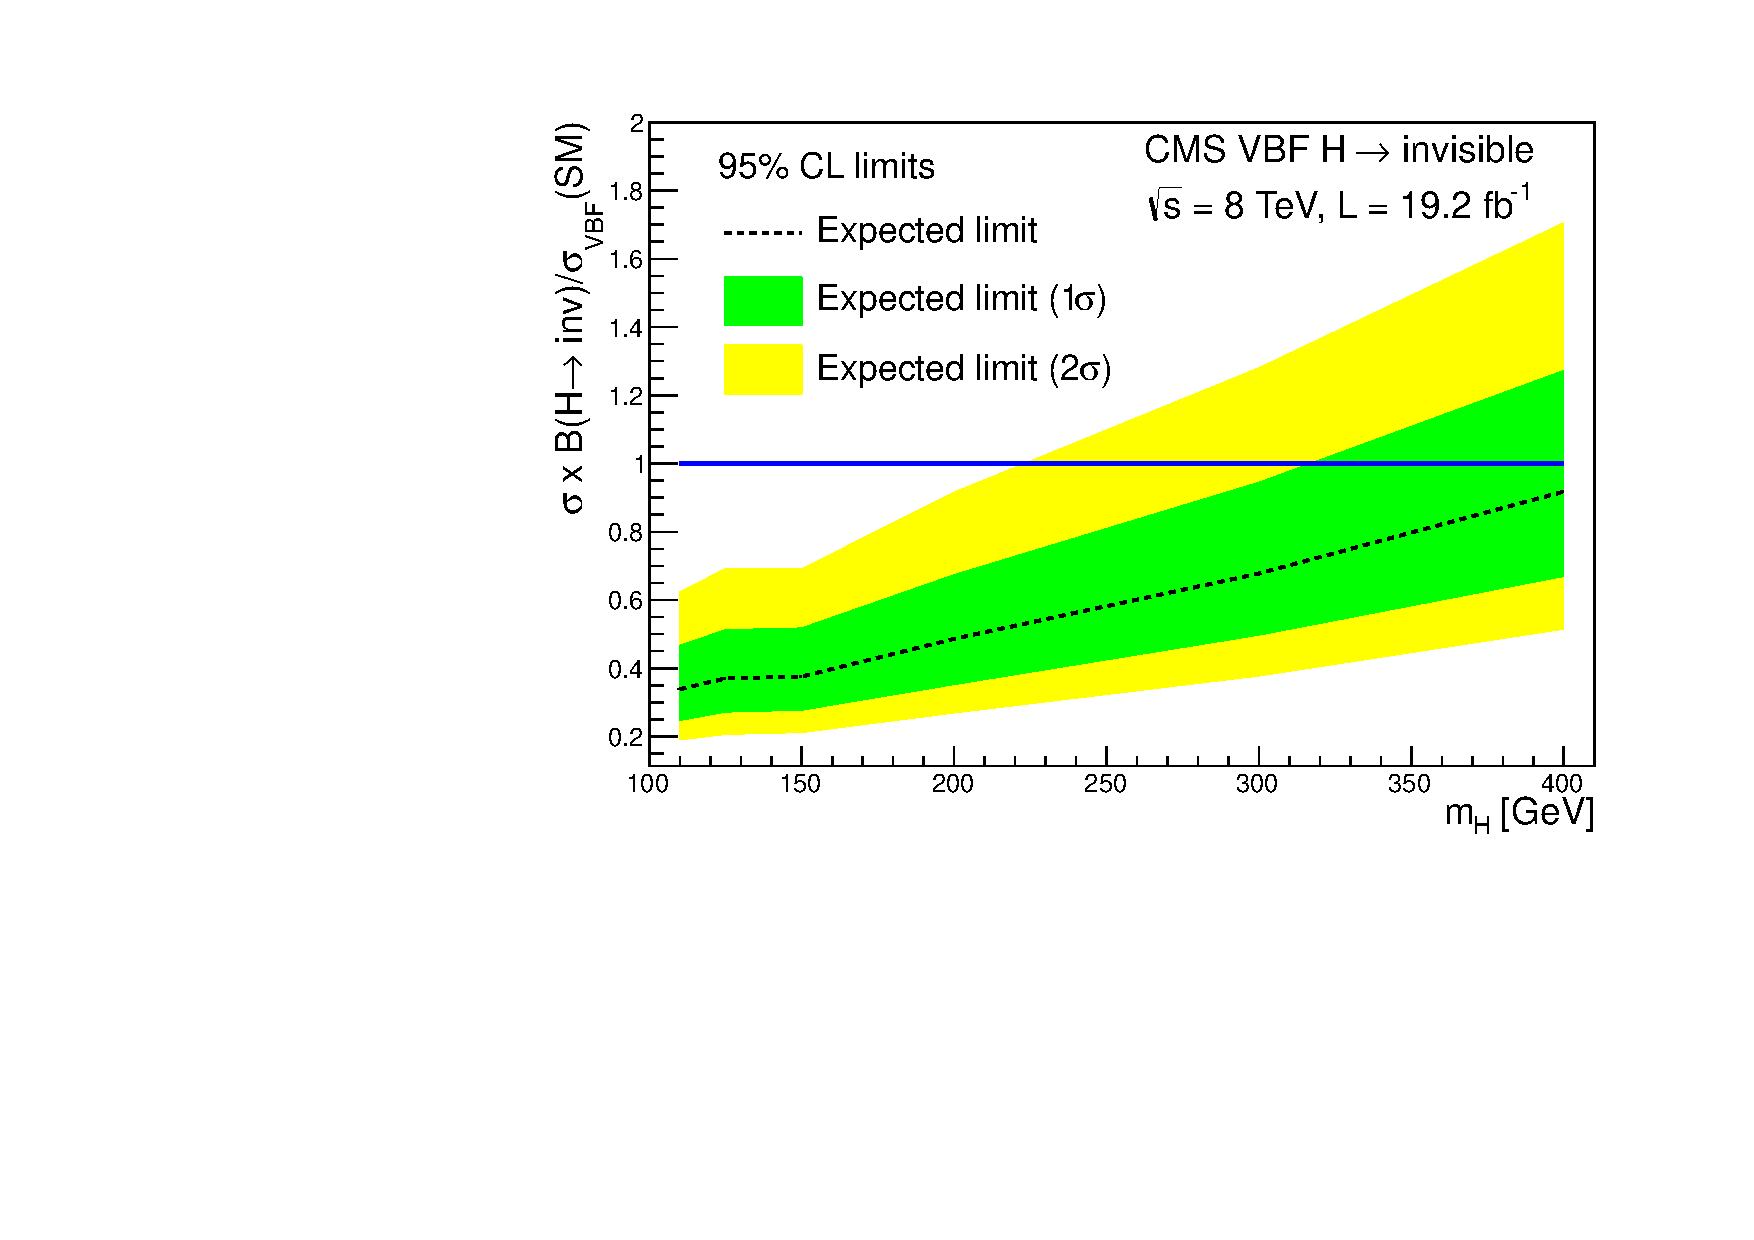
\includegraphics[clip=true,trim= 0 0 0 20,width=.52\textwidth]{TalkPics/runcbug101114/vbflimit.pdf}
        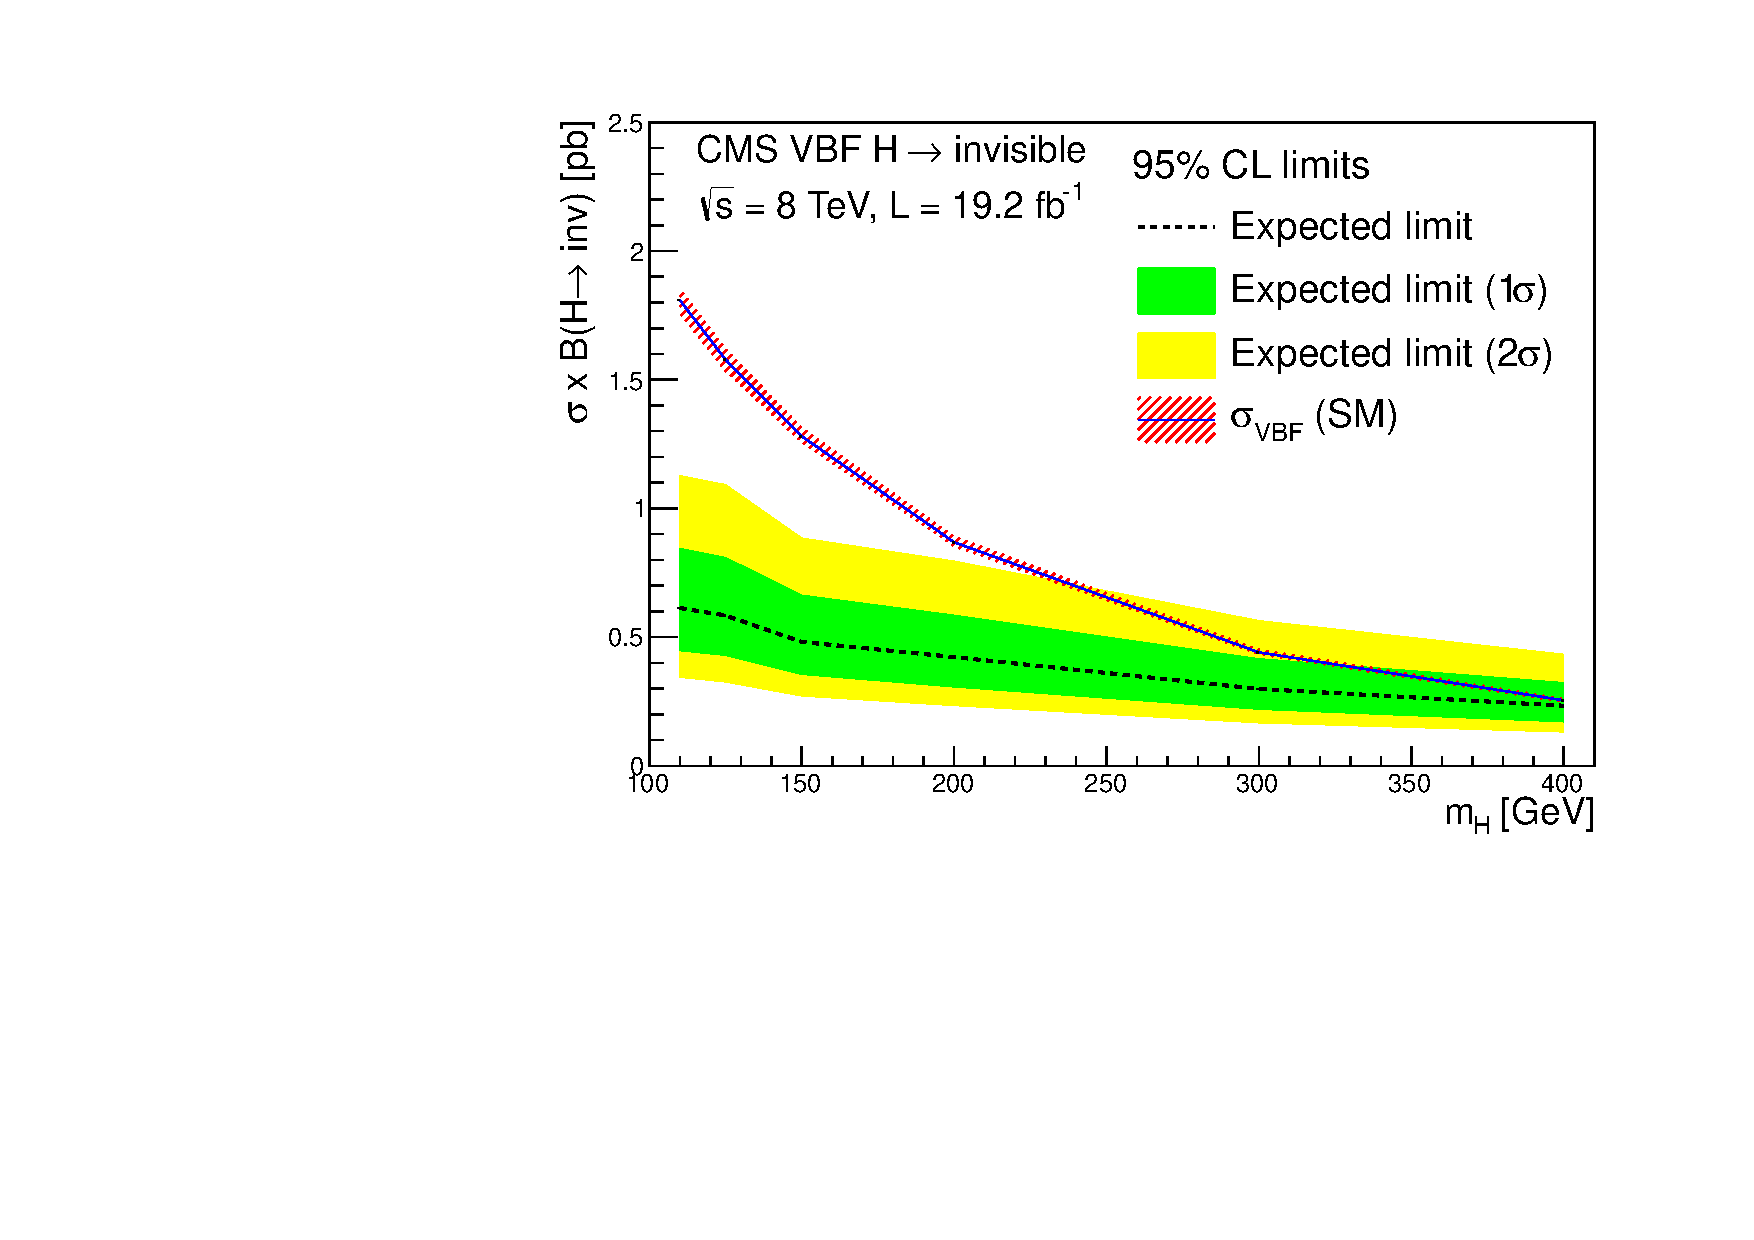
\includegraphics[clip=true,trim= 0 0 0 20,width=.52\textwidth]{TalkPics/runcbug101114/vbfxslimit.pdf}
      \end{columns}
\end{frame}

\begin{frame}
  \frametitle{Uncertainty impact table - impacts larger than 0\%}
  \vspace{-.3cm}
  \begin{block}{}
    \scriptsize
\begin{tabular}{|l|c|c|}
      \hline
Median expected limit with: & All Nuisances: 37.0\%, & No Nuisances: 14.2\% \\
\hline
\hline
Nuisance      &                Removal Effect & Addition effect \\
\hline
CMS\_eff\_m:               &      -0.5\%            &              4.8\% \\
CMS\_scale\_j:             &      -5.8\%            &              9.6\% \\
CMS\_VBFHinv\_zvv\_norm:    &      -2.6\%            &             24.7\% \\
CMS\_VBFHinv\_zvv\_stat:    &     -12.7\%            &             67.0\% \\
CMS\_VBFHinv\_wmu\_norm:    &      -1.1\%            &              6.2\% \\
CMS\_VBFHinv\_wmu\_stat:    &      -0.5\%            &              3.4\% \\
CMS\_VBFHinv\_wel\_norm:    &      -0.5\%            &              2.7\% \\
CMS\_VBFHinv\_wel\_stat:    &      -0.5\%            &              4.1\% \\
CMS\_VBFHinv\_tau\_eff:     &      -0.5\%            &              5.5\% \\
CMS\_VBFHinv\_tau\_extrapfacunc: & -4.2\%            &             24.7\% \\
CMS\_VBFHinv\_wtau\_norm:        & -1.6\%            &             11.7\% \\
CMS\_VBFHinv\_wtau\_stat:        & -2.1\%            &             13.7\% \\
CMS\_VBFHinv\_zvv\_extrapfacunc: & -8.7\%            &             53.3\% \\
CMS\_VBFHinv\_qcd\_norm:         & -1.1\%            &              4.8\% \\
      \hline
    \end{tabular}    
  \end{block}
\end{frame}

%!!SUMMARY
\begin{frame}
  \frametitle{Summary}
  \label{lastframe}
  \begin{block}{}
    \scriptsize
    \begin{itemize}
    \item Bug found and fixed
    \item New expected limit is 37\%
    \item AN updated apart from QCD
    \item Still need to answer Paolo's questions about the source of the gain
    \item[-] Will run light trees with prompt data and apply new selection
    \item[-] Should take 1-2 days
    \end{itemize}
  \end{block}
\end{frame}

\begin{frame}
  \frametitle{Backup}
\end{frame}

\begin{frame}
  \frametitle{New control plots - mumu}
  \begin{columns}
    \column{.5\textwidth}
    \begin{block}{Jet 1 pt}
      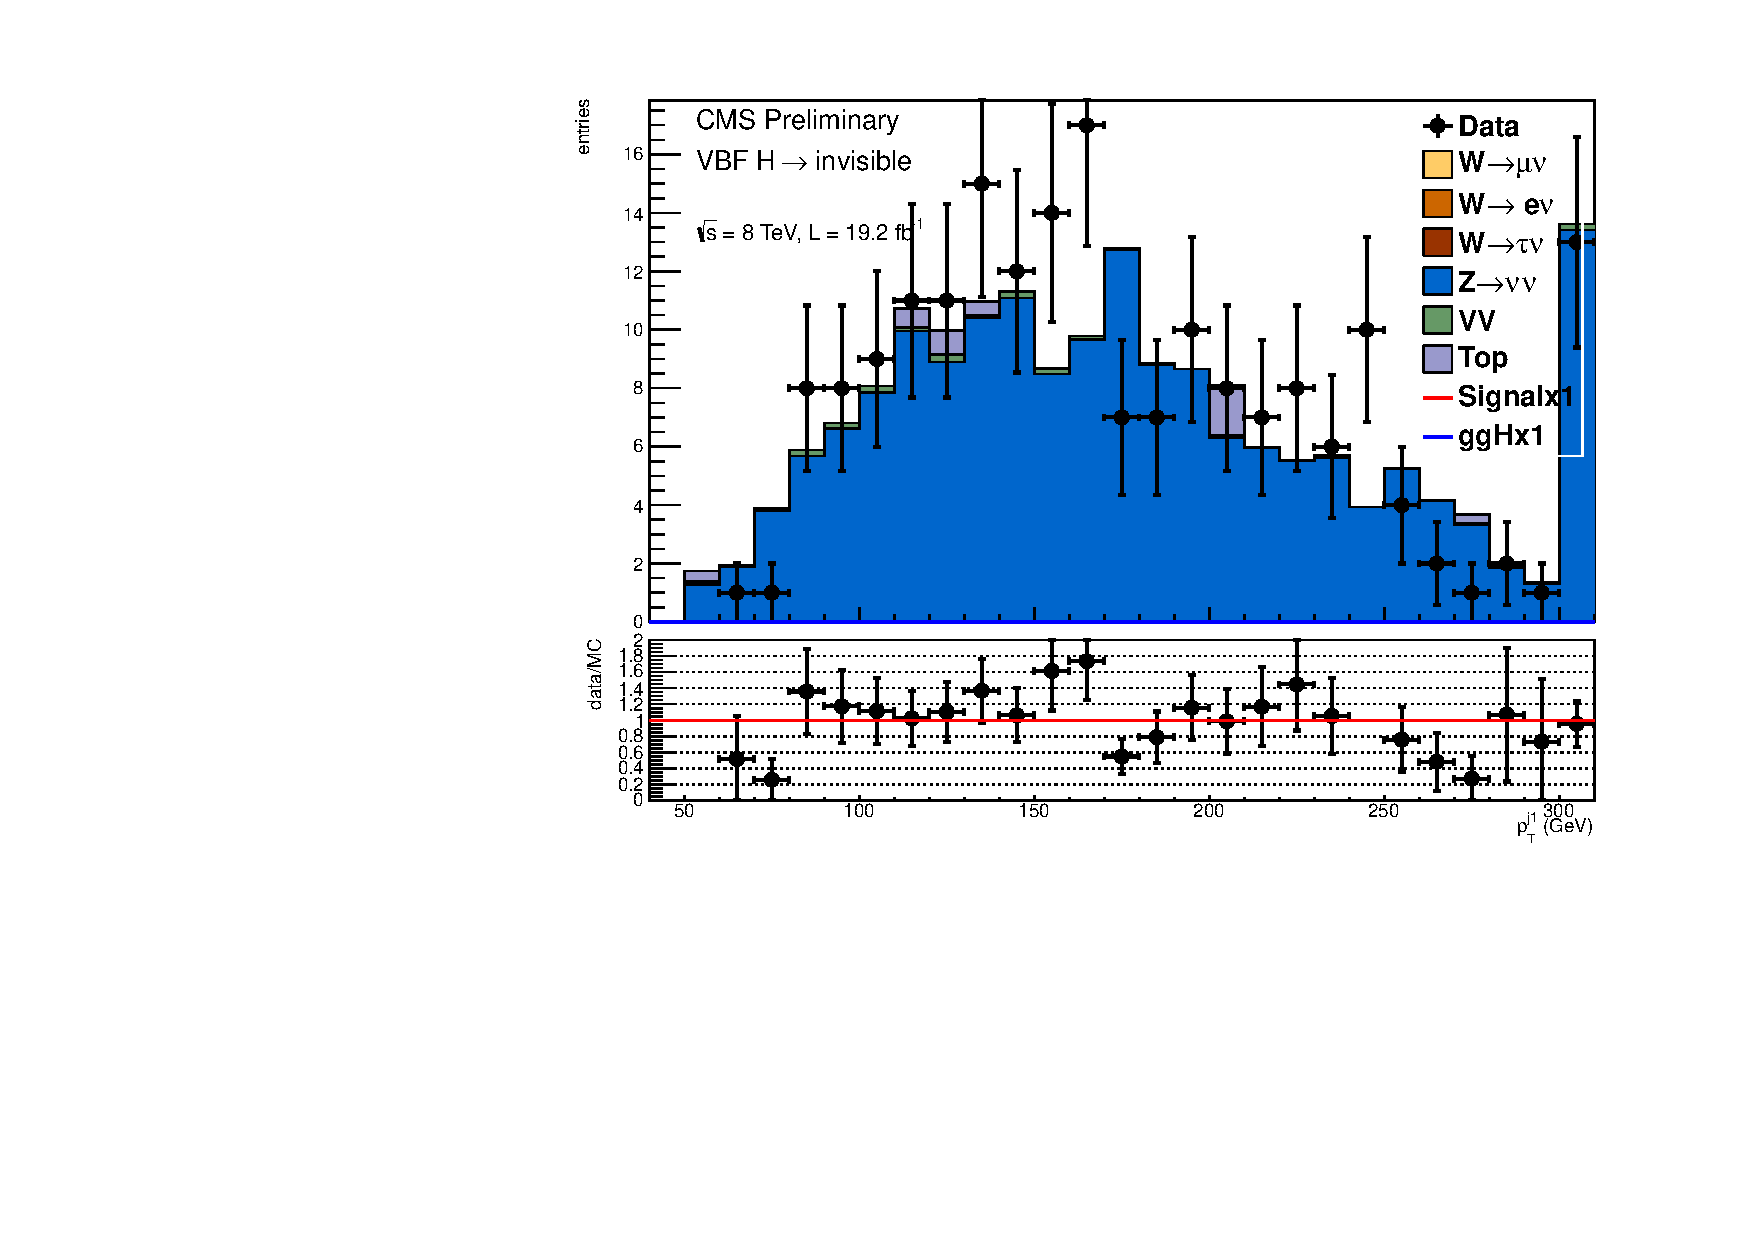
\includegraphics[width=\textwidth]{TalkPics/runcbug101114/output_presel/mumu_jet1_pt.pdf}
    \end{block}
    \column{.5\textwidth}
    \begin{block}{Jet 2 pt}
      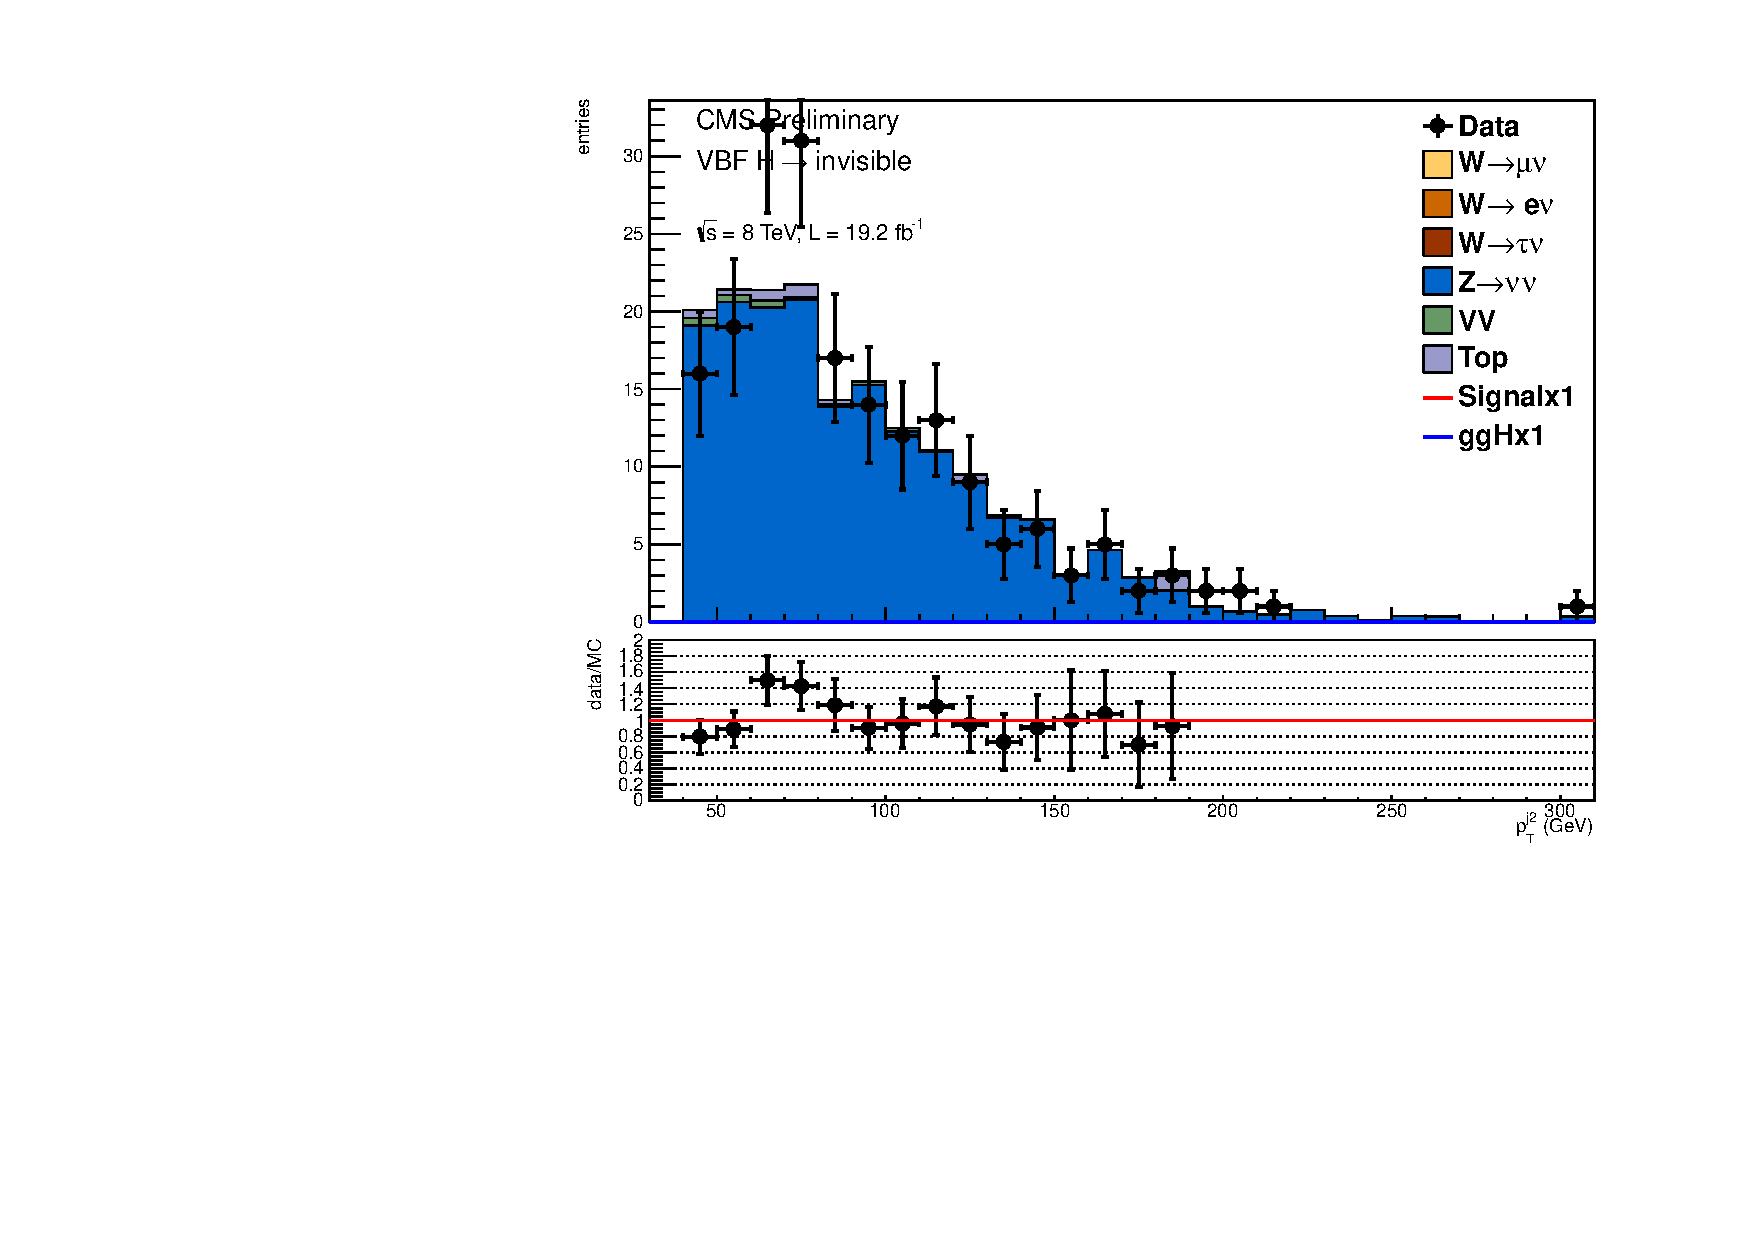
\includegraphics[width=\textwidth]{TalkPics/runcbug101114/output_presel/mumu_jet2_pt.pdf}
    \end{block}

  \end{columns}
\end{frame}

\begin{frame}
  \frametitle{New control plots - mumu}
  \begin{columns}
    \column{.5\textwidth}
    \begin{block}{METnomu}
      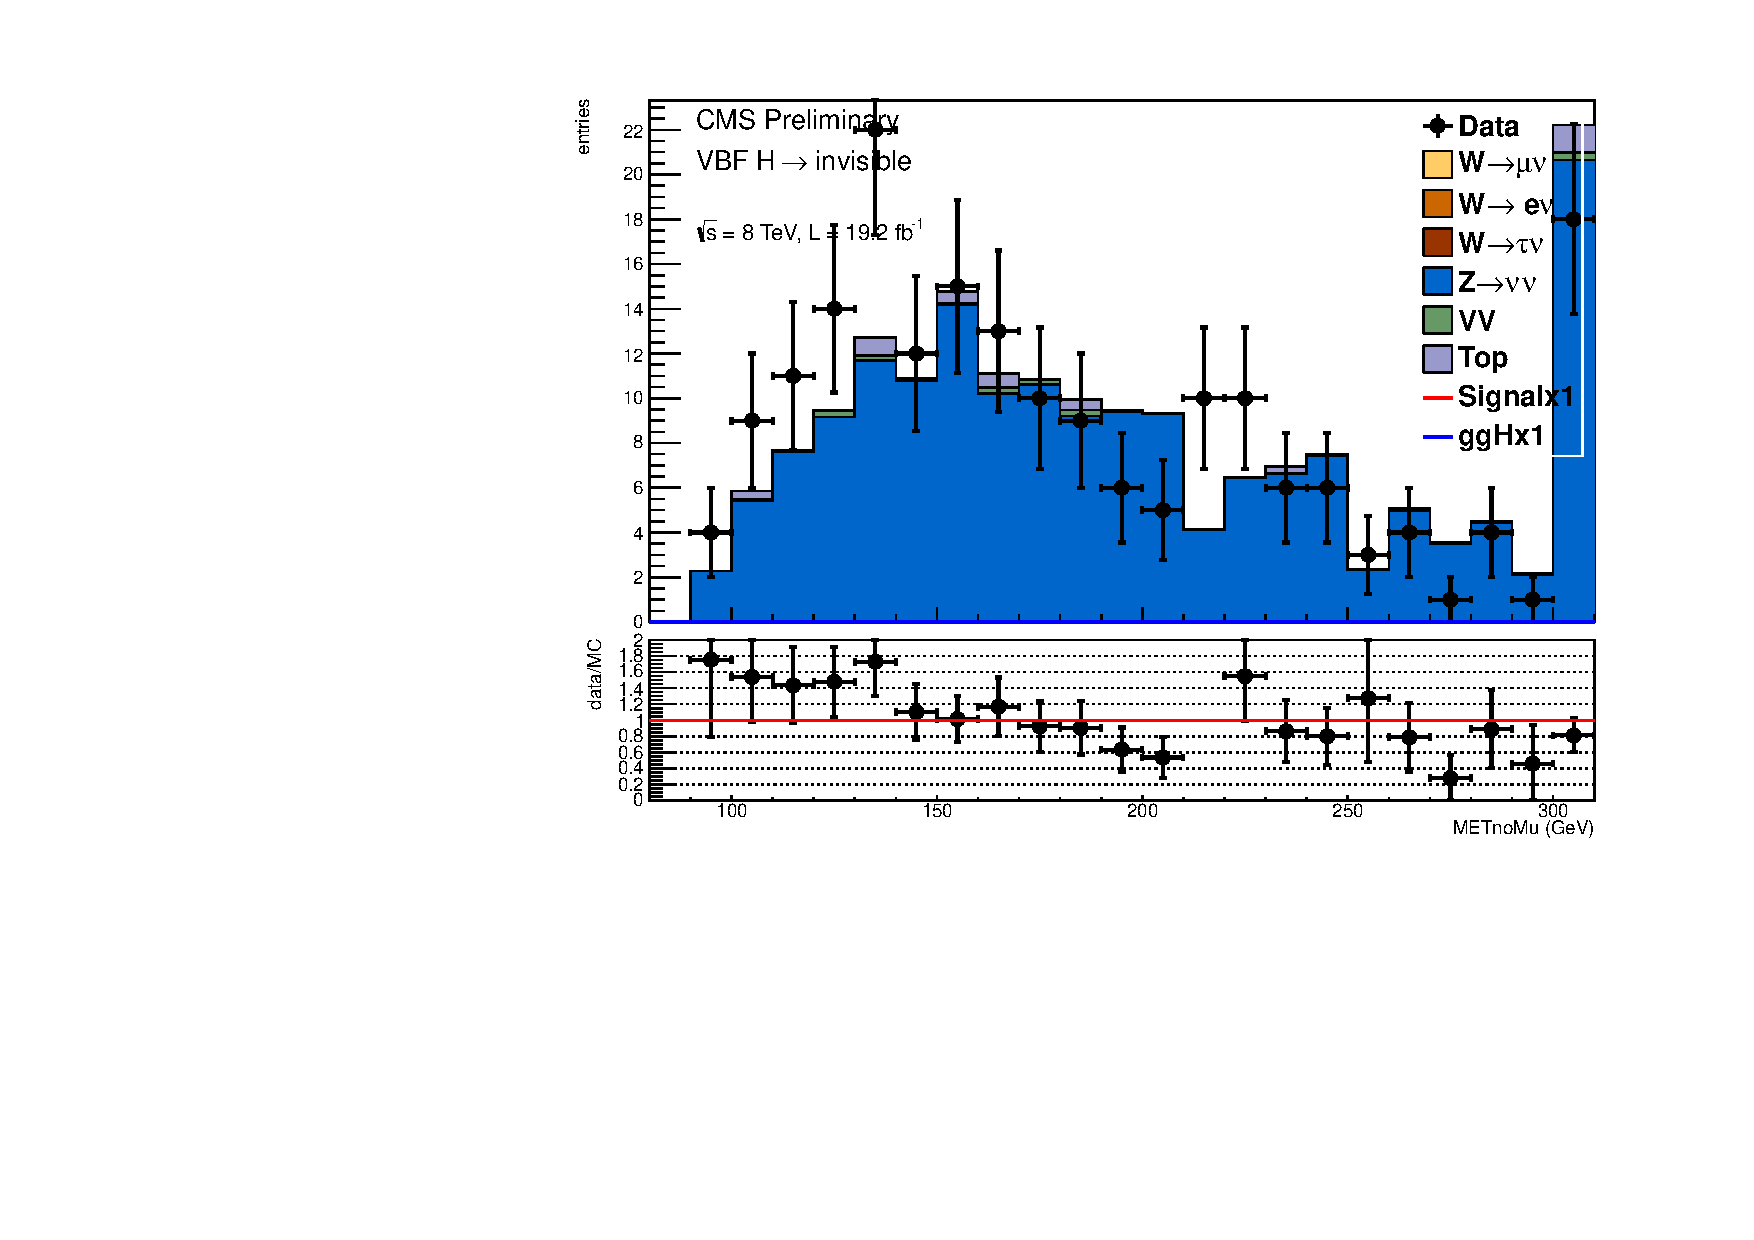
\includegraphics[width=\textwidth]{TalkPics/runcbug101114/output_presel/mumu_metnomuons.pdf}
    \end{block}
    \column{.5\textwidth}
    \begin{block}{METnomusig}
      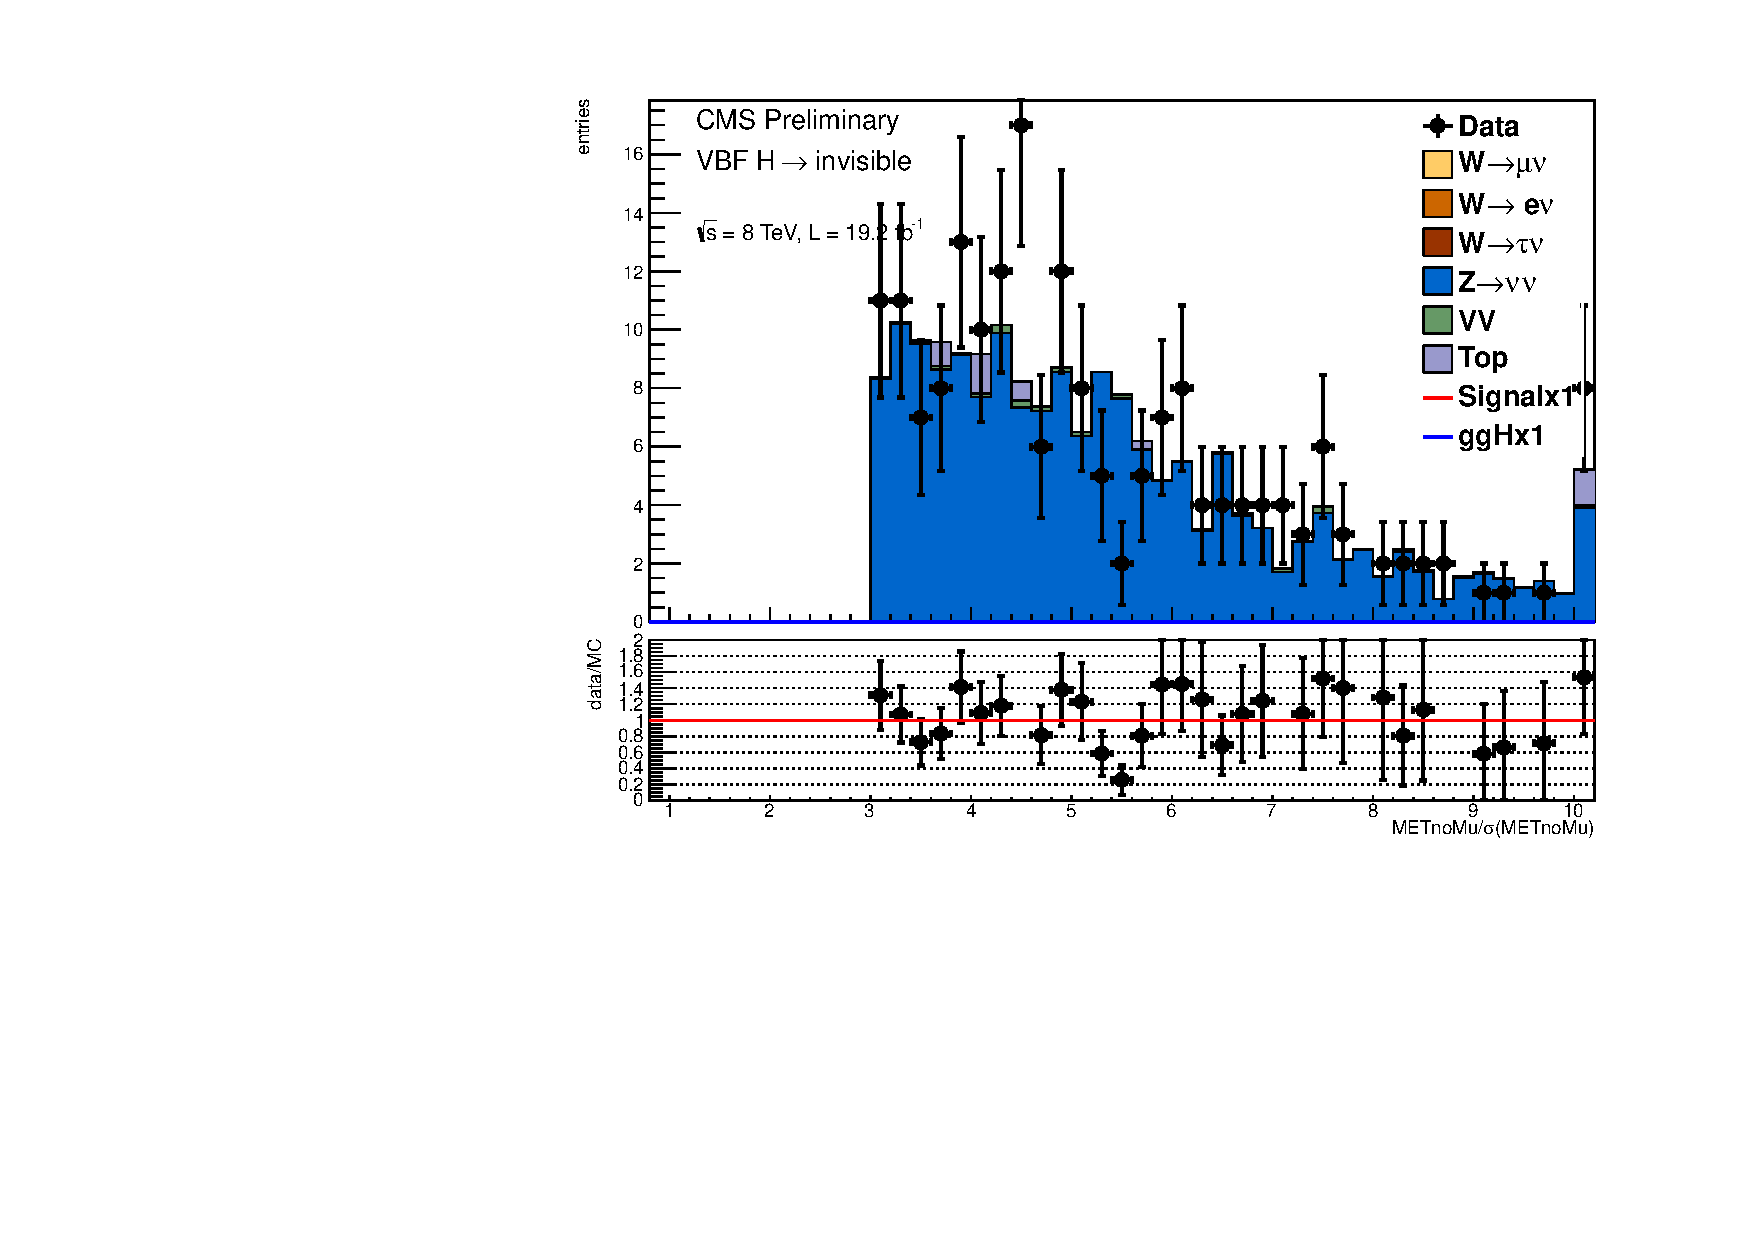
\includegraphics[width=\textwidth]{TalkPics/runcbug101114/output_presel/mumu_metnomu_significance.pdf}
    \end{block}

  \end{columns}
\end{frame}

\begin{frame}
  \frametitle{New control plots - mumu }
  \begin{columns}
    \column{.5\textwidth}
    \begin{block}{Mjj}
      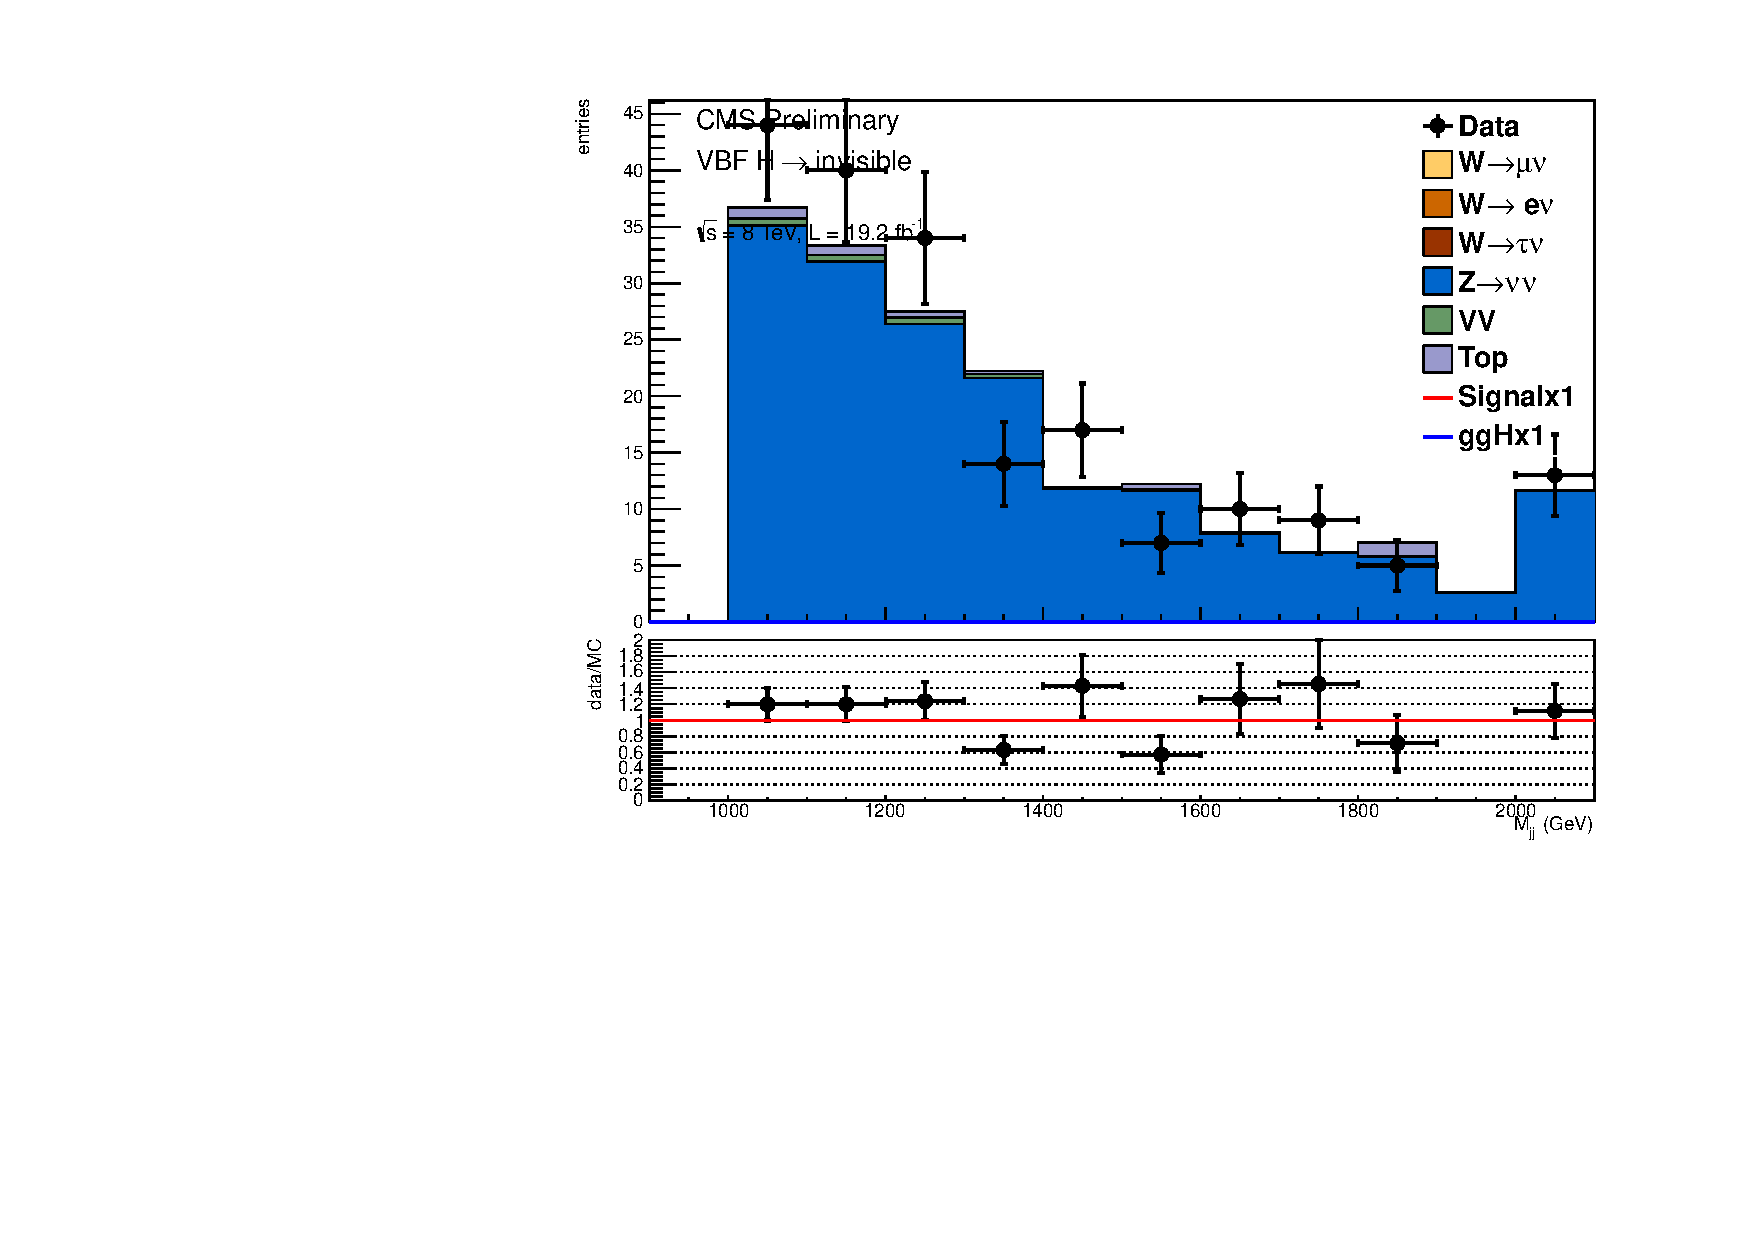
\includegraphics[width=\textwidth]{TalkPics/runcbug101114/output_presel/mumu_dijet_M.pdf}
    \end{block}
    \column{.5\textwidth}
    \begin{block}{dijet-metnomu pt fraction}
      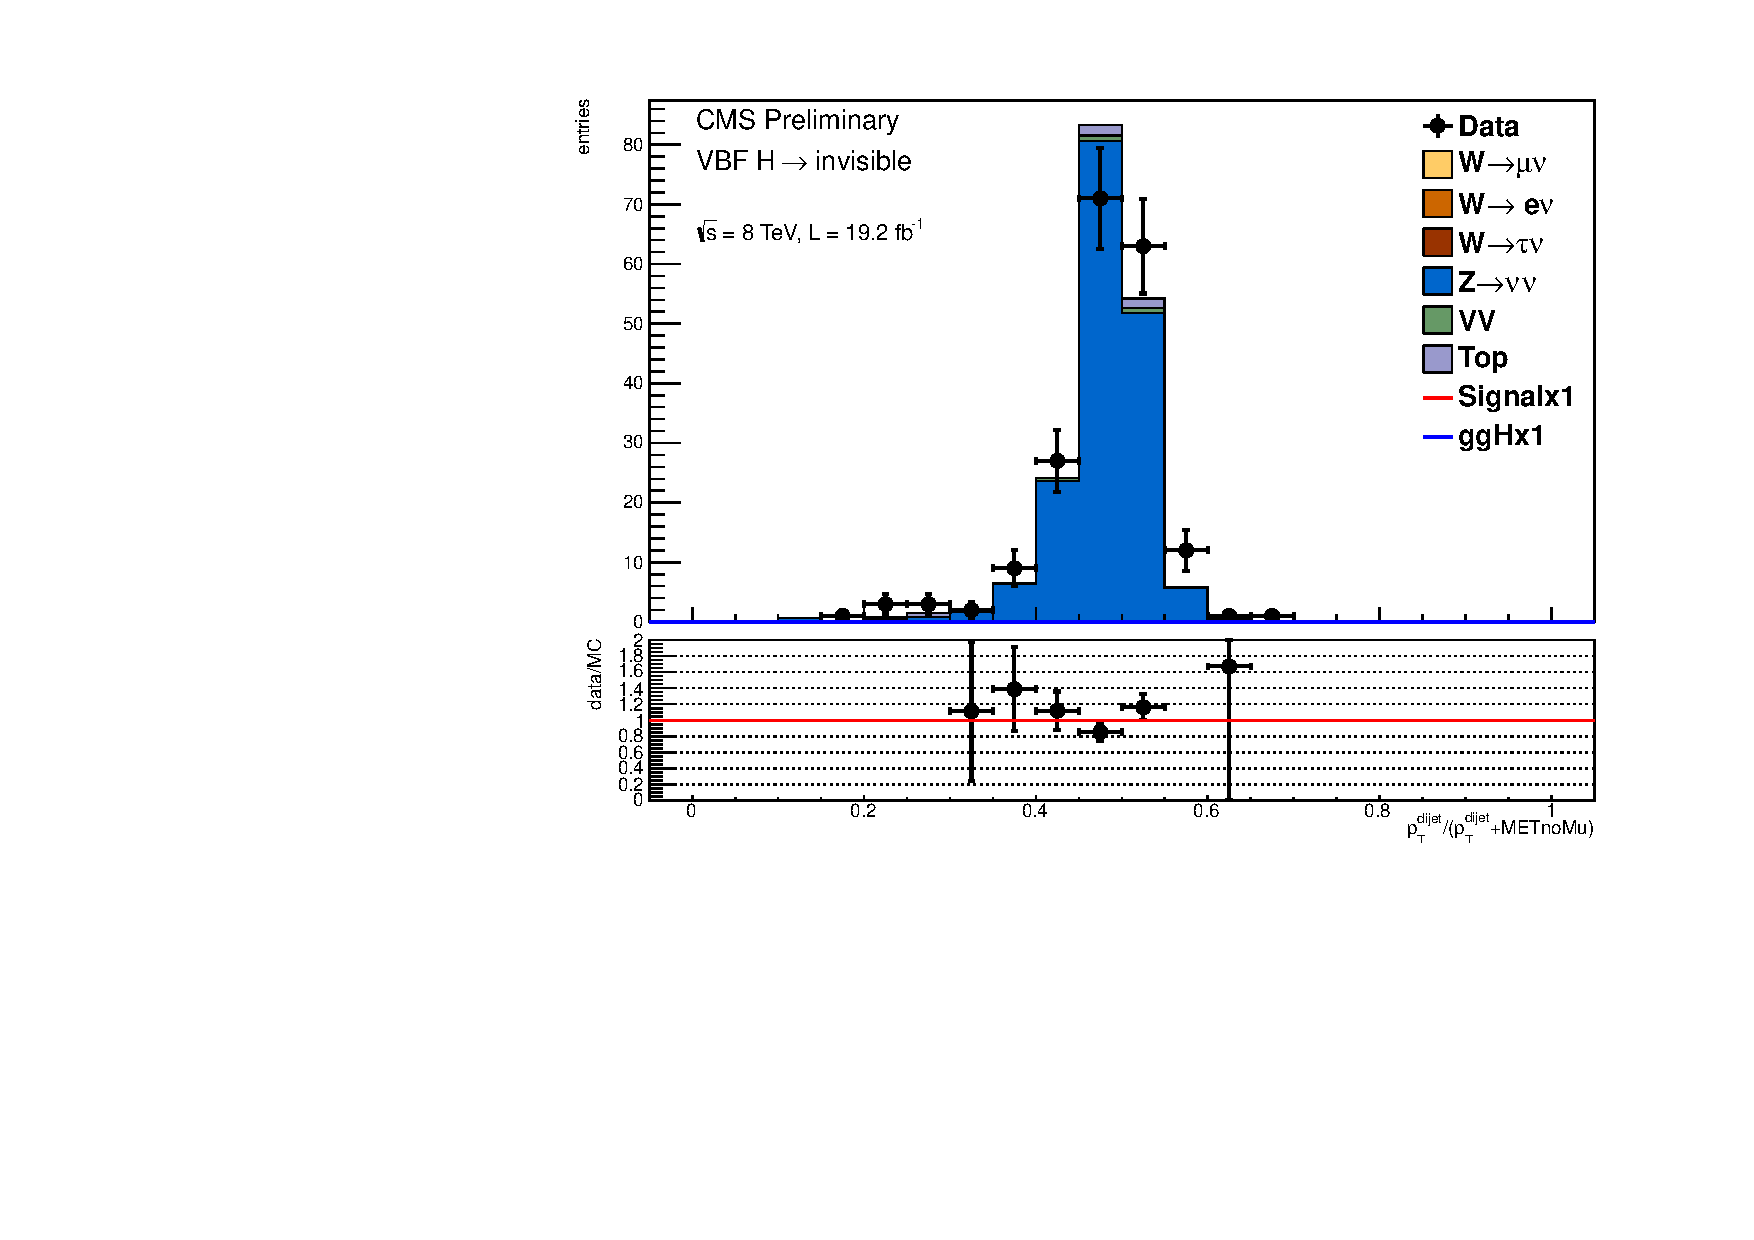
\includegraphics[width=\textwidth]{TalkPics/runcbug101114/output_presel/mumu_dijetmetnomu_ptfraction.pdf}
    \end{block}
  \end{columns}
\end{frame}

\begin{frame}
  \frametitle{New control plots -mumu}
  \begin{columns}
    \column{.5\textwidth}
    \begin{block}{Dphijj}
      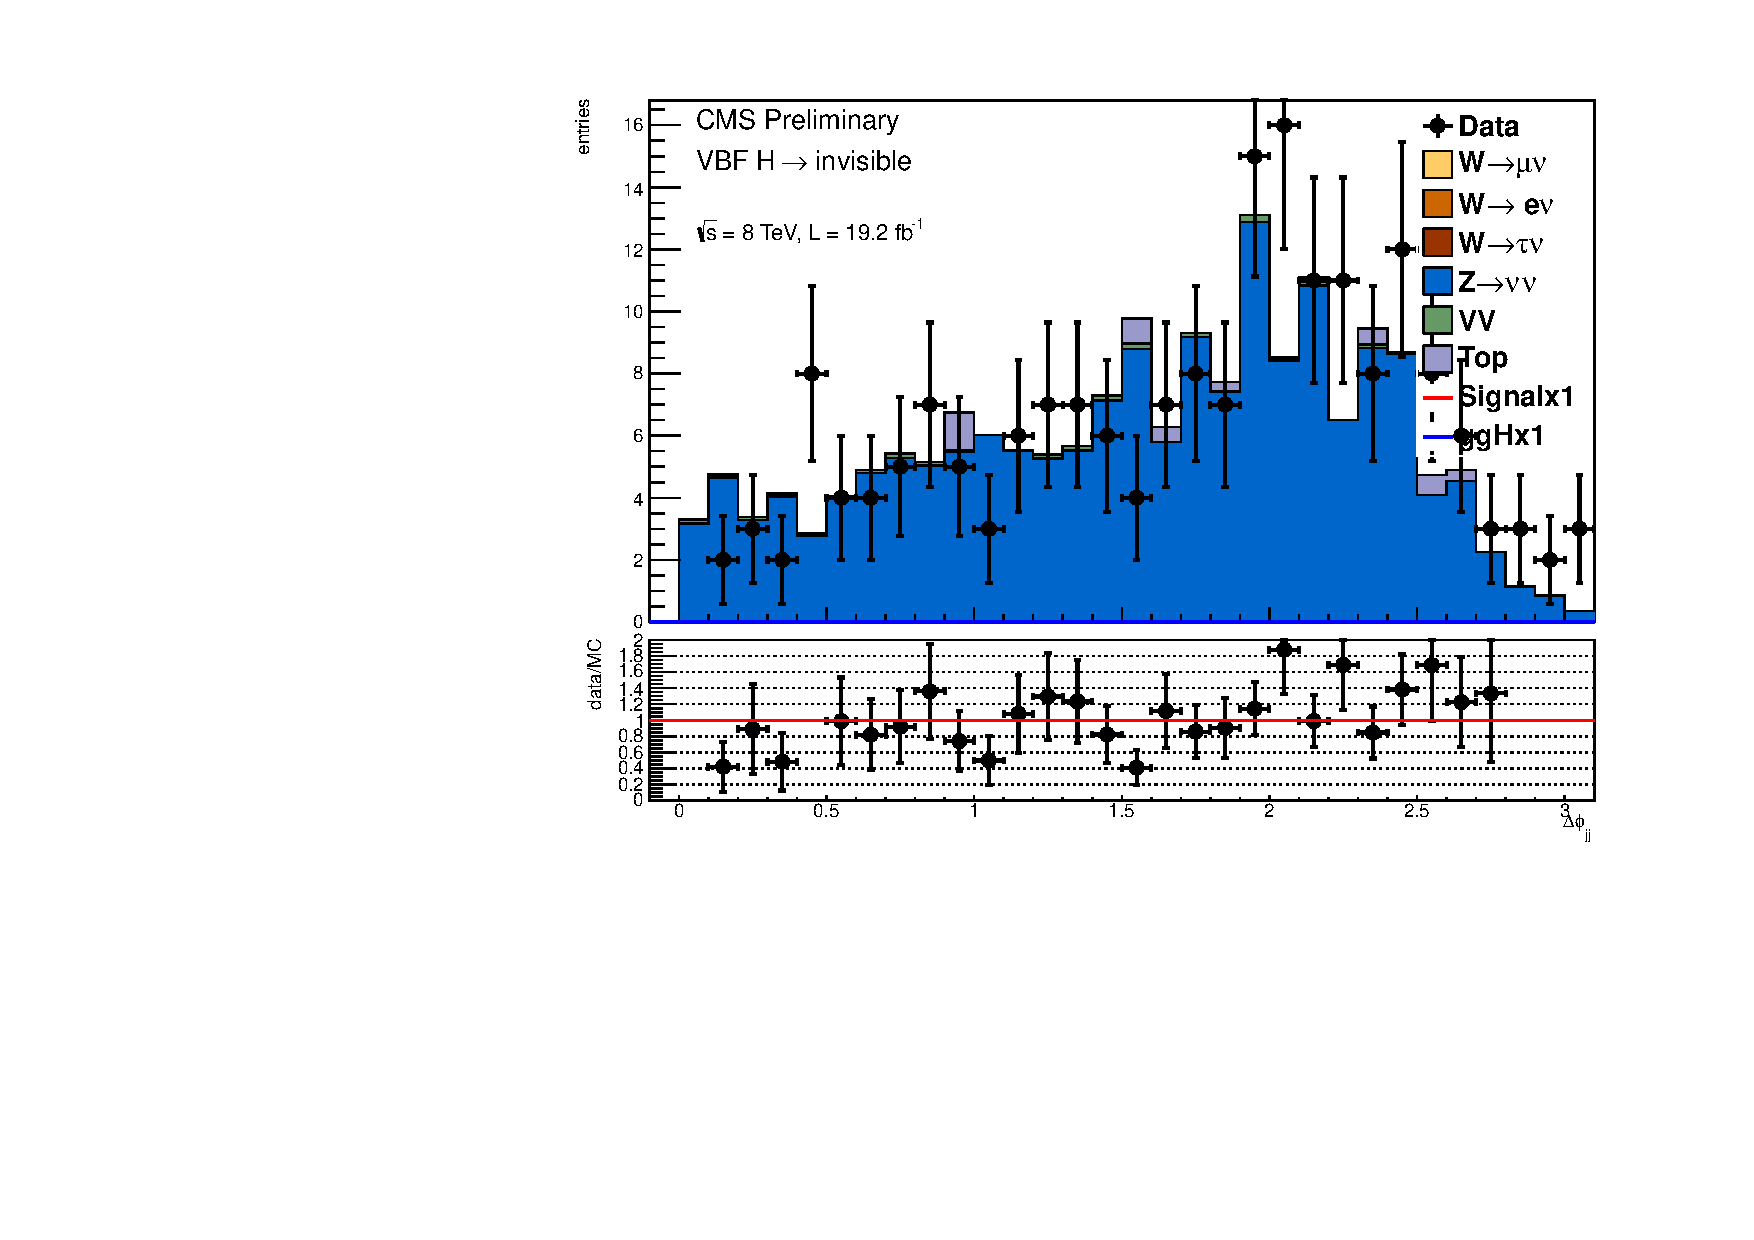
\includegraphics[width=\textwidth]{TalkPics/runcbug101114/output_presel/mumu_dijet_dphi.pdf}
    \end{block}
    \column{.5\textwidth}
    \begin{block}{Detajj}
      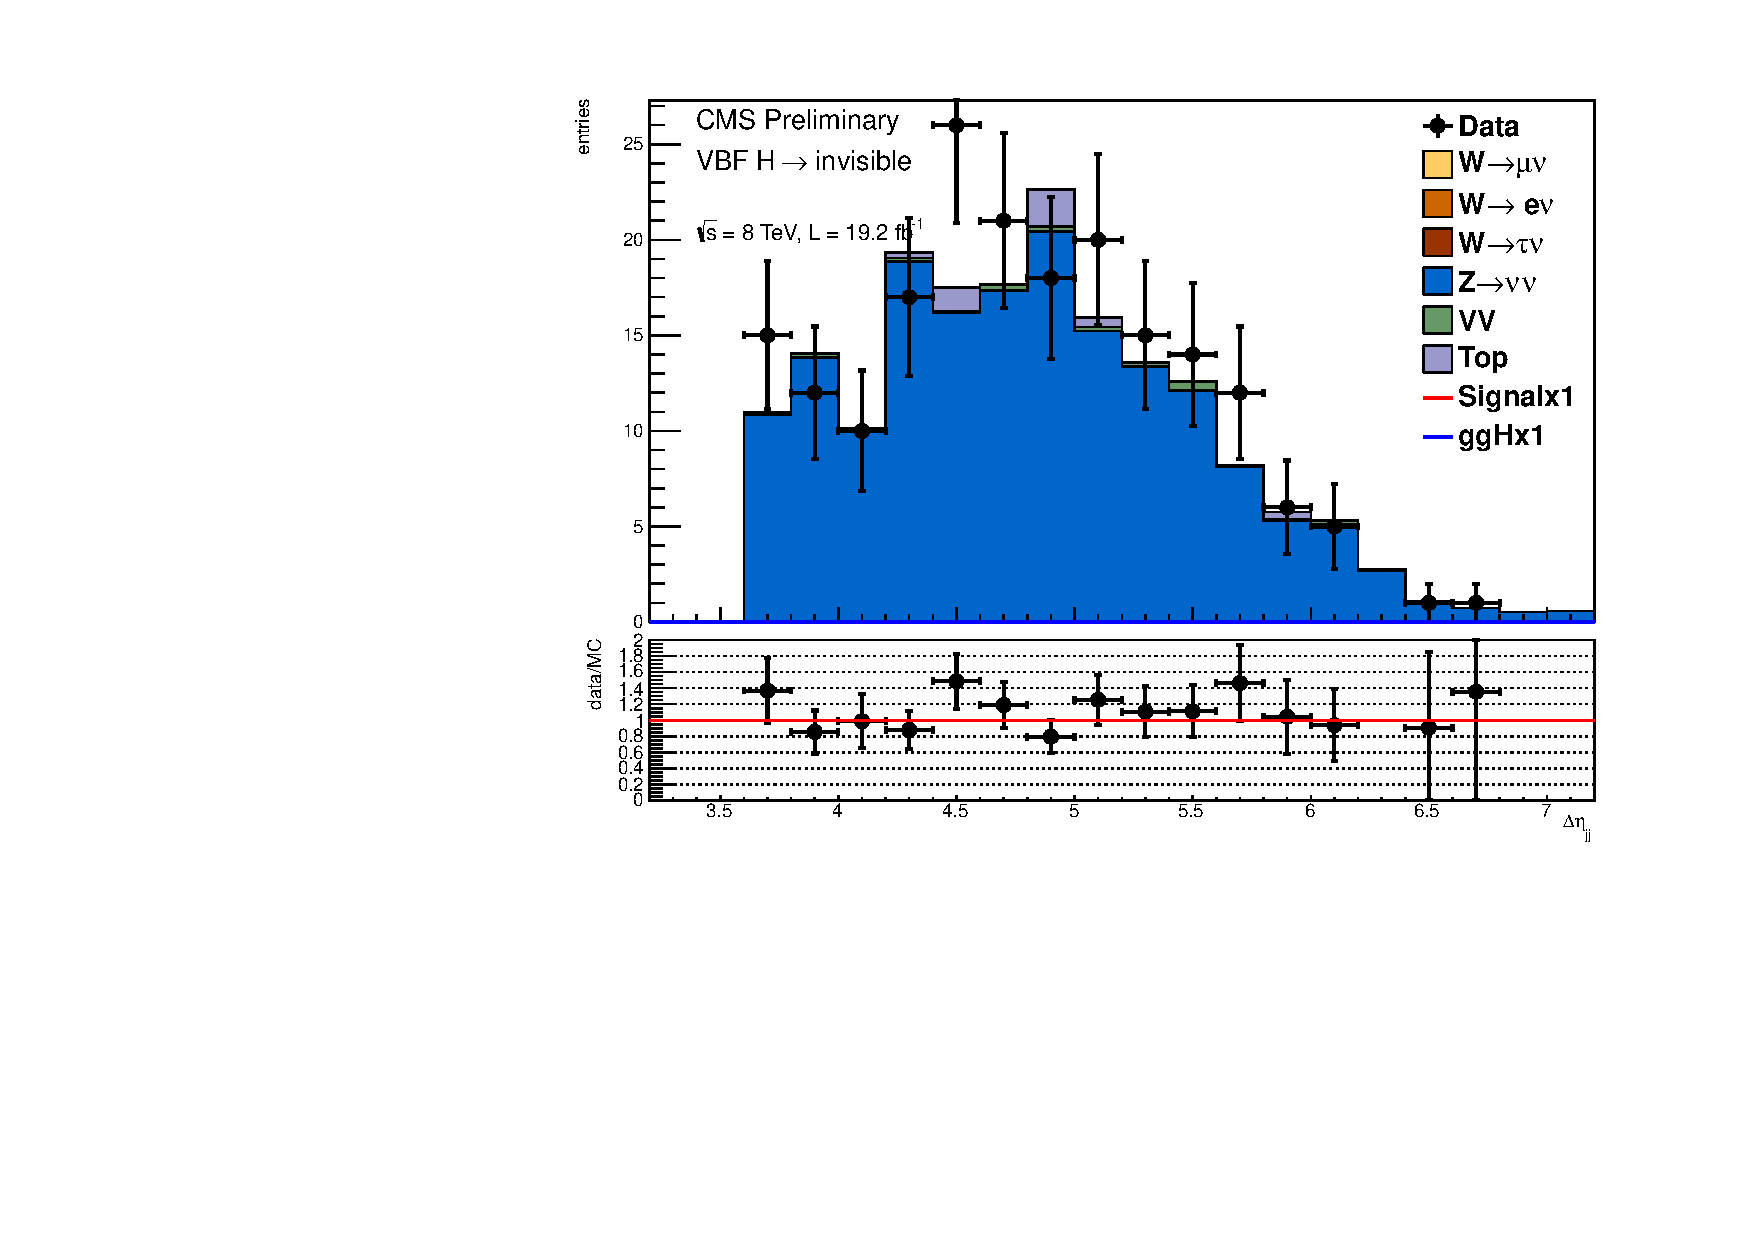
\includegraphics[width=\textwidth]{TalkPics/runcbug101114/output_presel/mumu_dijet_deta.pdf}
    \end{block}

  \end{columns}
\end{frame}

\begin{frame}
  \frametitle{New control plots -mumu}
  \begin{columns}
    \column{.5\textwidth}
    \begin{block}{Leading jets-met mindphi}
      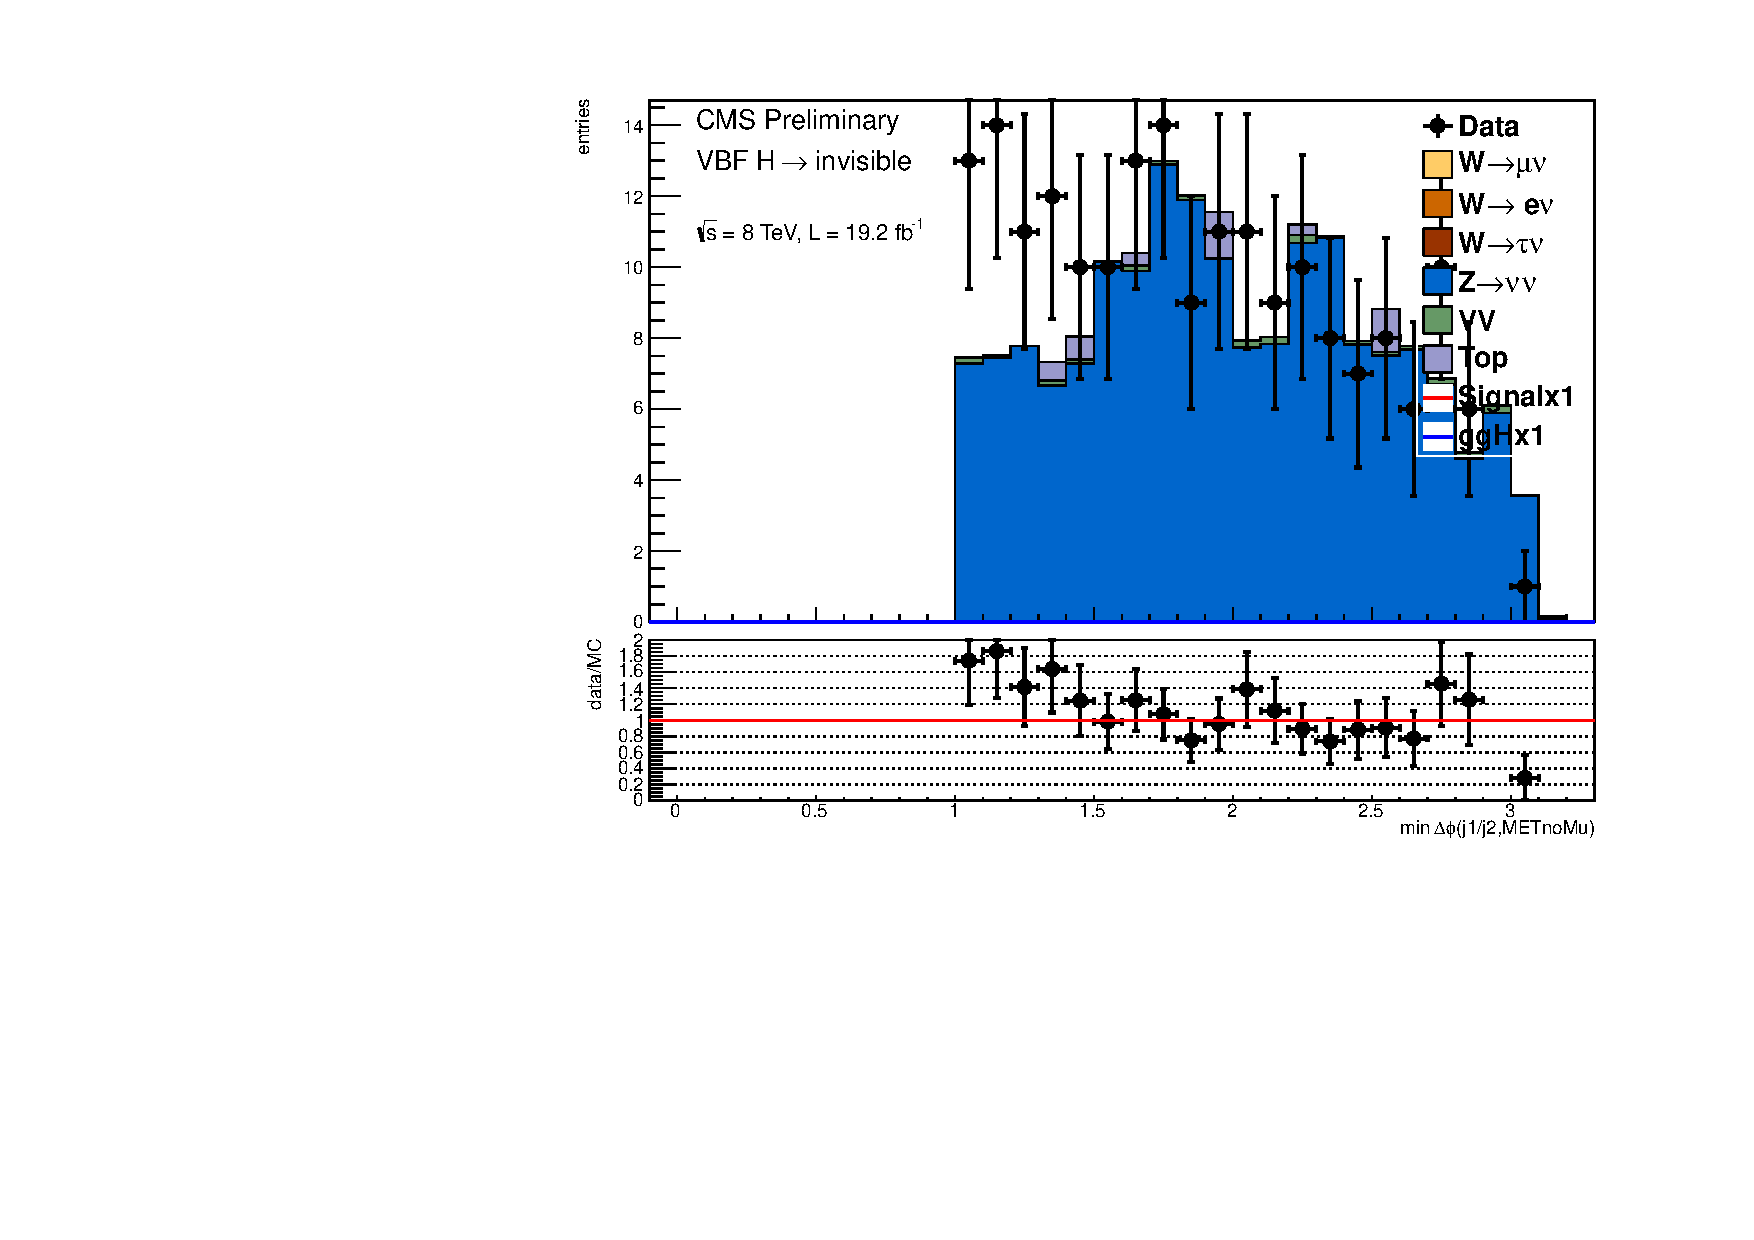
\includegraphics[width=\textwidth]{TalkPics/runcbug101114/output_presel/mumu_jetmetnomu_mindphi.pdf}
    \end{block}
    \column{.5\textwidth}
    \begin{block}{All jet-met mindphi}
      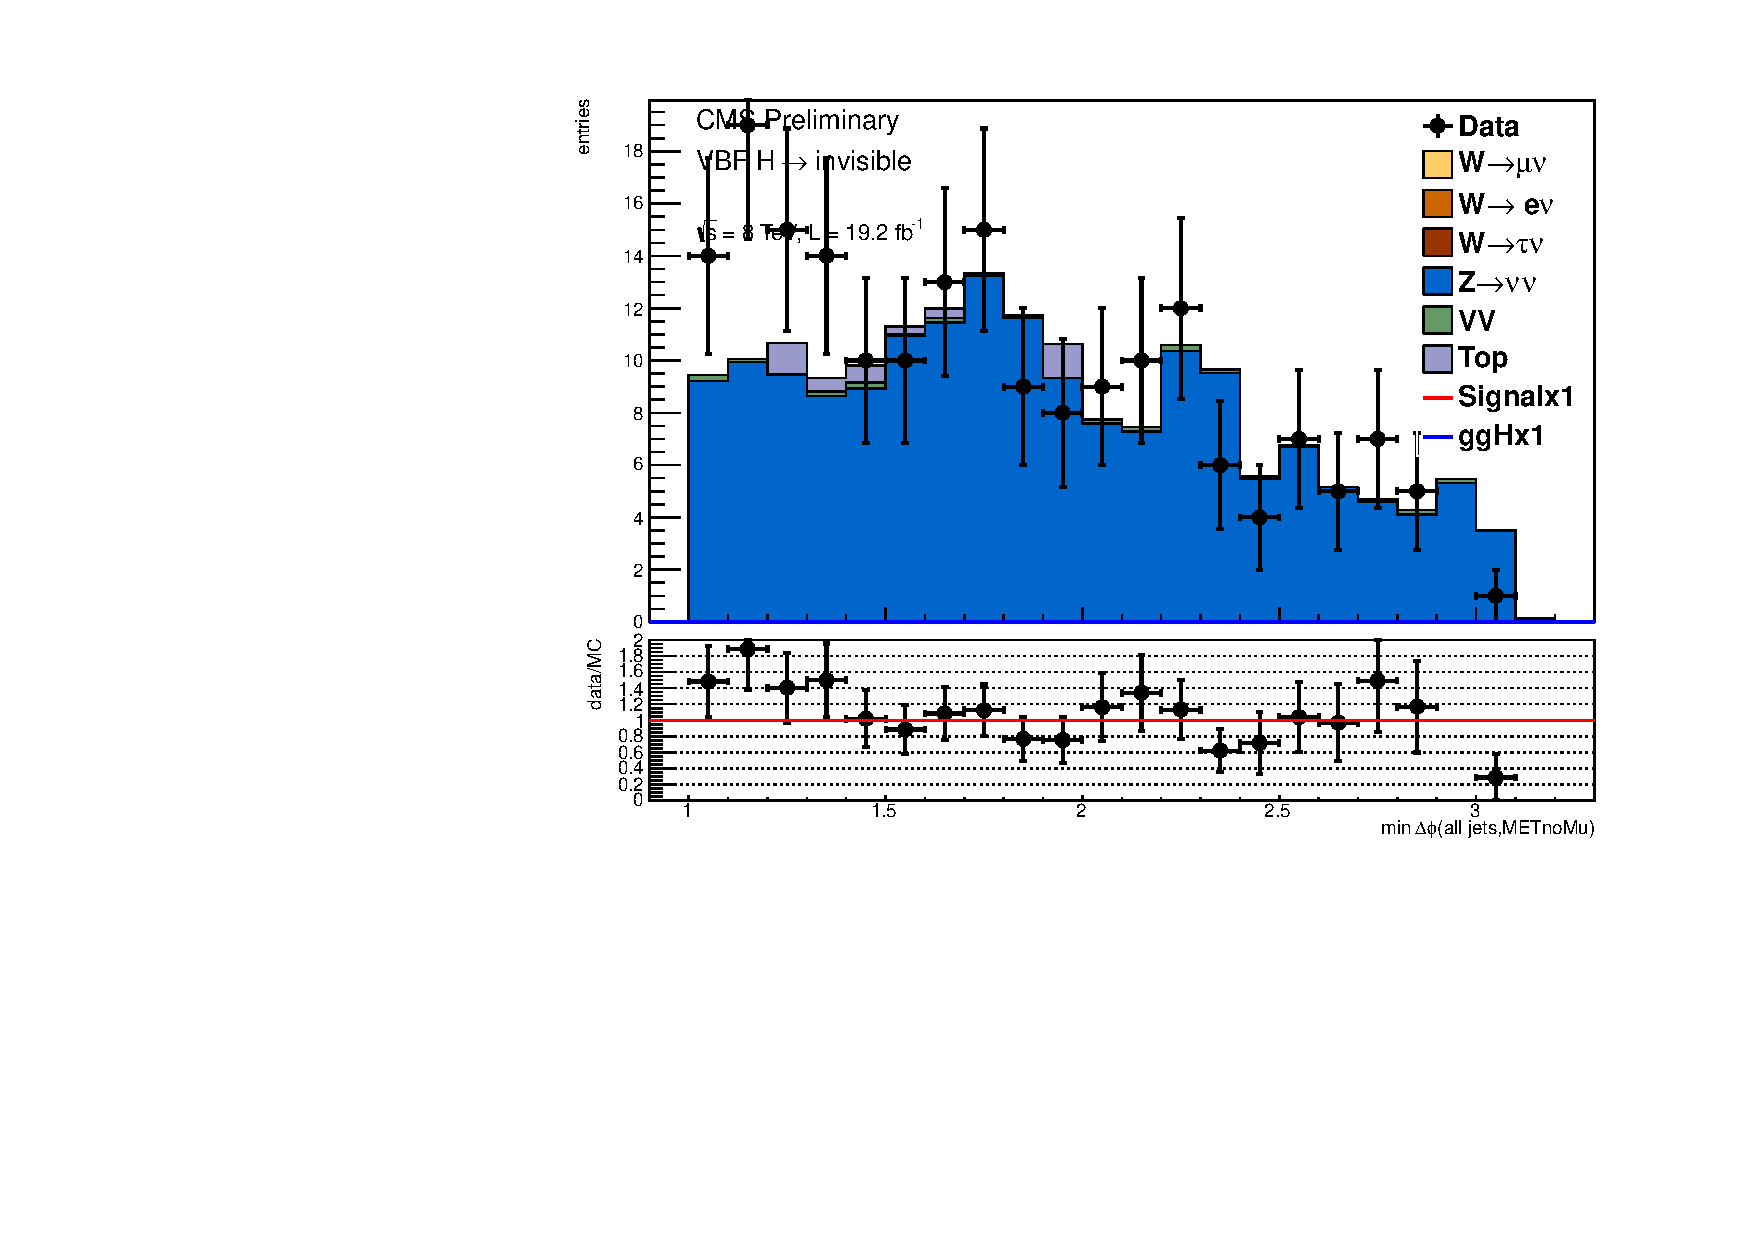
\includegraphics[width=\textwidth]{TalkPics/runcbug101114/output_presel/mumu_alljetsmetnomu_mindphi.pdf}
    \end{block}

  \end{columns}
\end{frame}

\begin{frame}
  \frametitle{New control plots - top}
  \begin{columns}
    \column{.5\textwidth}
    \begin{block}{Jet 1 pt}
      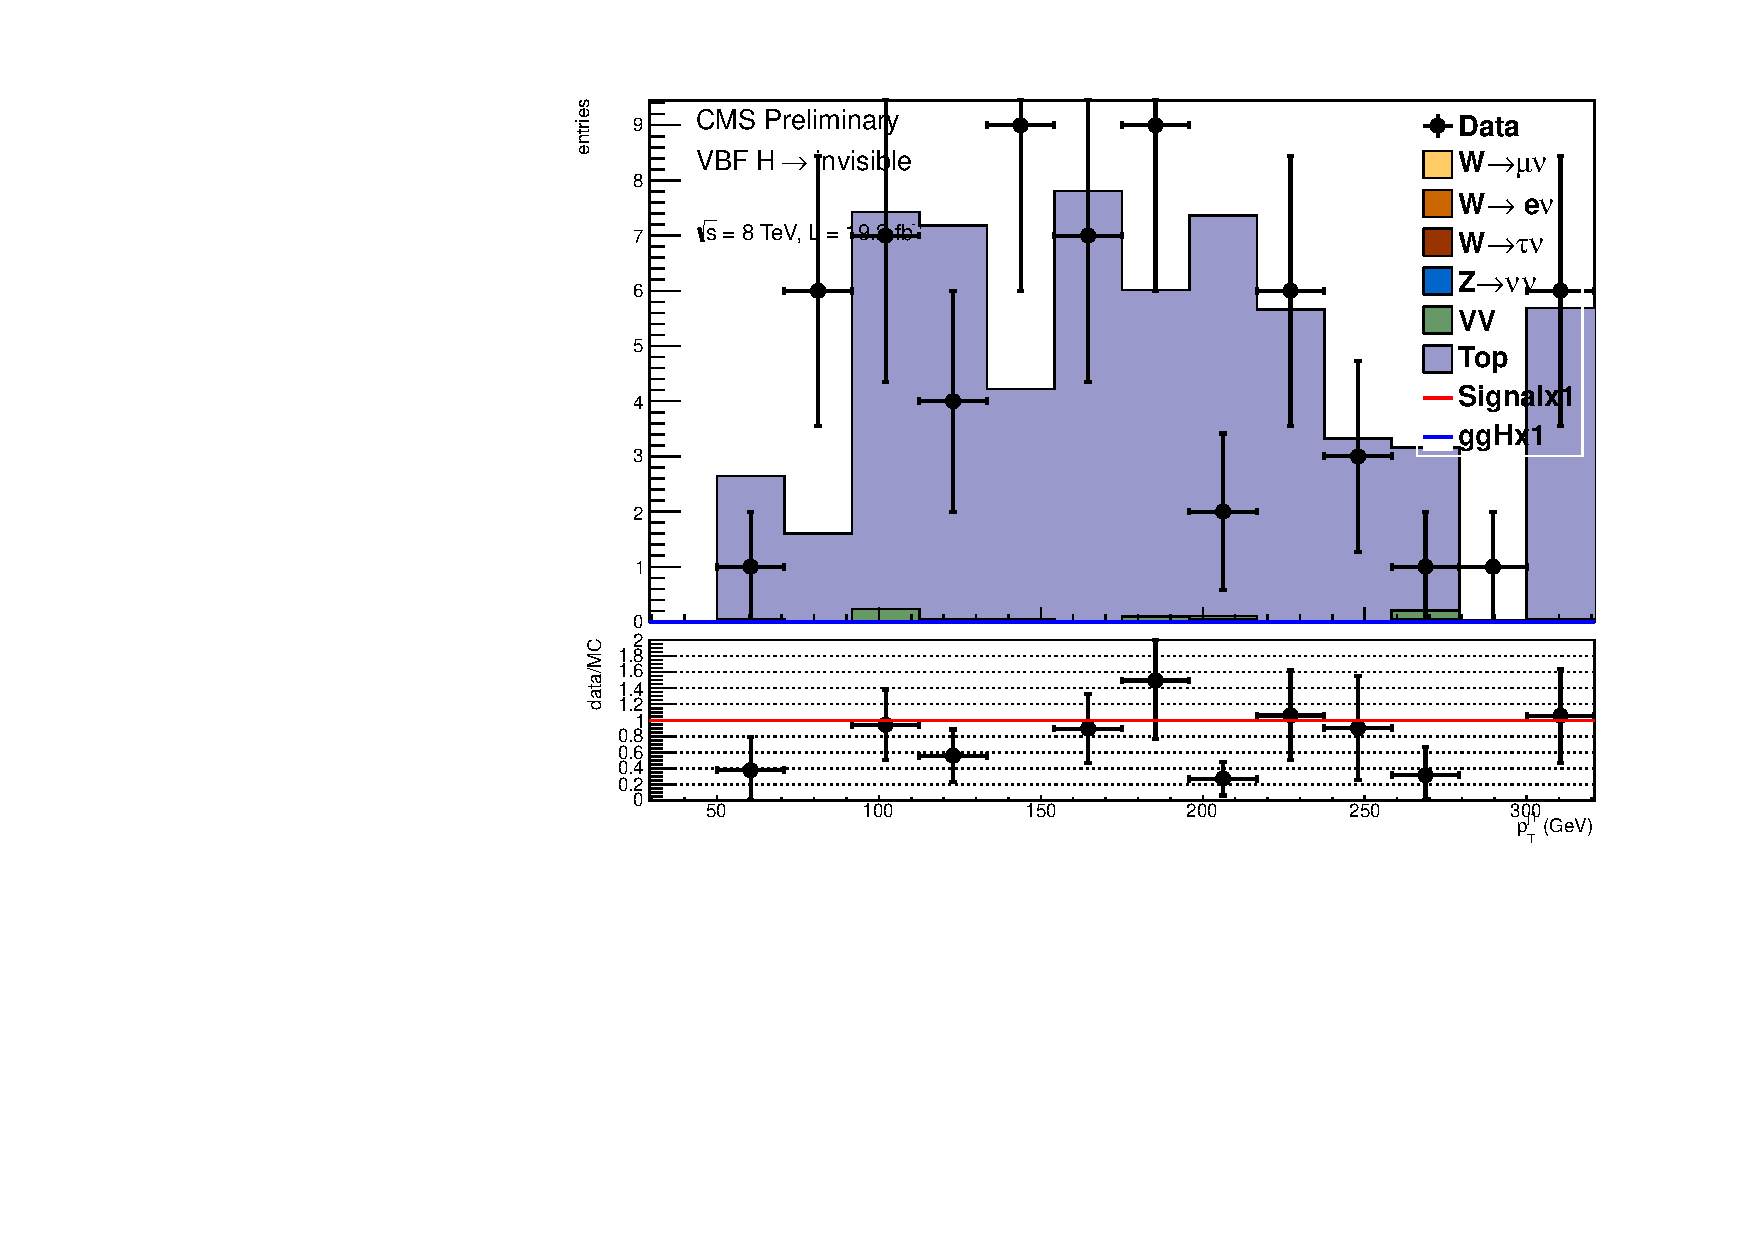
\includegraphics[width=\textwidth]{TalkPics/runcbug101114/output_presel/top_jet1_pt.pdf}
    \end{block}
    \column{.5\textwidth}
    \begin{block}{Jet 2 pt}
      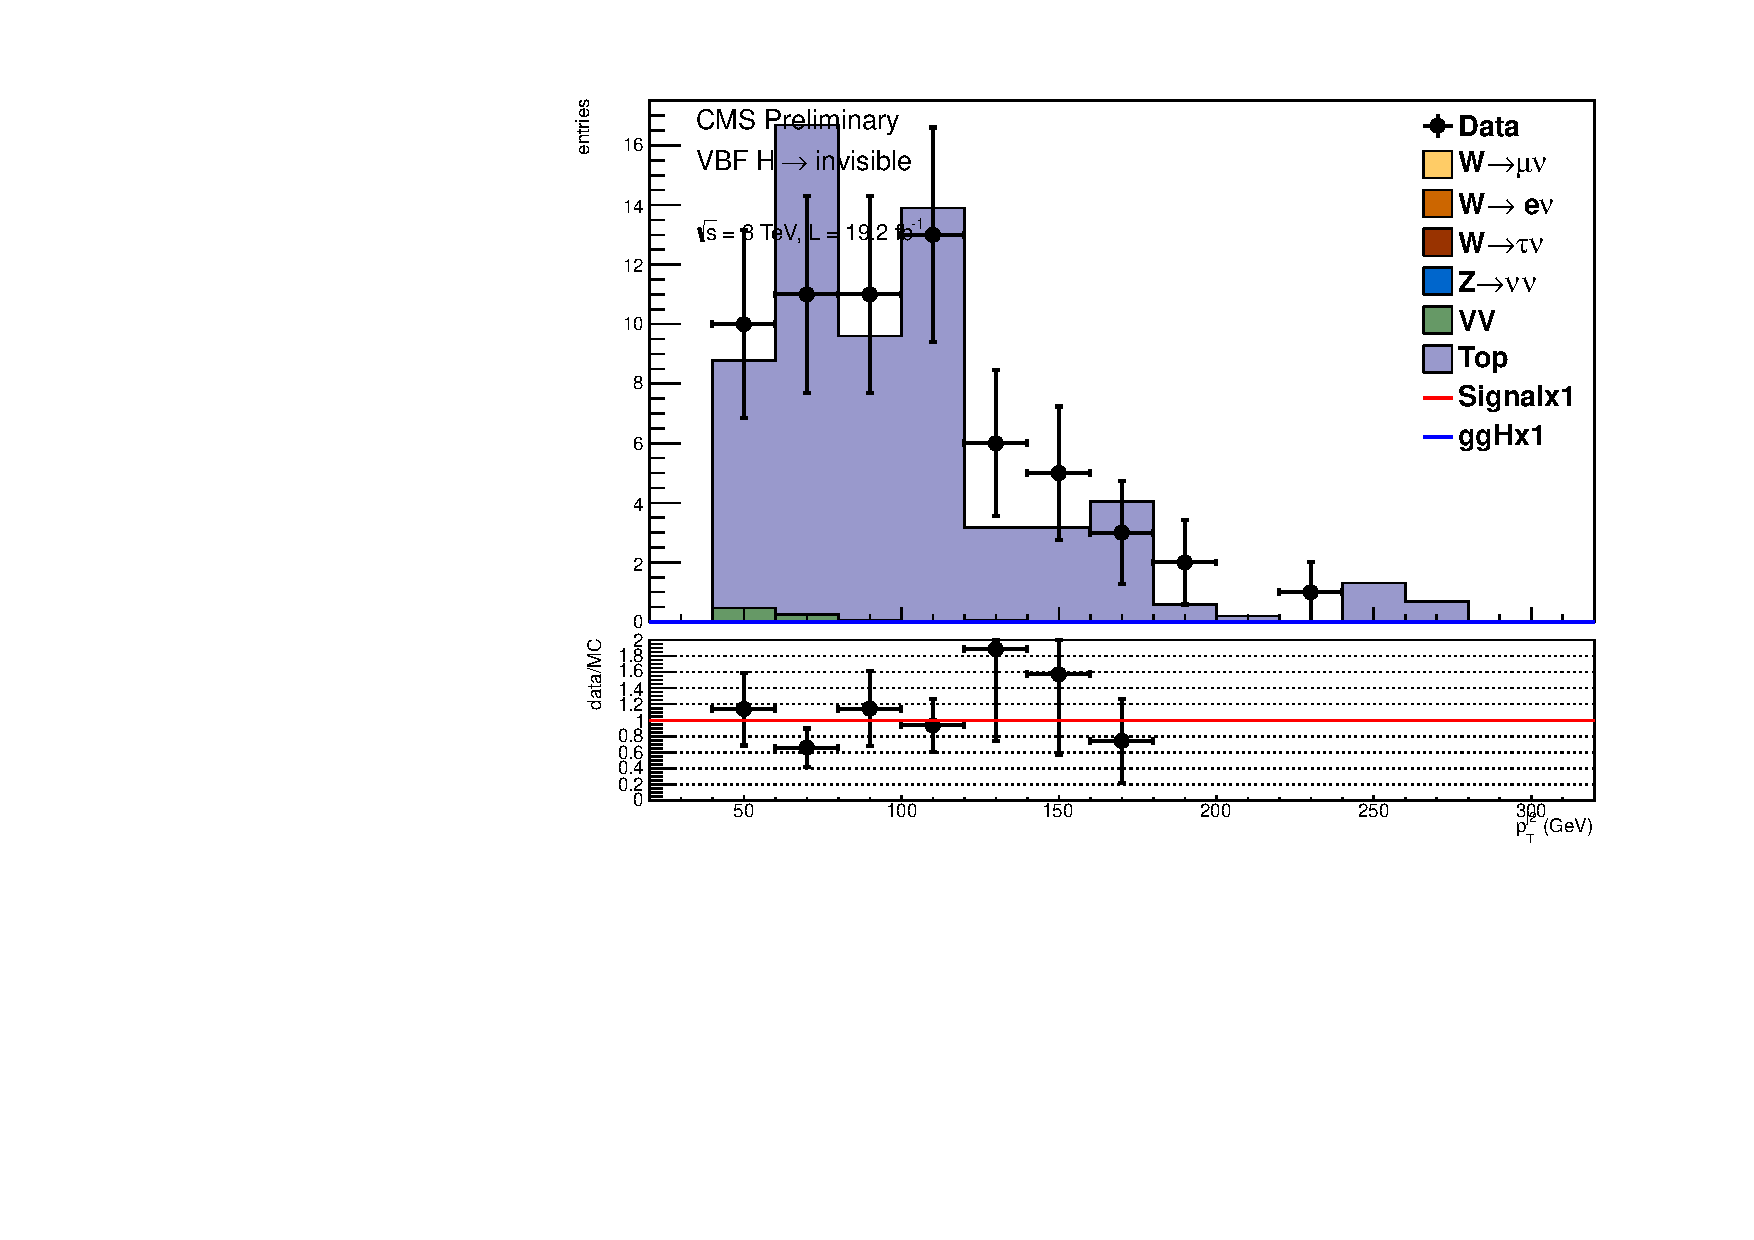
\includegraphics[width=\textwidth]{TalkPics/runcbug101114/output_presel/top_jet2_pt.pdf}
    \end{block}

  \end{columns}
\end{frame}

\begin{frame}
  \frametitle{New control plots - top}
  \begin{columns}
    \column{.5\textwidth}
    \begin{block}{METnomu}
      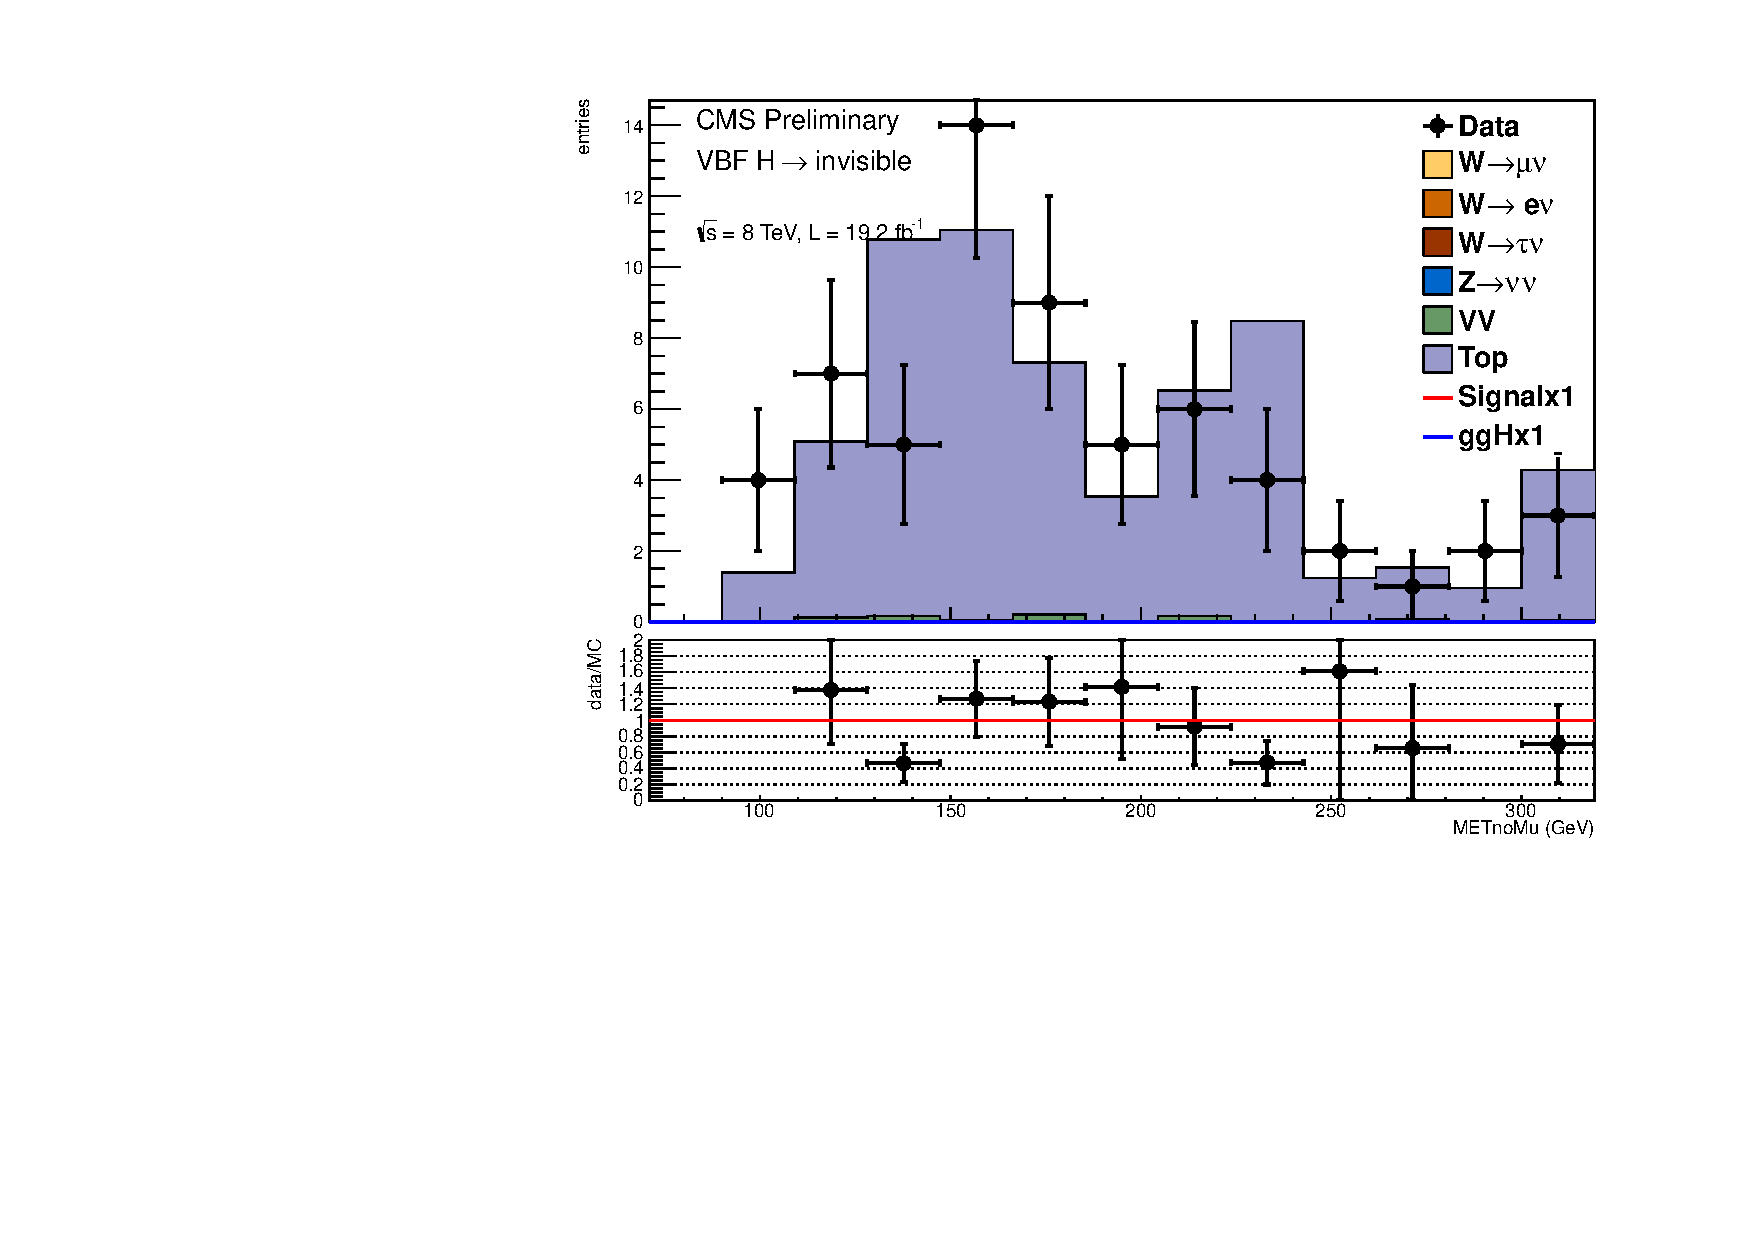
\includegraphics[width=\textwidth]{TalkPics/runcbug101114/output_presel/top_metnomuons.pdf}
    \end{block}
    \column{.5\textwidth}
    \begin{block}{METnomusig}
      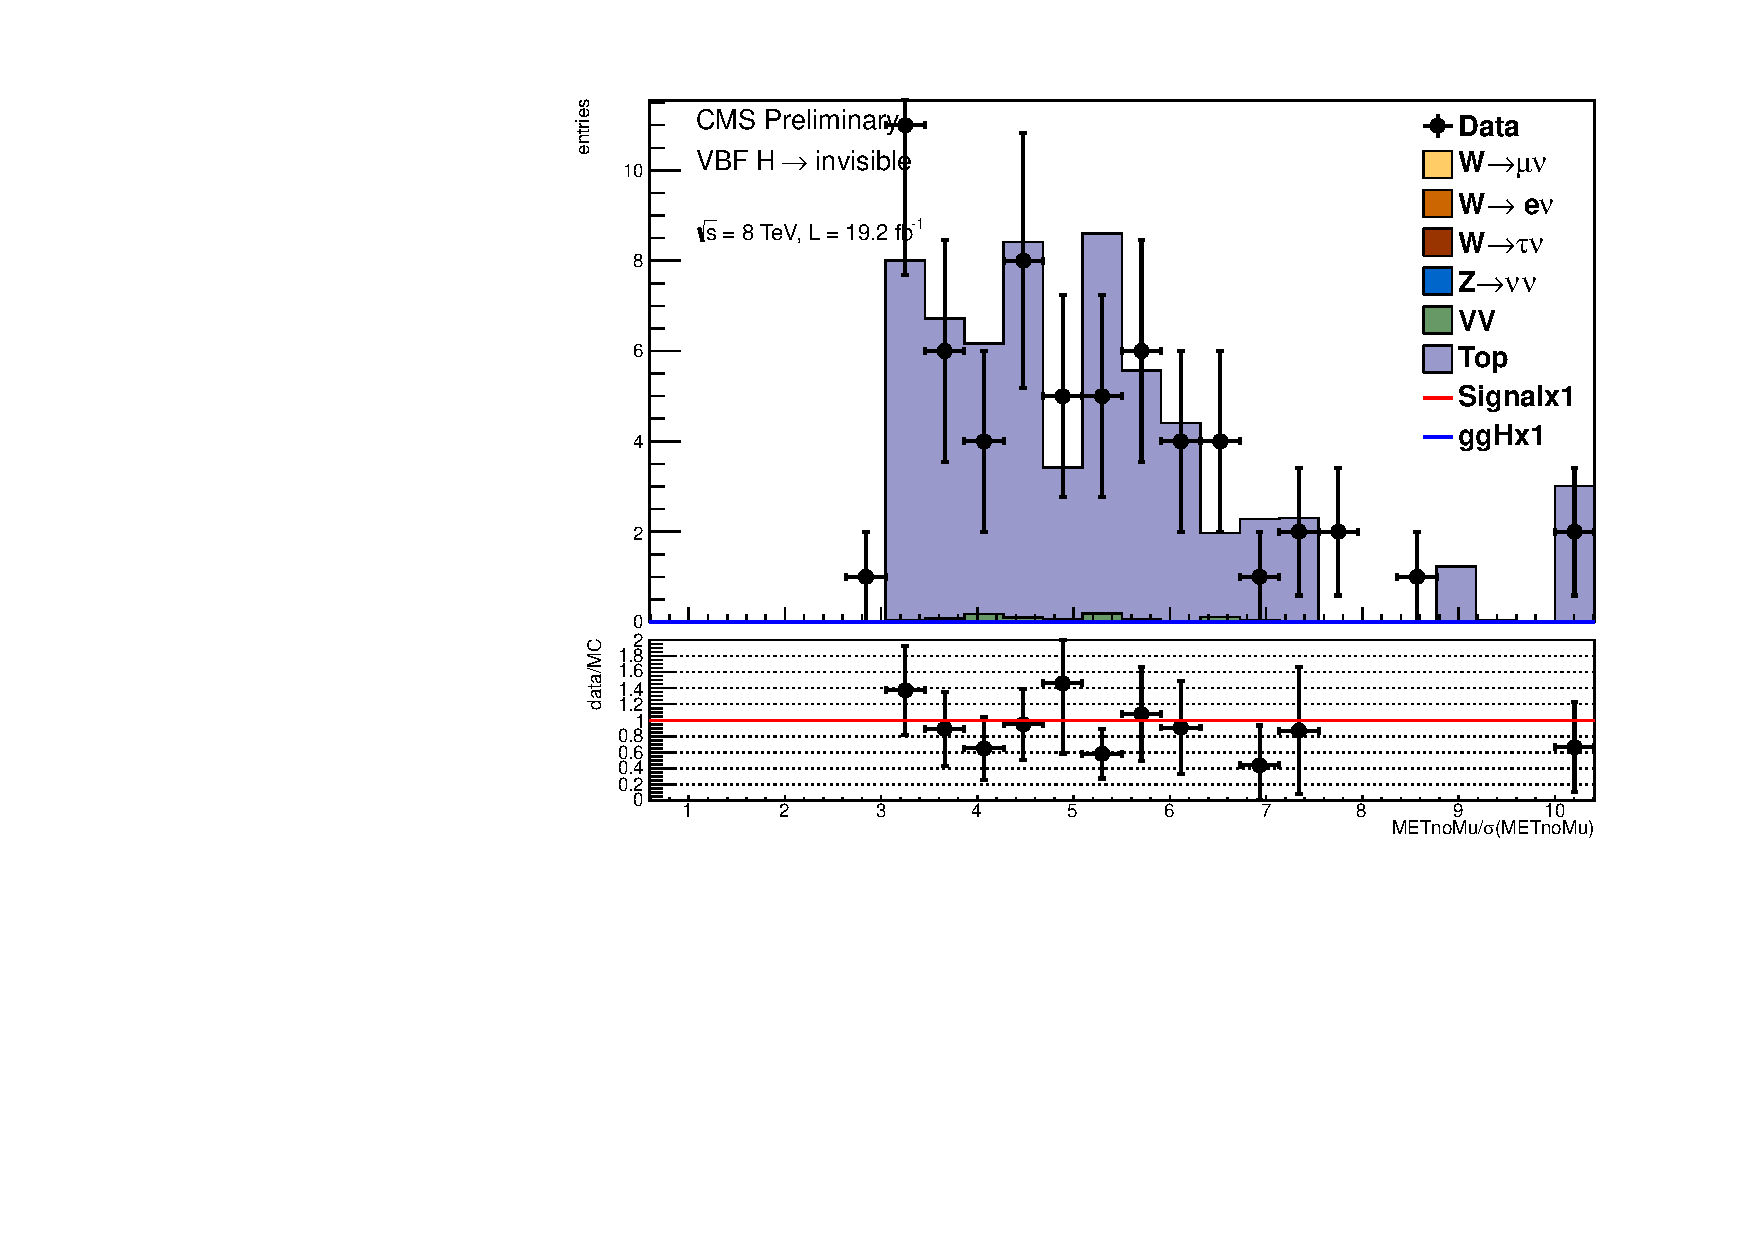
\includegraphics[width=\textwidth]{TalkPics/runcbug101114/output_presel/top_metnomu_significance.pdf}
    \end{block}

  \end{columns}
\end{frame}

\begin{frame}
  \frametitle{New control plots - top }
  \begin{columns}
    \column{.5\textwidth}
    \begin{block}{Mjj}
      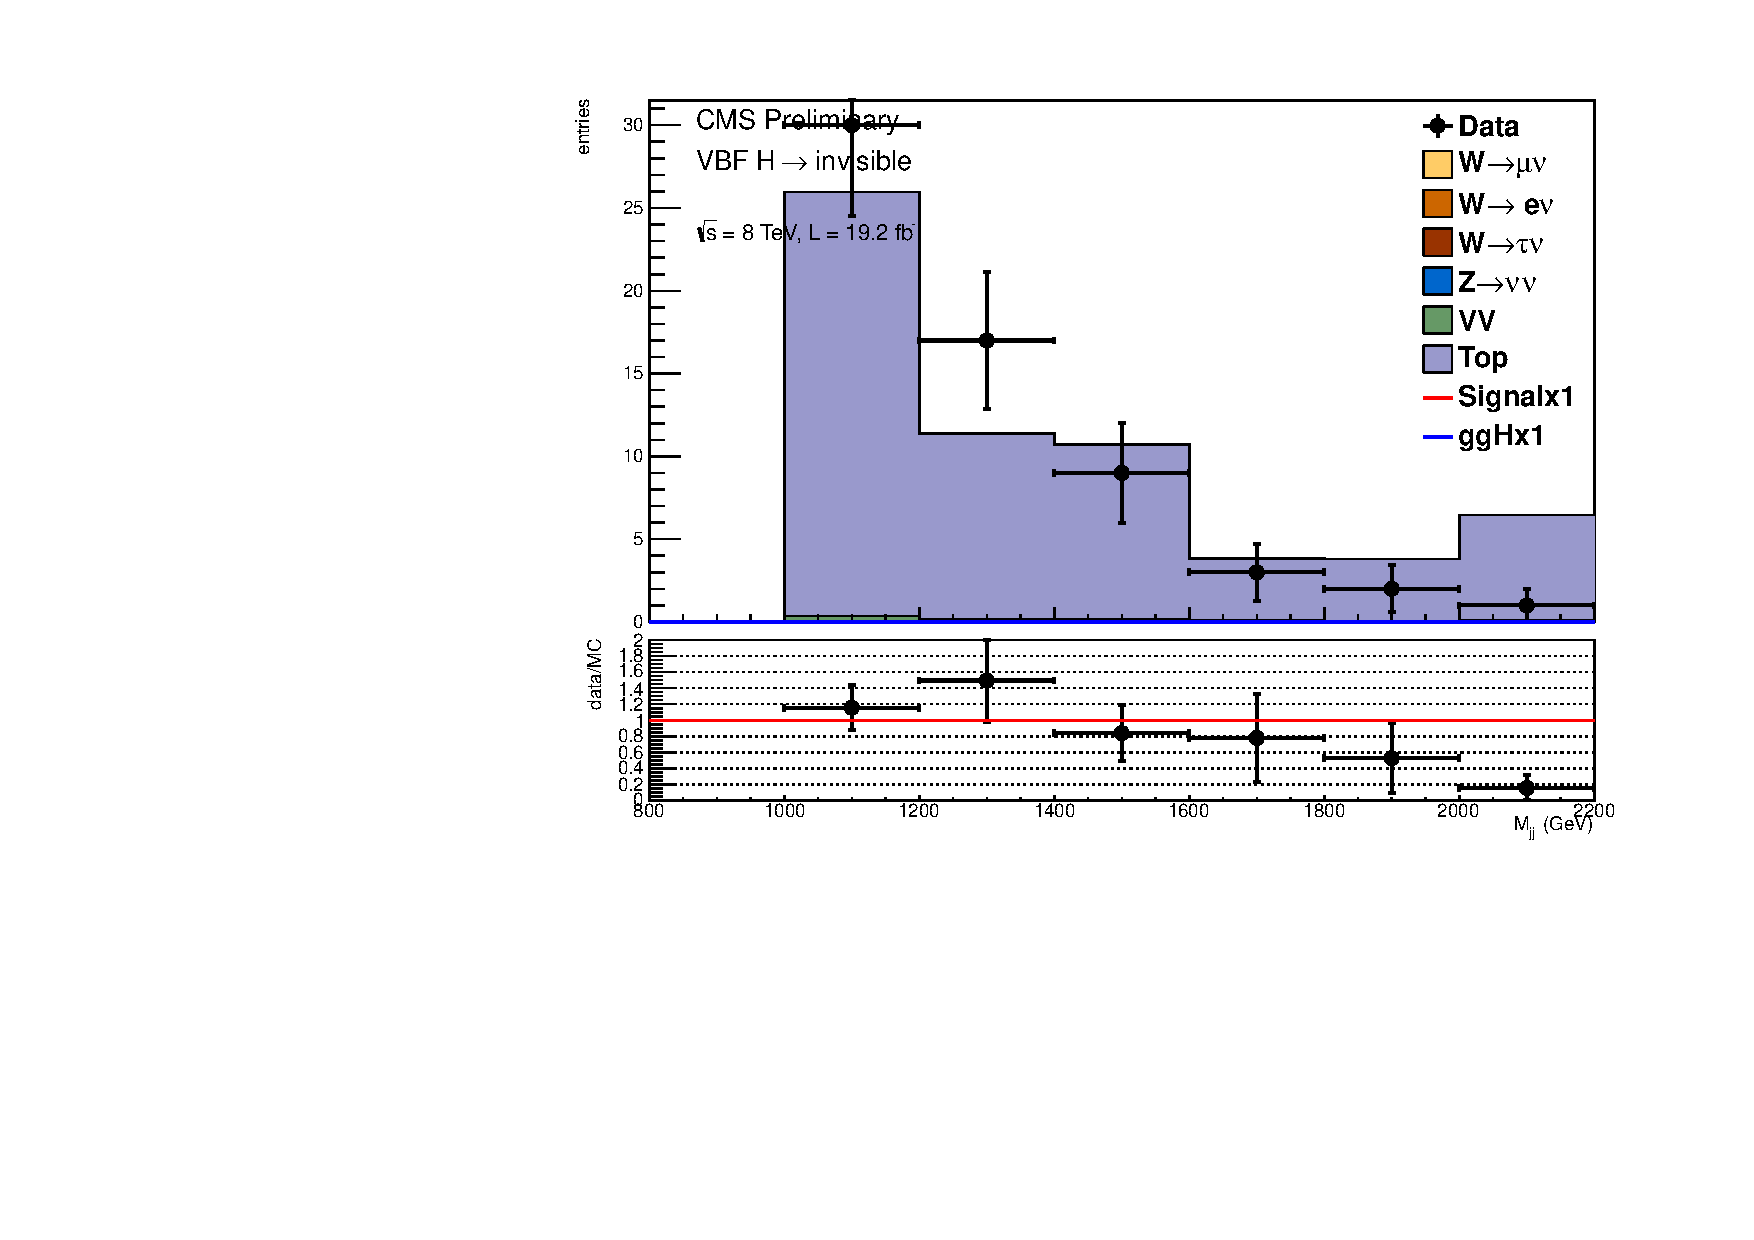
\includegraphics[width=\textwidth]{TalkPics/runcbug101114/output_presel/top_dijet_M.pdf}
    \end{block}
    \column{.5\textwidth}
    \begin{block}{dijet-metnomu pt fraction}
      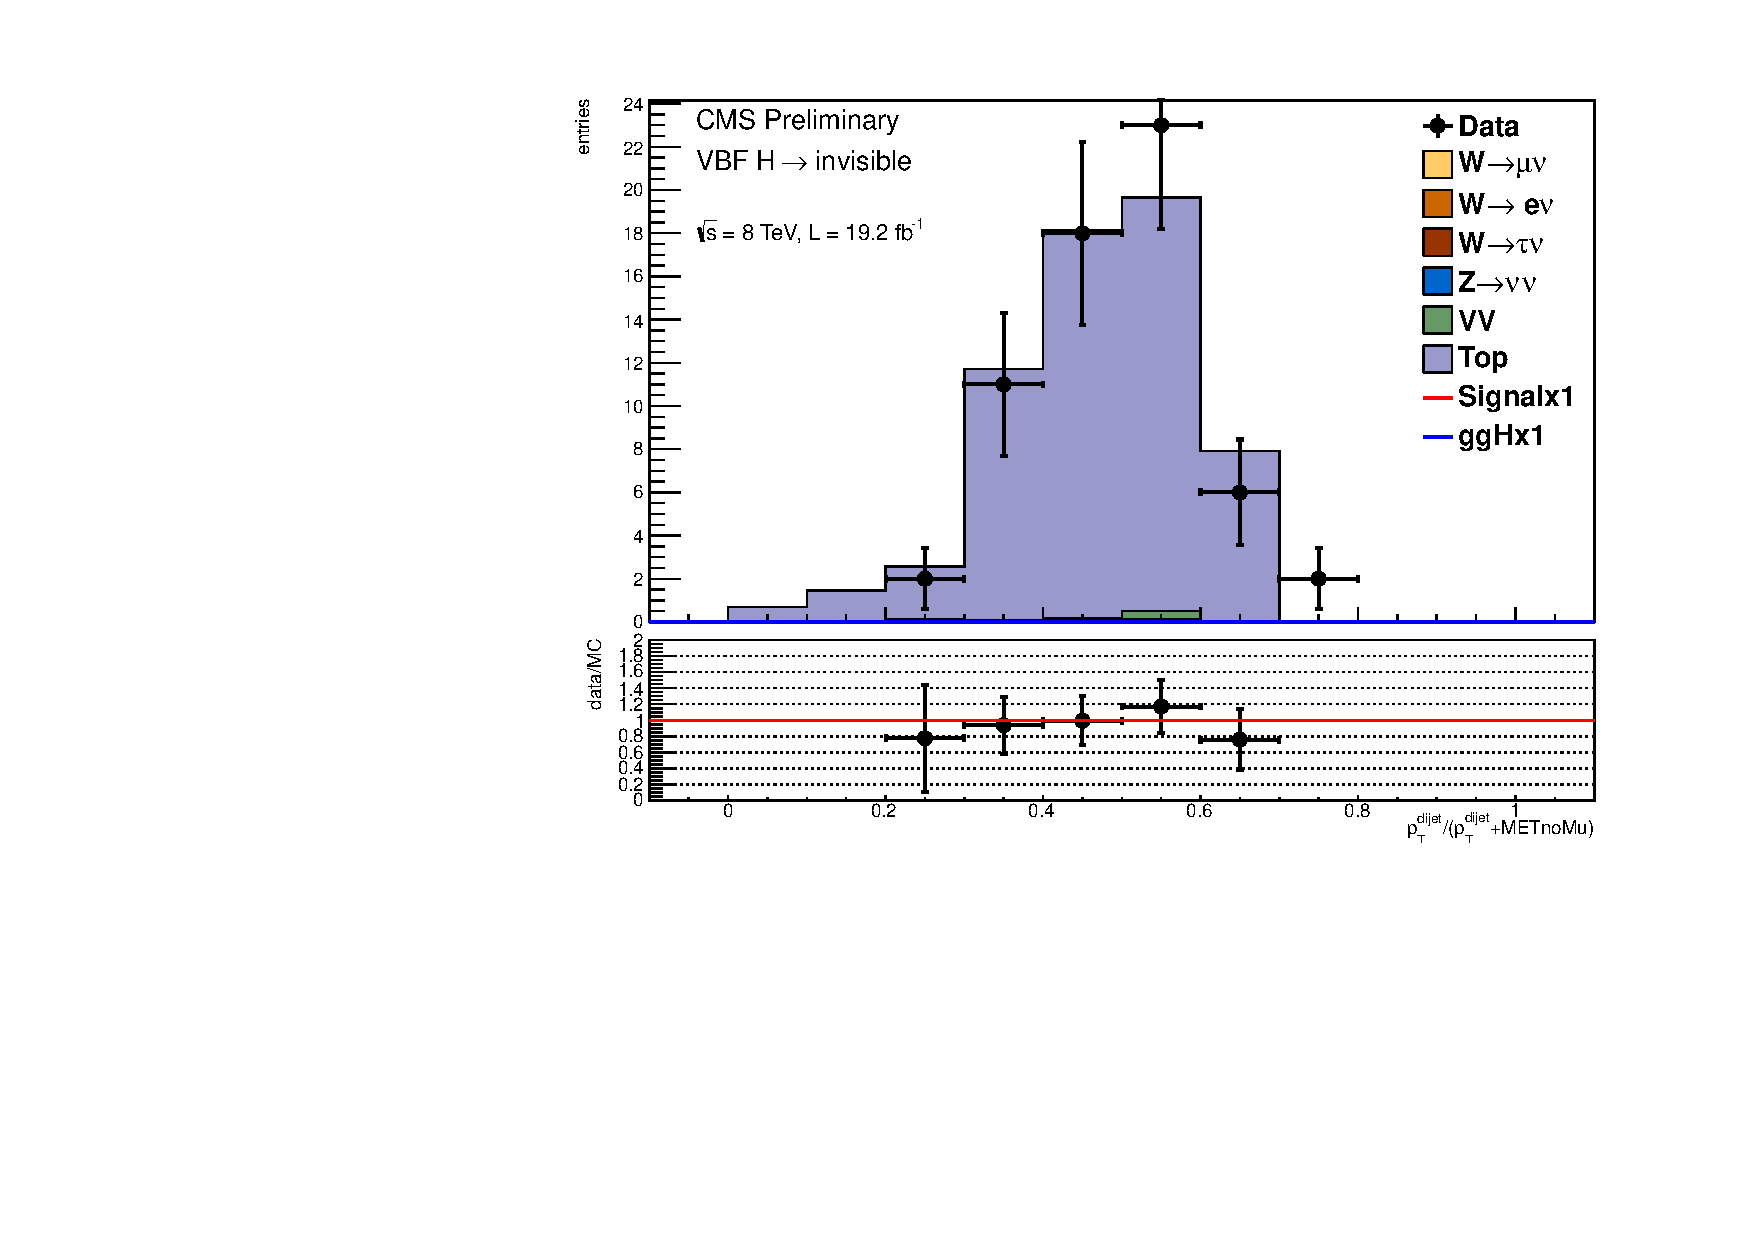
\includegraphics[width=\textwidth]{TalkPics/runcbug101114/output_presel/top_dijetmetnomu_ptfraction.pdf}
    \end{block}
  \end{columns}
\end{frame}

\begin{frame}
  \frametitle{New control plots -top}
  \begin{columns}
    \column{.5\textwidth}
    \begin{block}{Dphijj}
      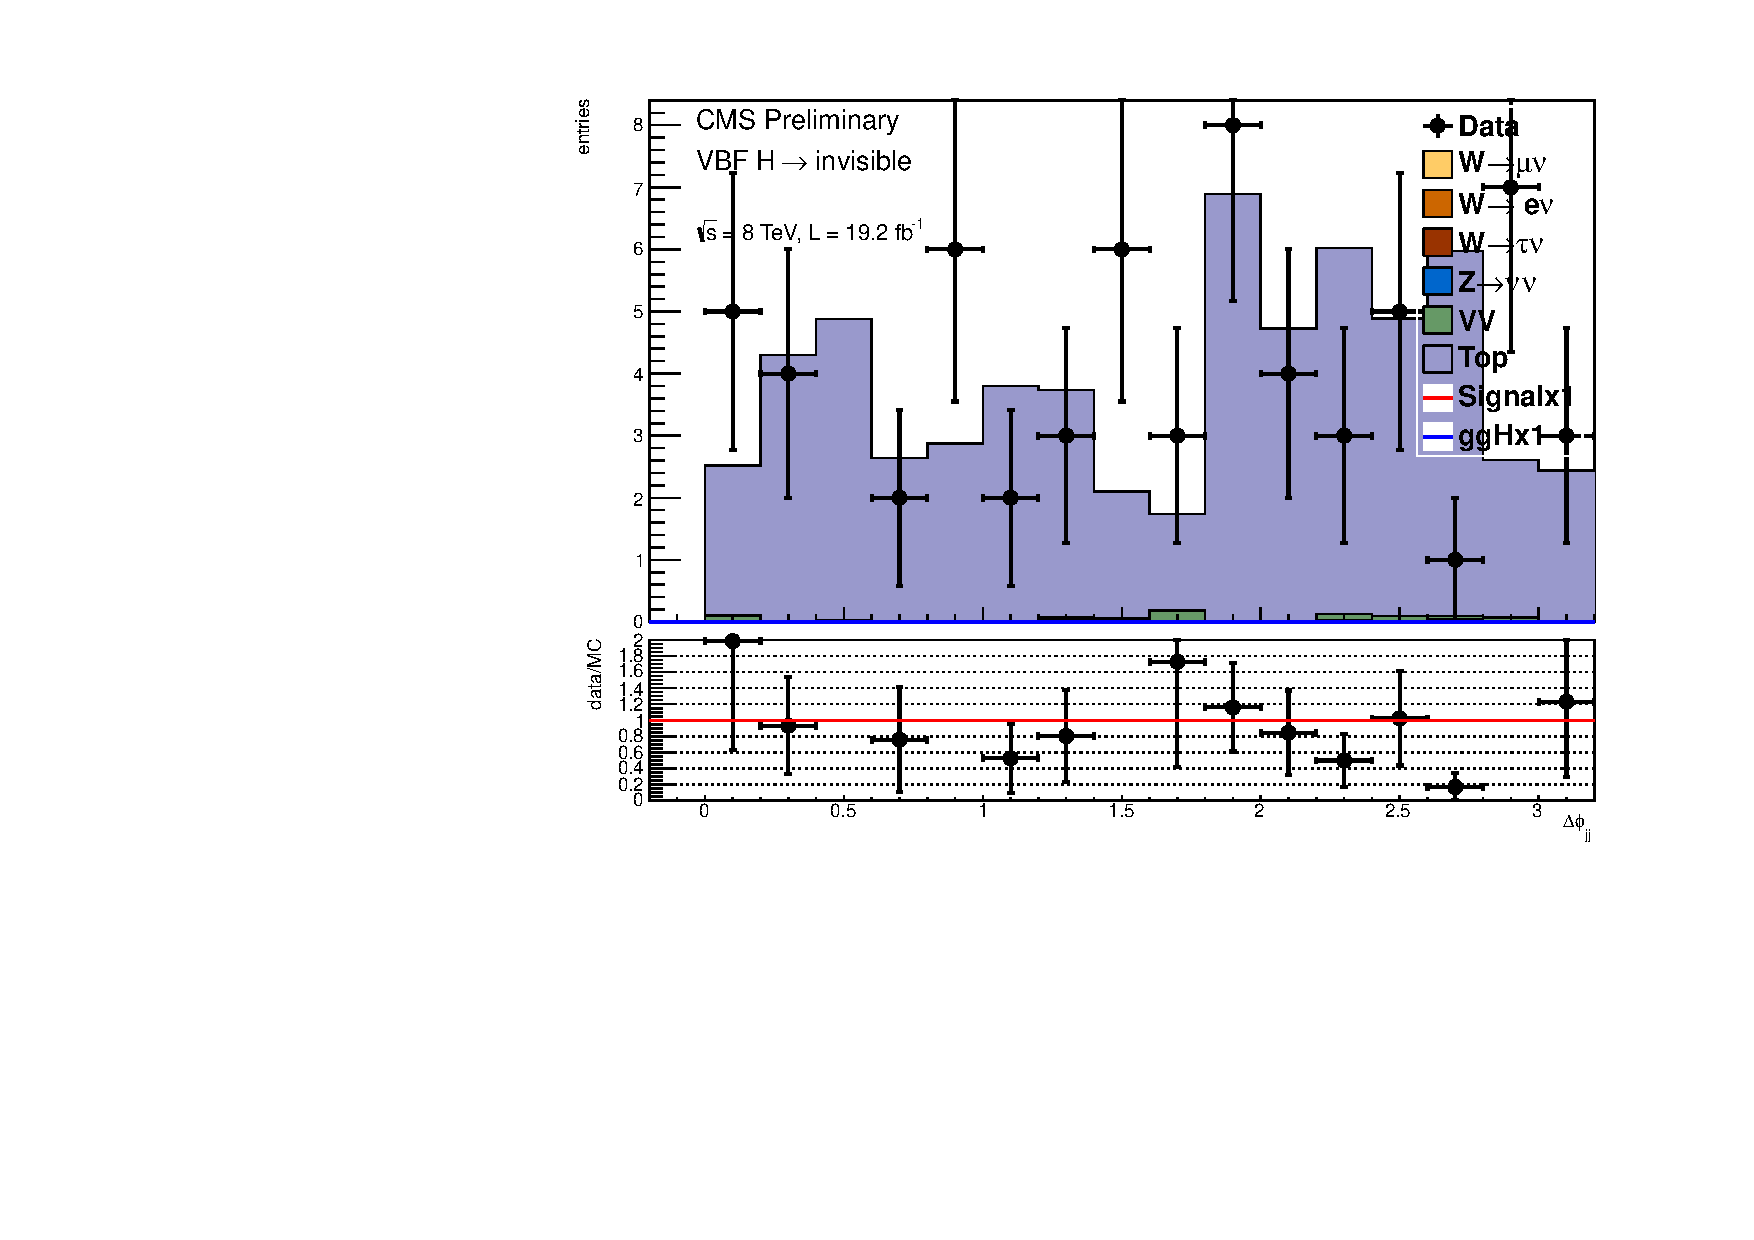
\includegraphics[width=\textwidth]{TalkPics/runcbug101114/output_presel/top_dijet_dphi.pdf}
    \end{block}
    \column{.5\textwidth}
    \begin{block}{Detajj}
      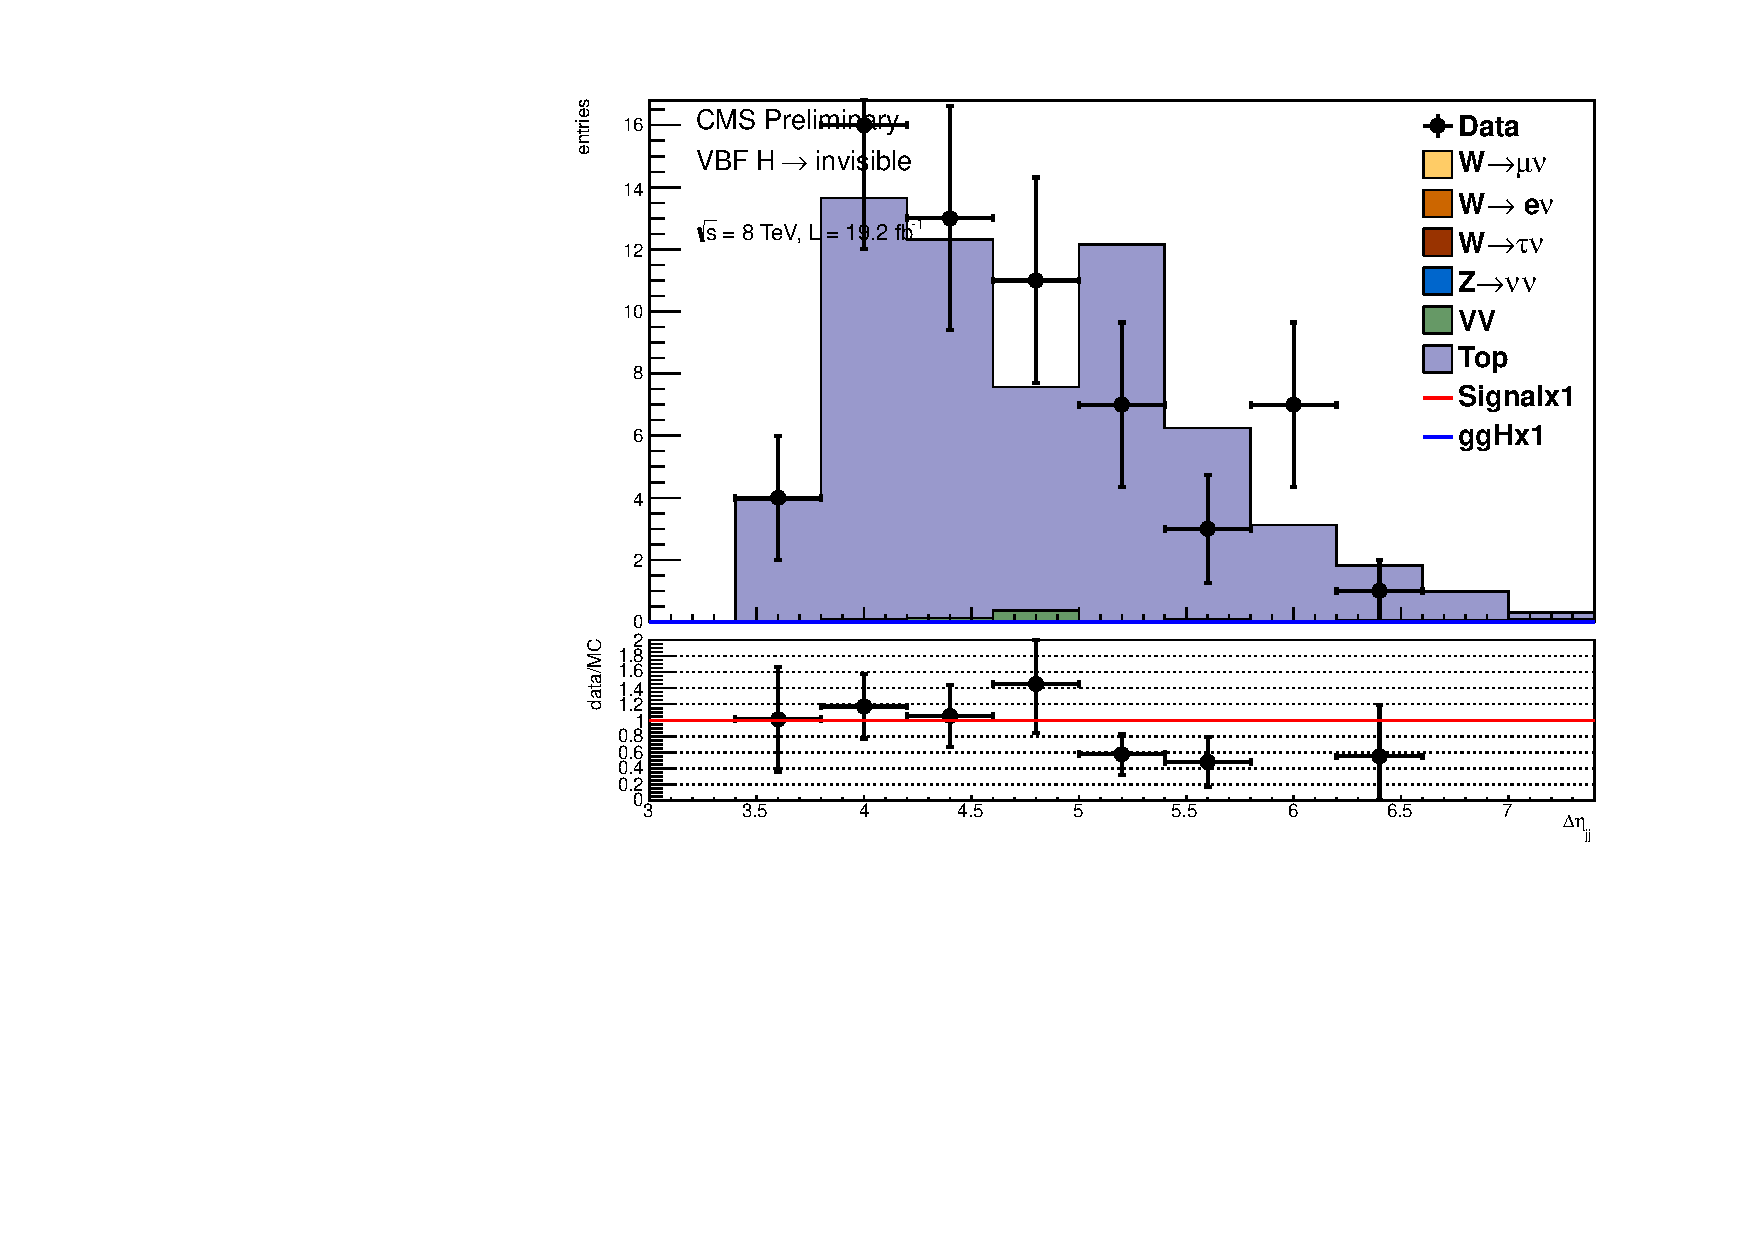
\includegraphics[width=\textwidth]{TalkPics/runcbug101114/output_presel/top_dijet_deta.pdf}
    \end{block}

  \end{columns}
\end{frame}

\begin{frame}
  \frametitle{New control plots -top}
  \begin{columns}
    \column{.5\textwidth}
    \begin{block}{Leading jets-met mindphi}
      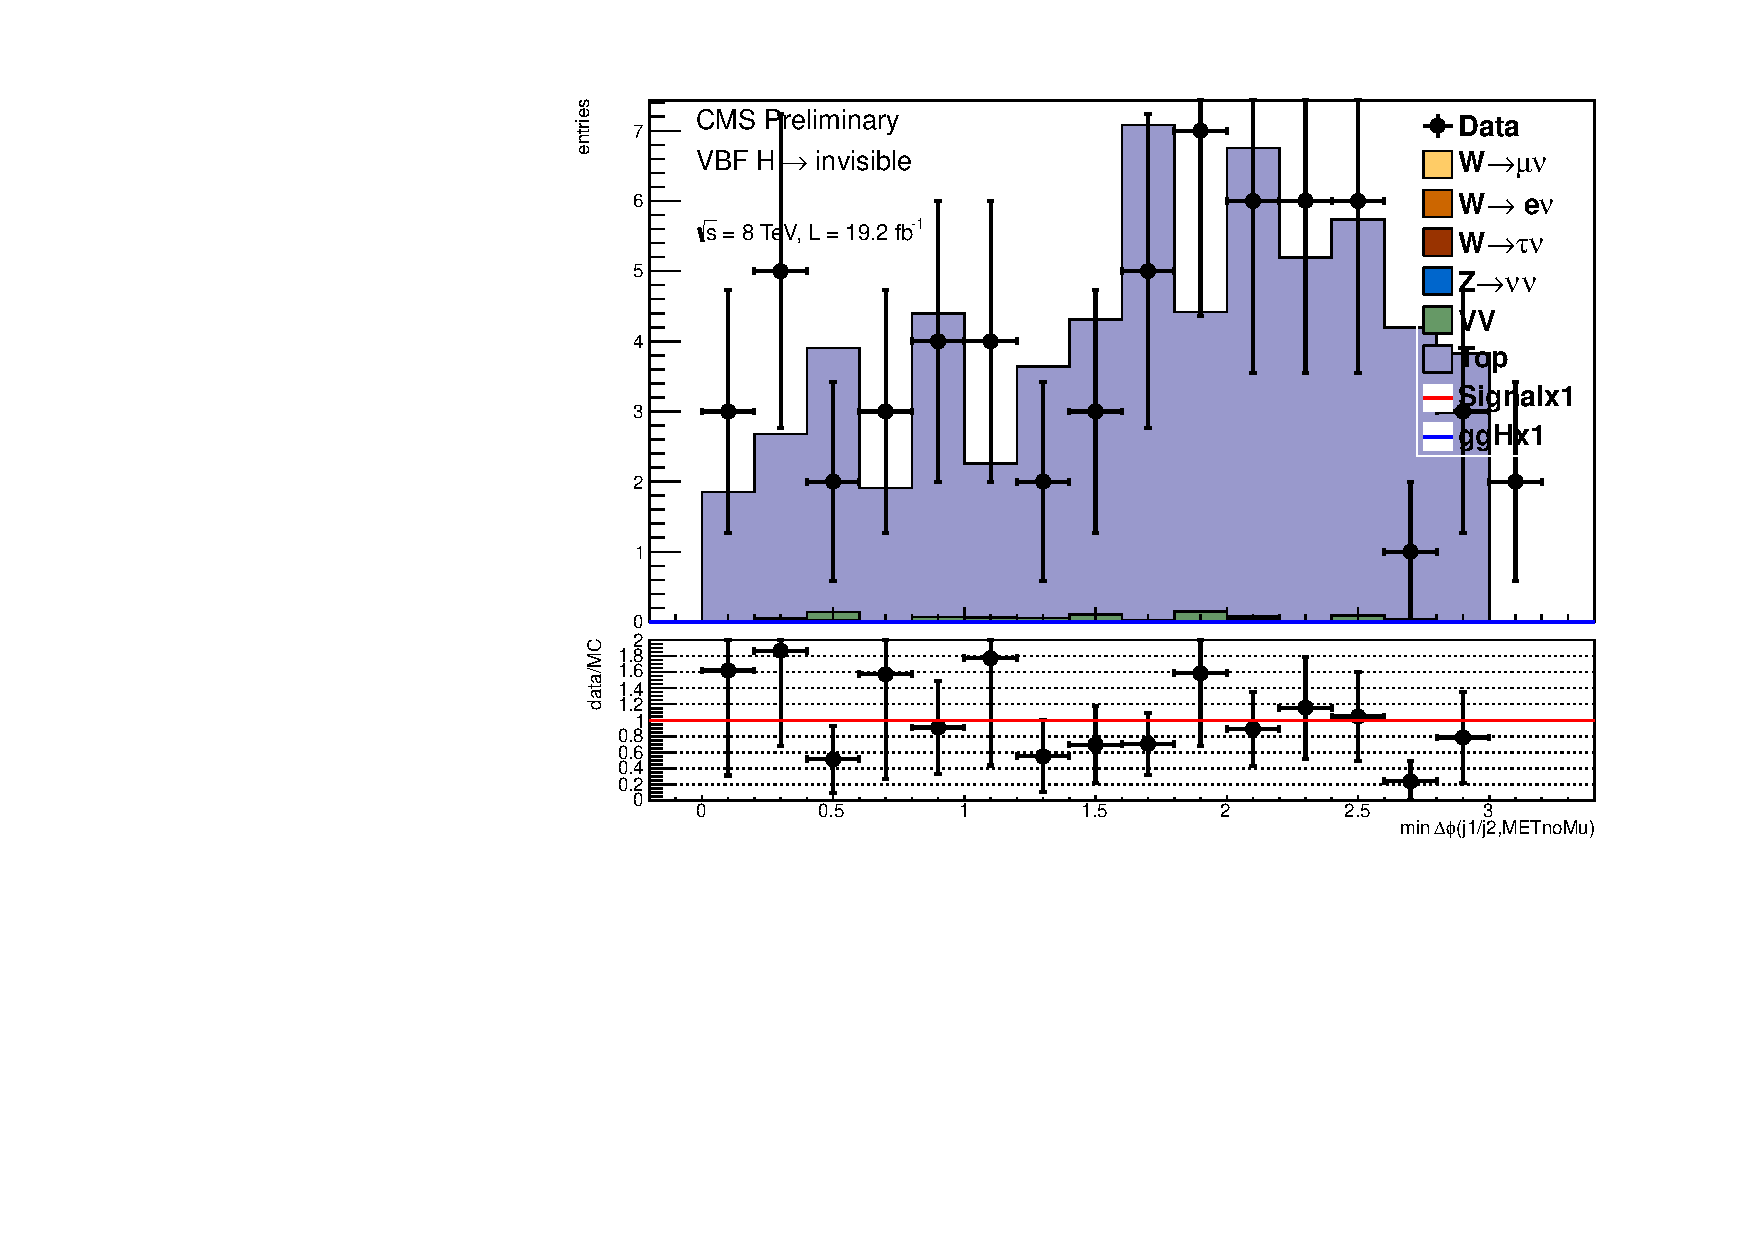
\includegraphics[width=\textwidth]{TalkPics/runcbug101114/output_presel/top_jetmetnomu_mindphi.pdf}
    \end{block}
    \column{.5\textwidth}
    \begin{block}{All jet-met mindphi}
      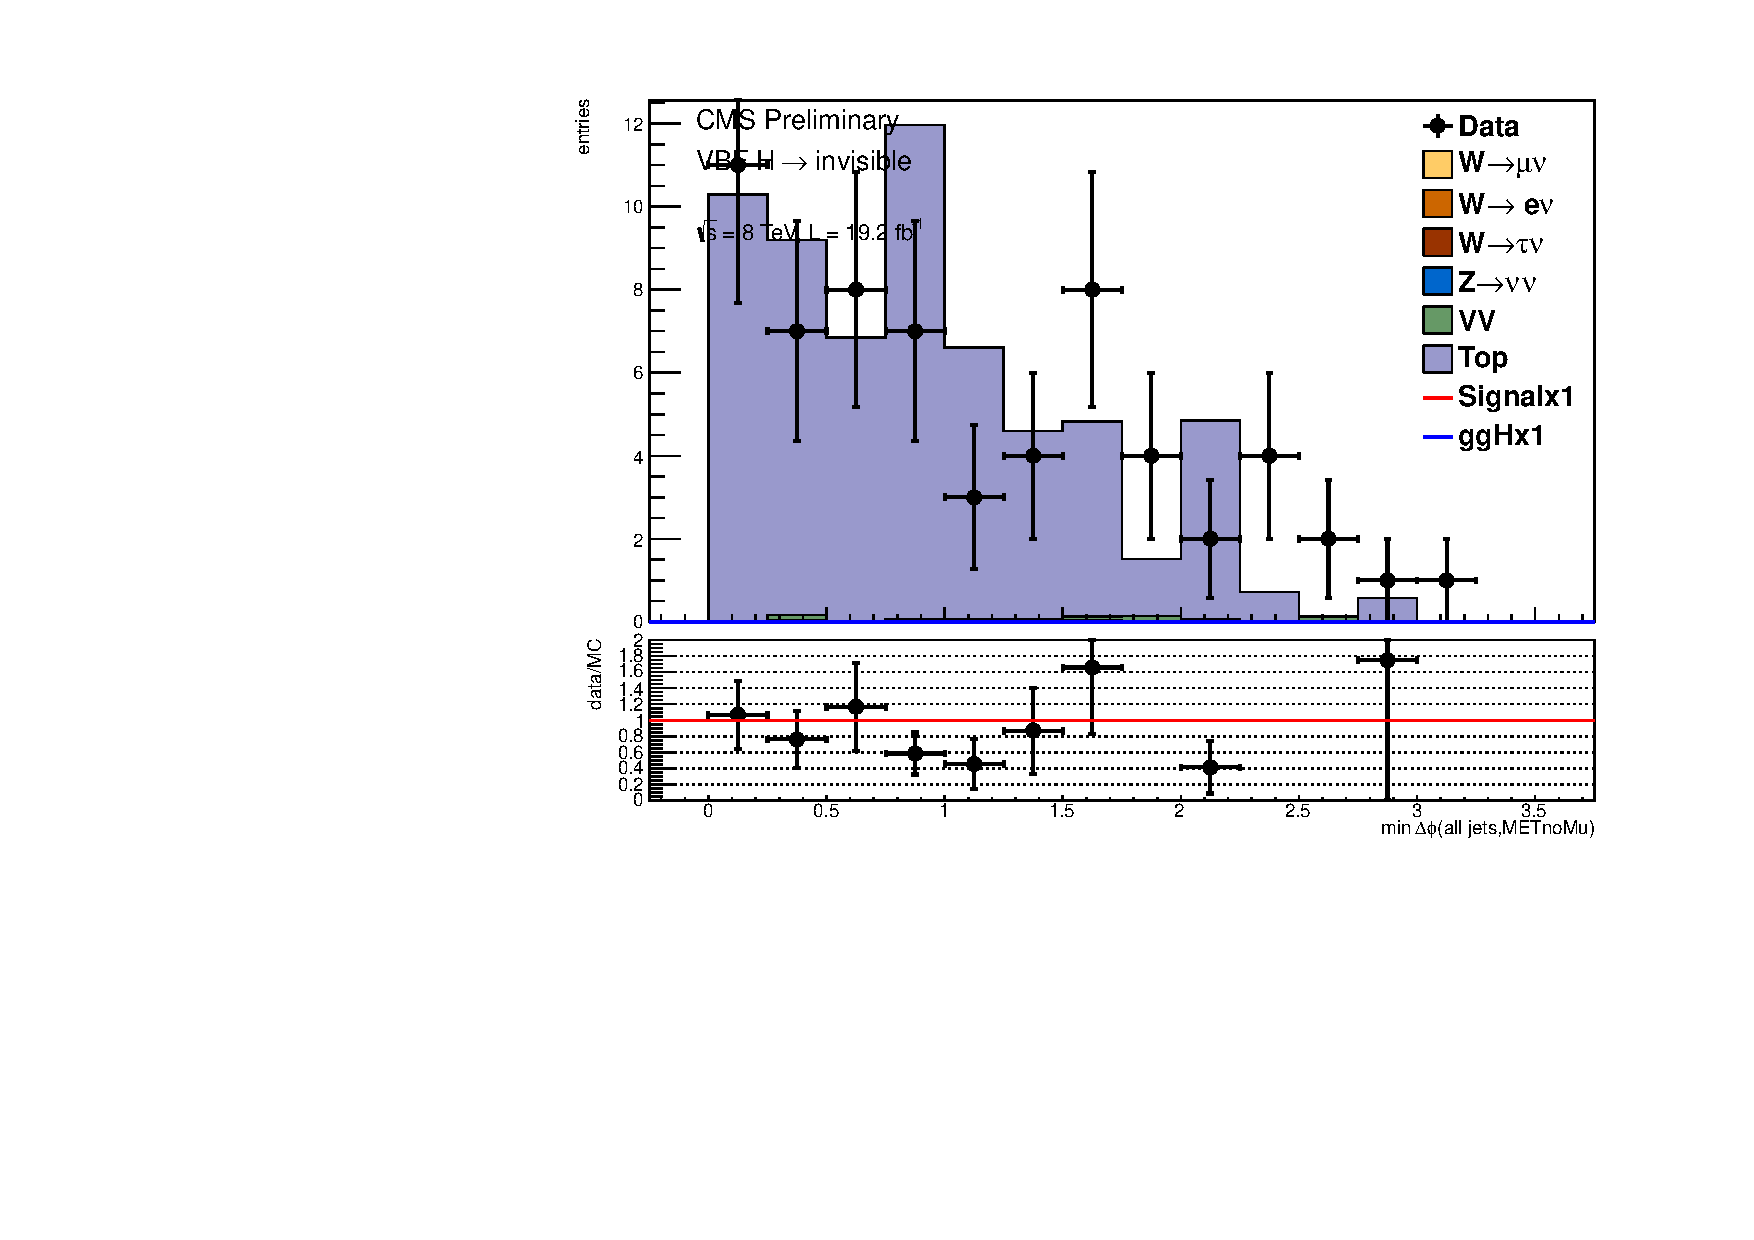
\includegraphics[width=\textwidth]{TalkPics/runcbug101114/output_presel/top_alljetsmetnomu_mindphi.pdf}
    \end{block}

  \end{columns}
\end{frame}

\begin{frame}
  \frametitle{New control plots -enu}
  \begin{columns}
    \column{.5\textwidth}
    \begin{block}{Jet 1 pt}
      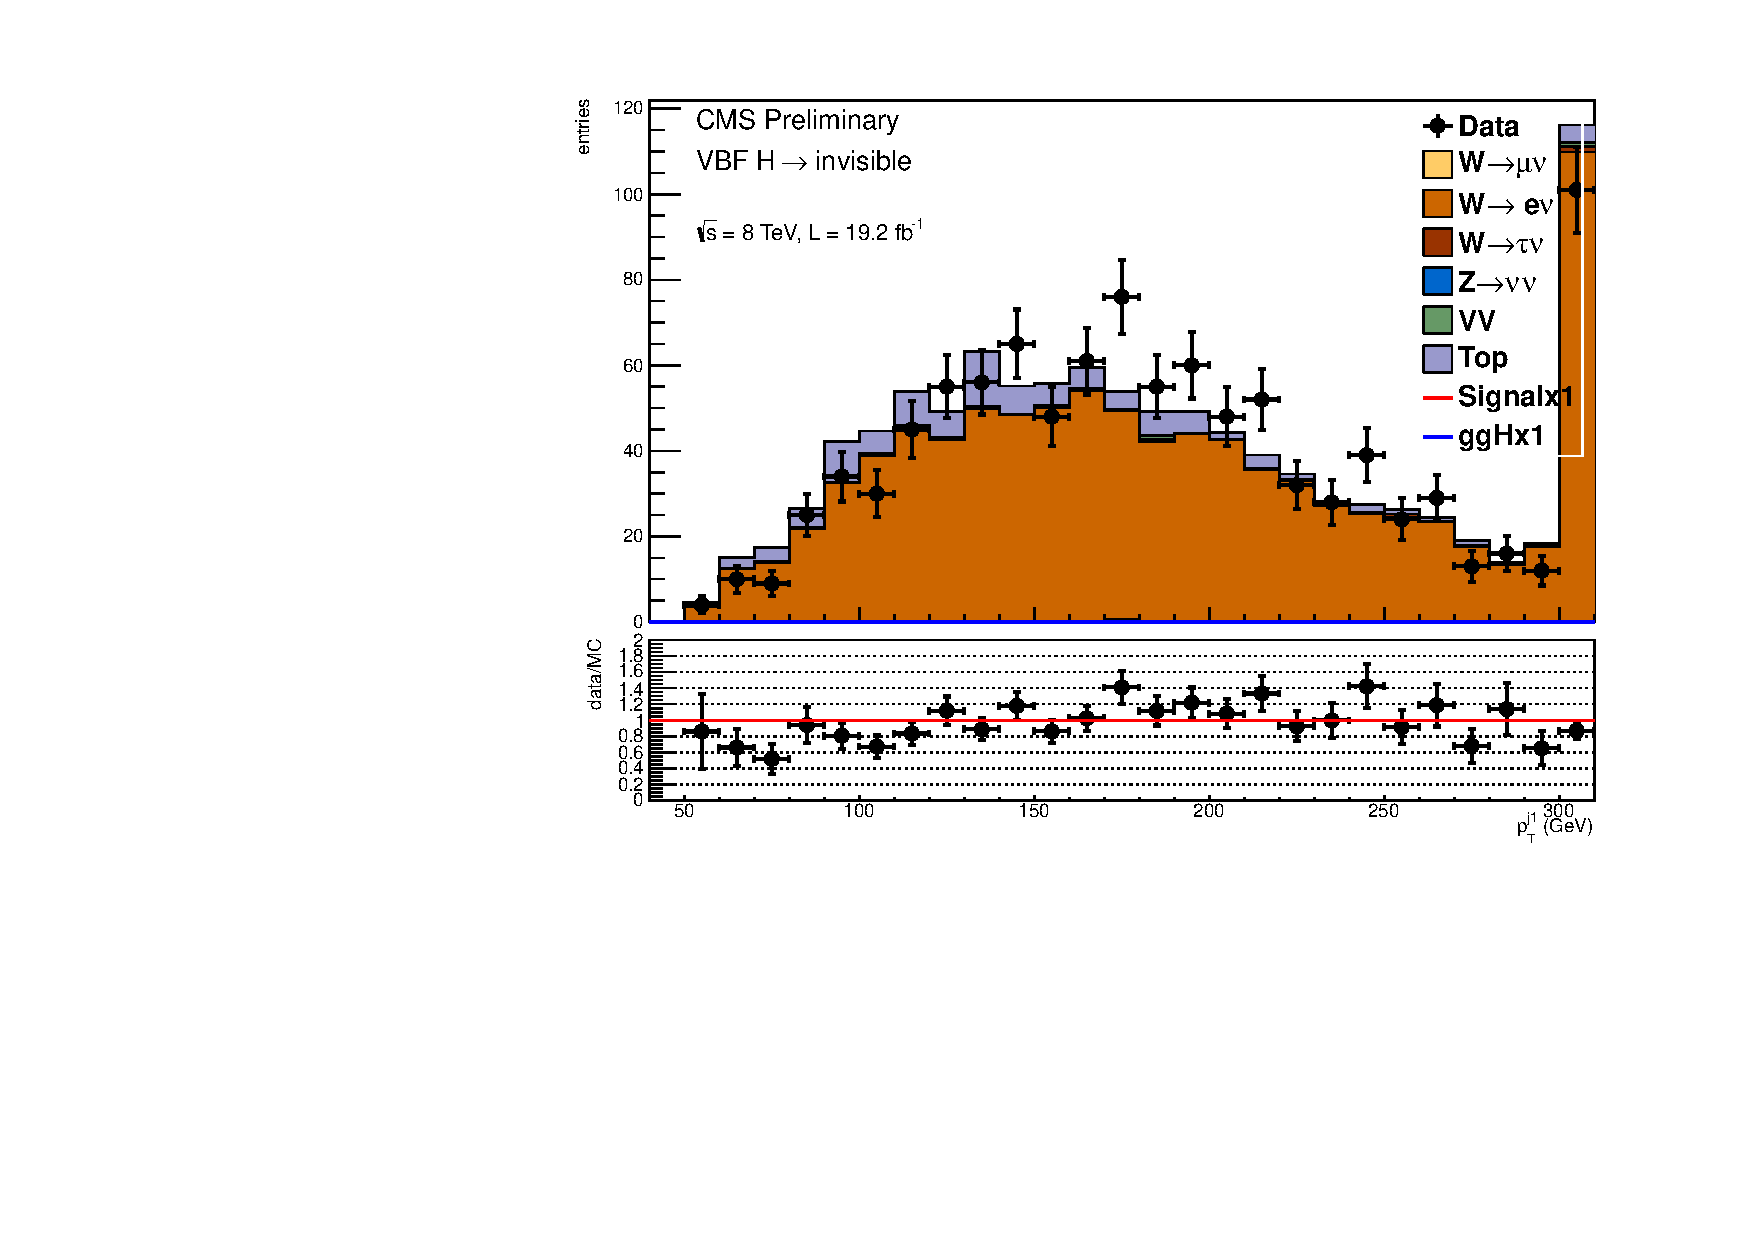
\includegraphics[width=\textwidth]{TalkPics/runcbug101114/output_presel/enu_jet1_pt.pdf}
    \end{block}
    \column{.5\textwidth}
    \begin{block}{Jet 2 pt}
      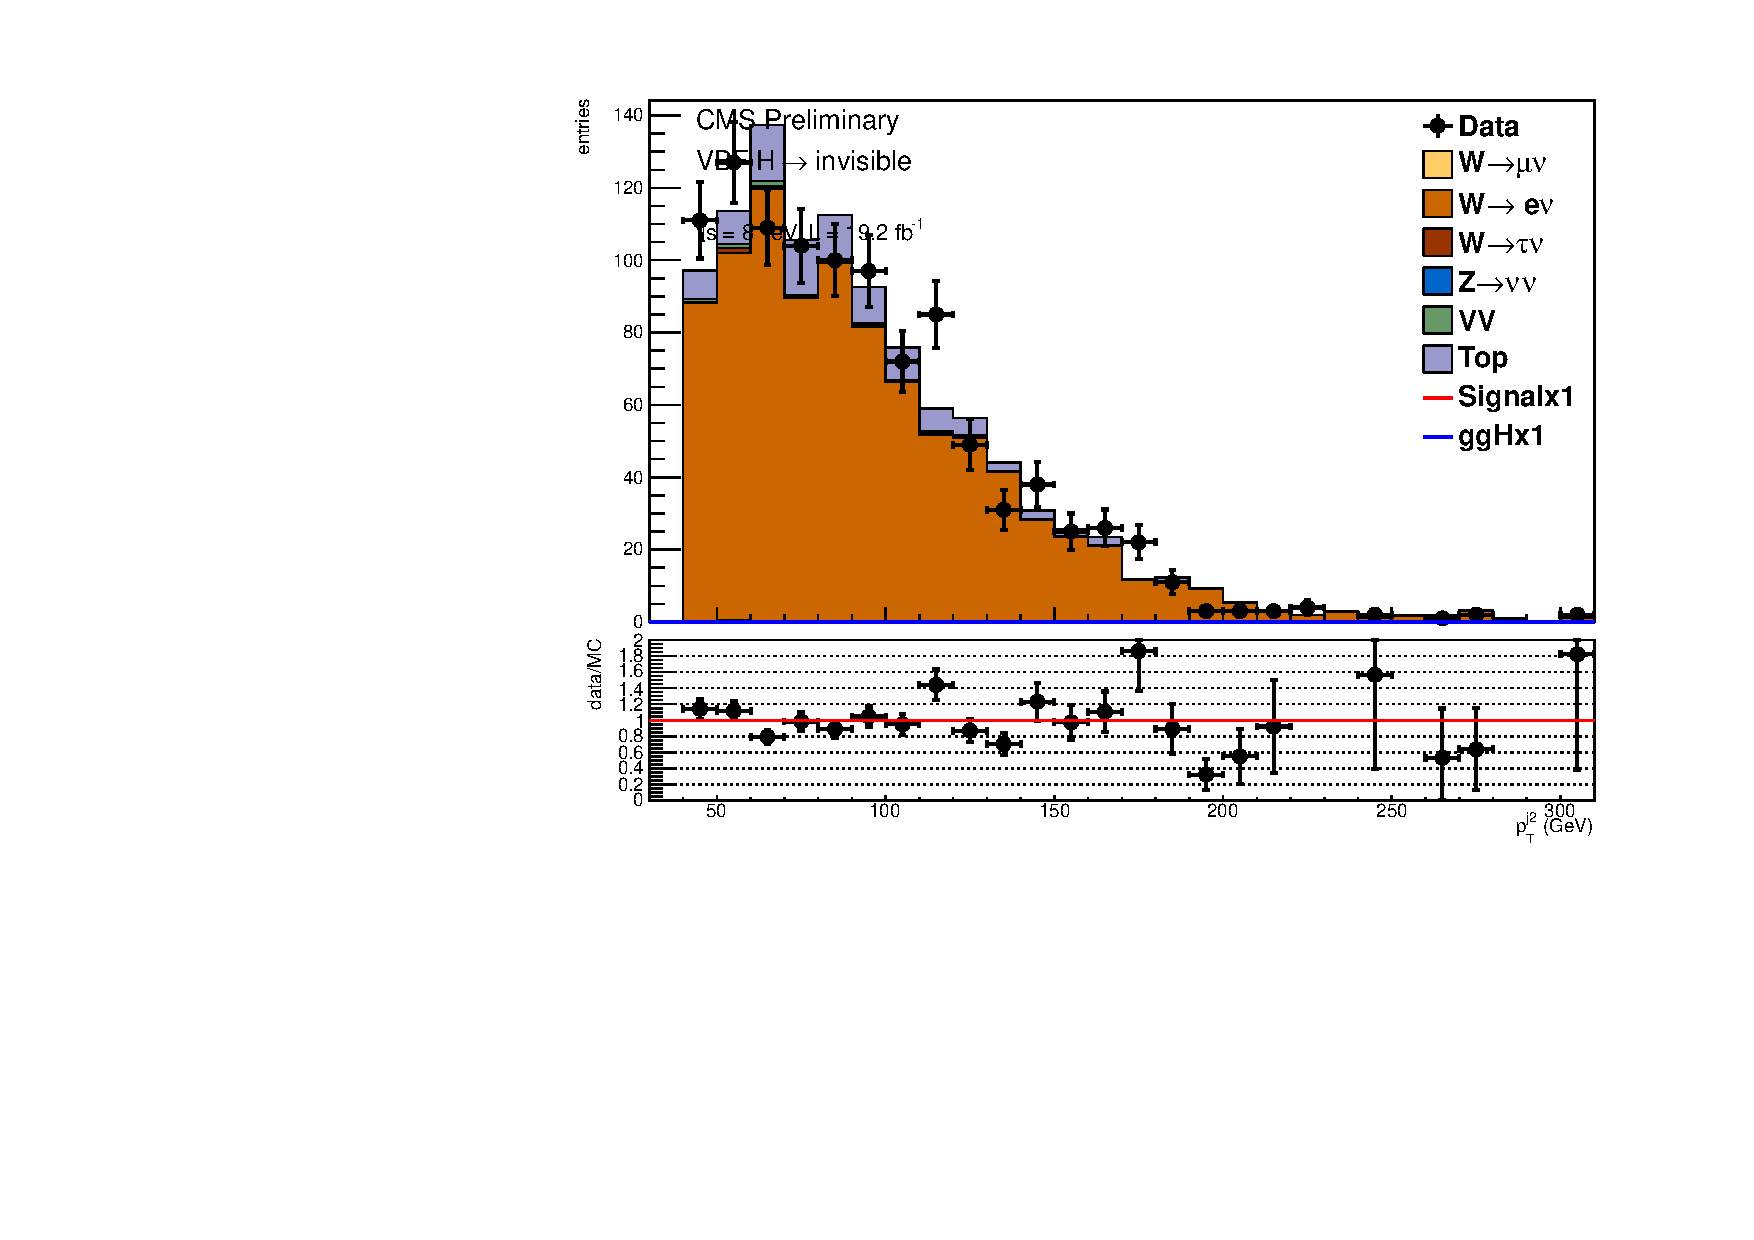
\includegraphics[width=\textwidth]{TalkPics/runcbug101114/output_presel/enu_jet2_pt.pdf}
    \end{block}

  \end{columns}
\end{frame}

\begin{frame}
  \frametitle{New control plots -enu}
  \begin{columns}
    \column{.5\textwidth}
    \begin{block}{METnomu}
      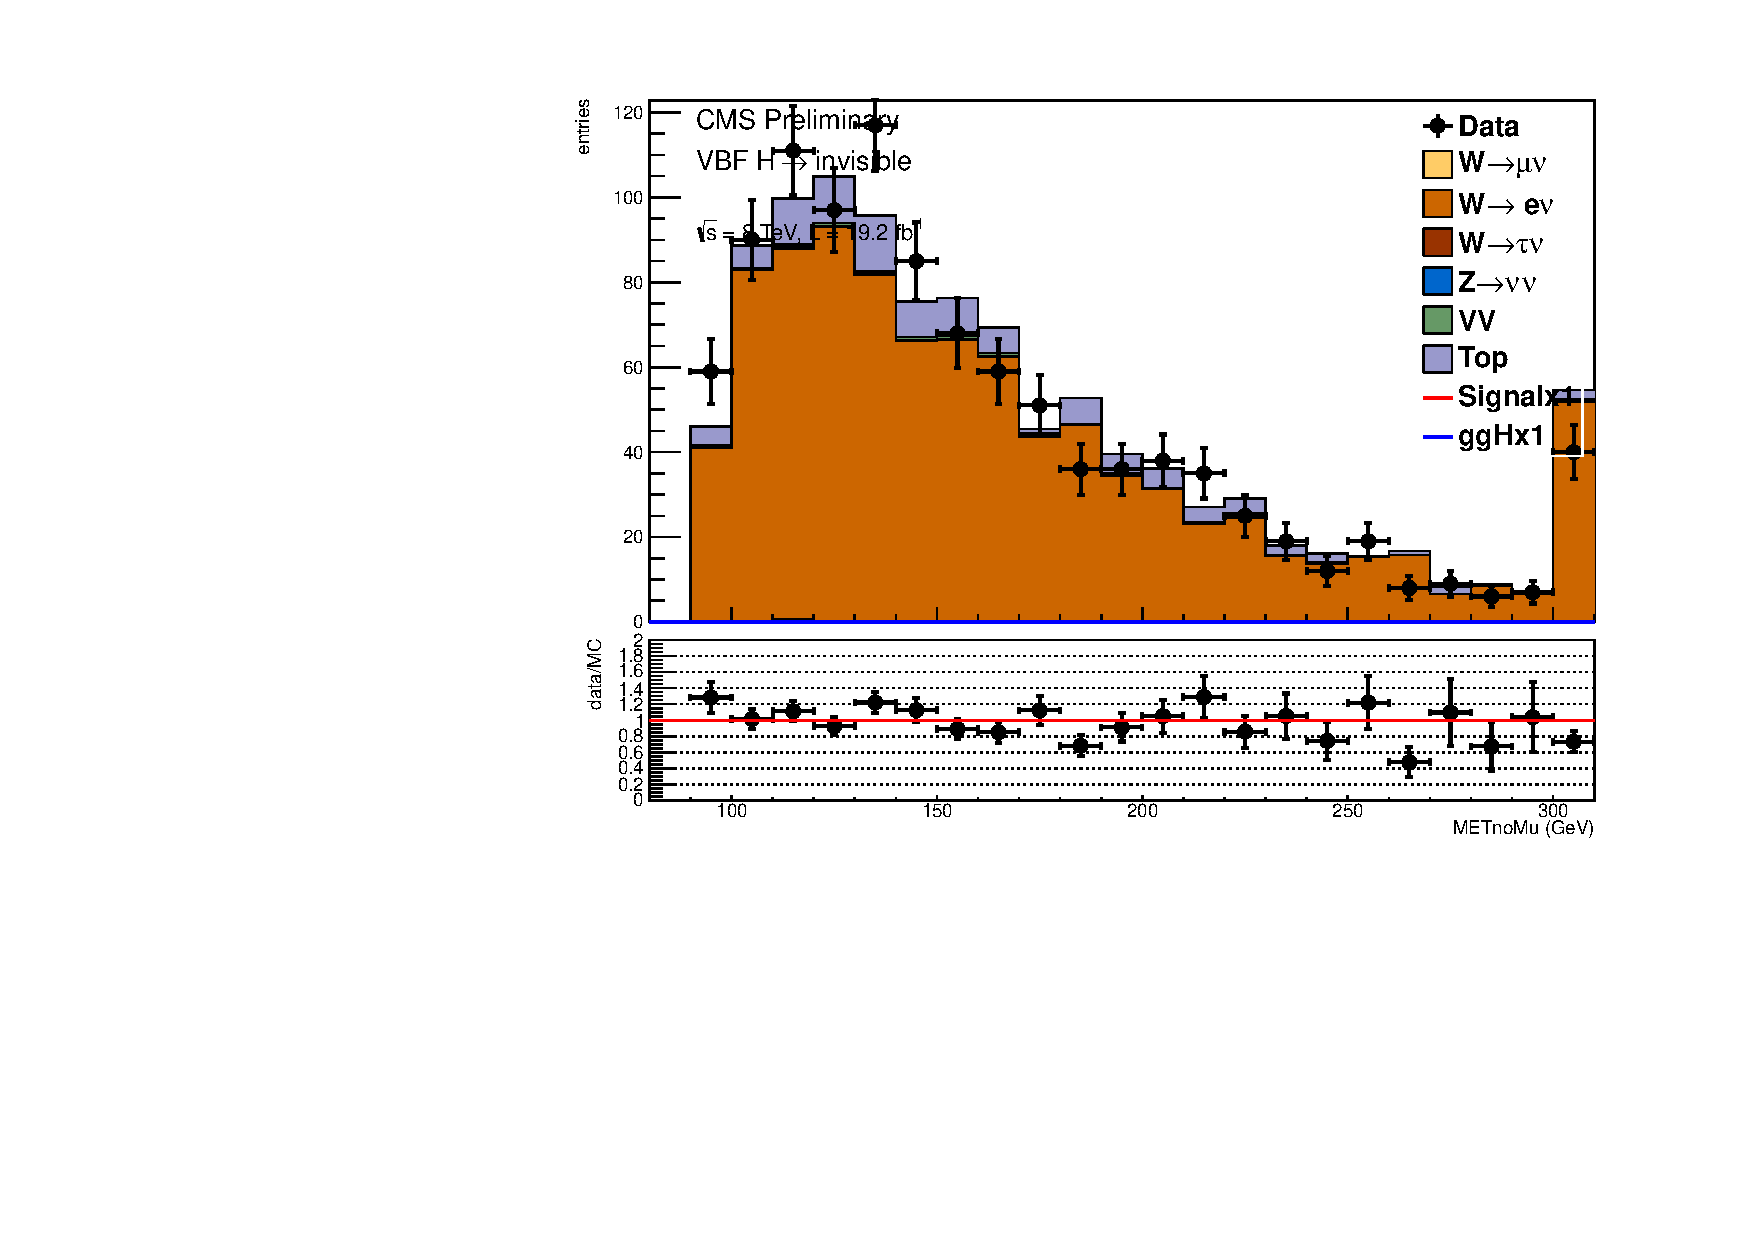
\includegraphics[width=\textwidth]{TalkPics/runcbug101114/output_presel/enu_metnomuons.pdf}
    \end{block}
    \column{.5\textwidth}
    \begin{block}{METnomusig}
      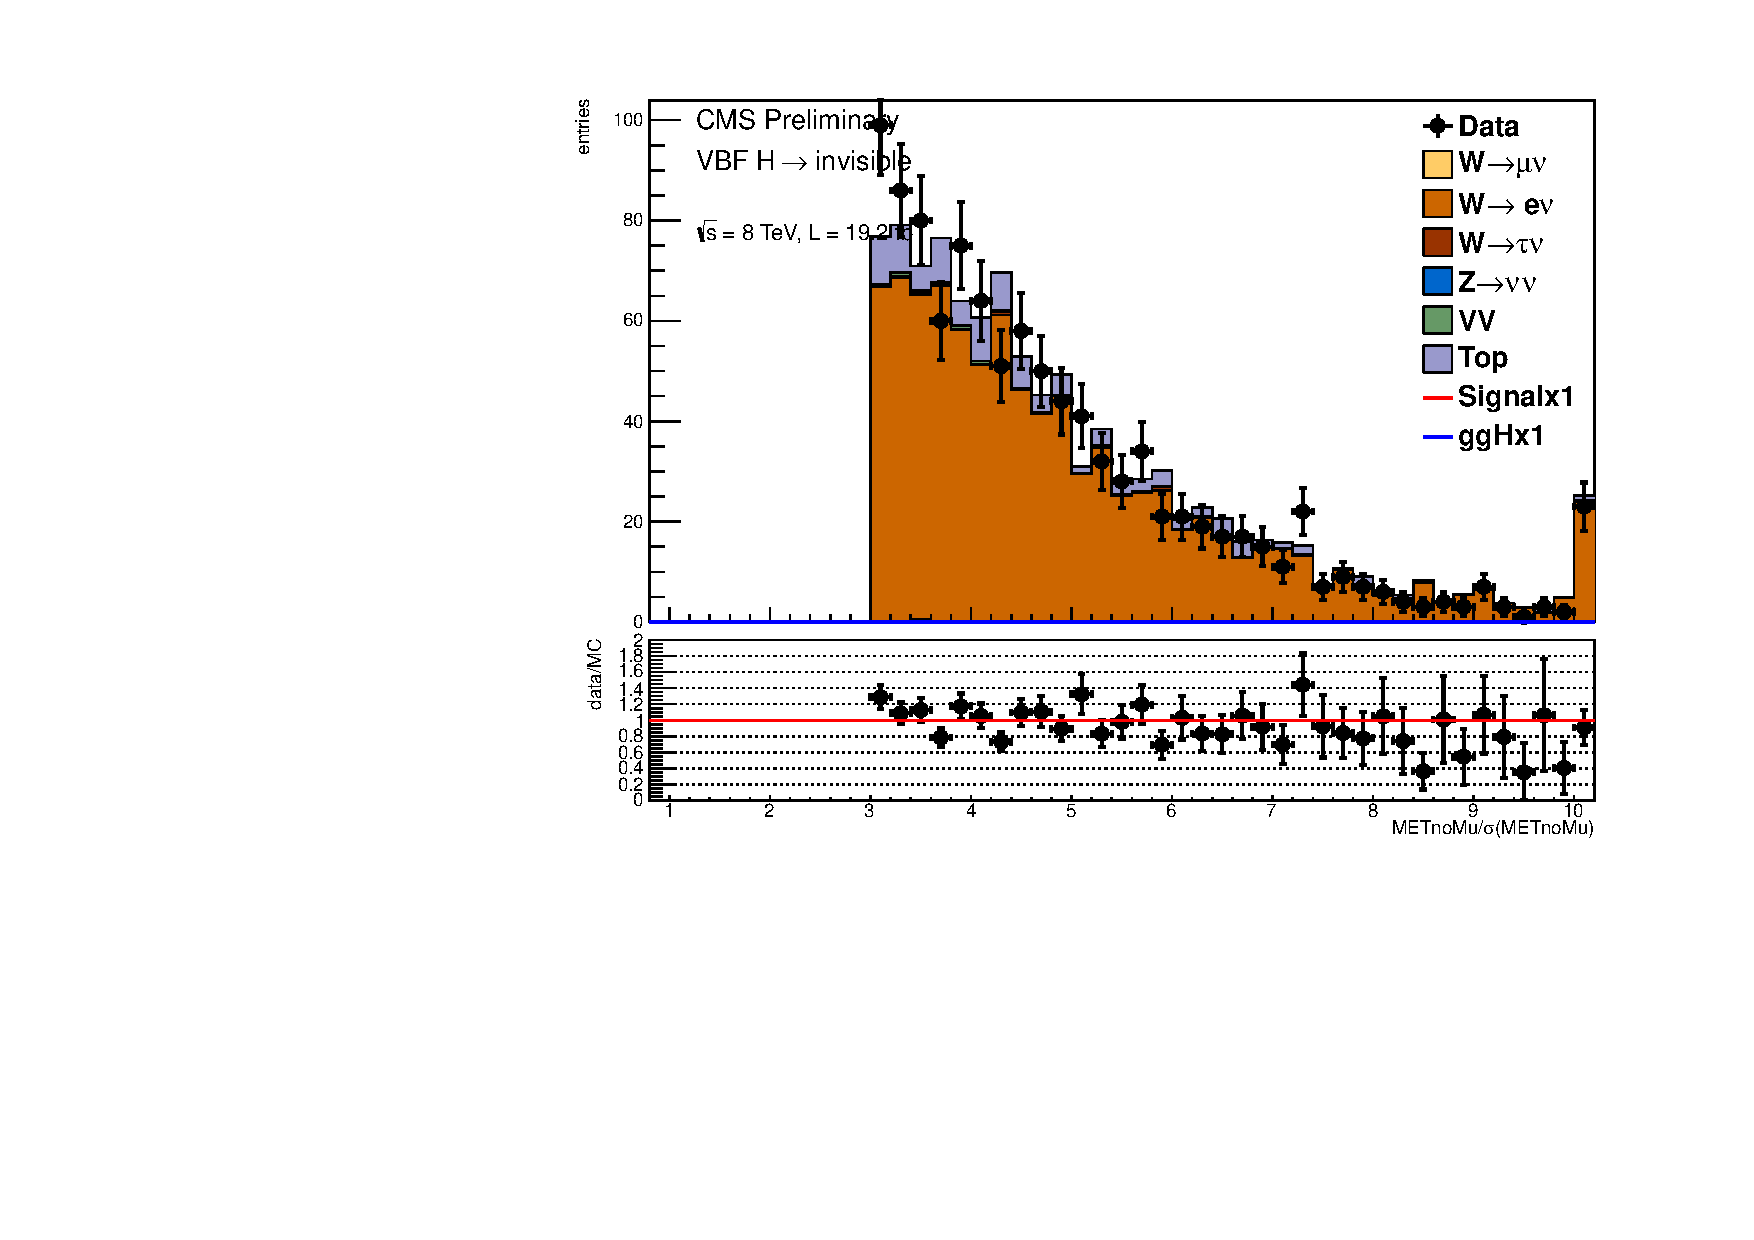
\includegraphics[width=\textwidth]{TalkPics/runcbug101114/output_presel/enu_metnomu_significance.pdf}
    \end{block}

  \end{columns}
\end{frame}

\begin{frame}
  \frametitle{New control plots - enu}
  \begin{columns}
    \column{.5\textwidth}
    \begin{block}{Mjj}
      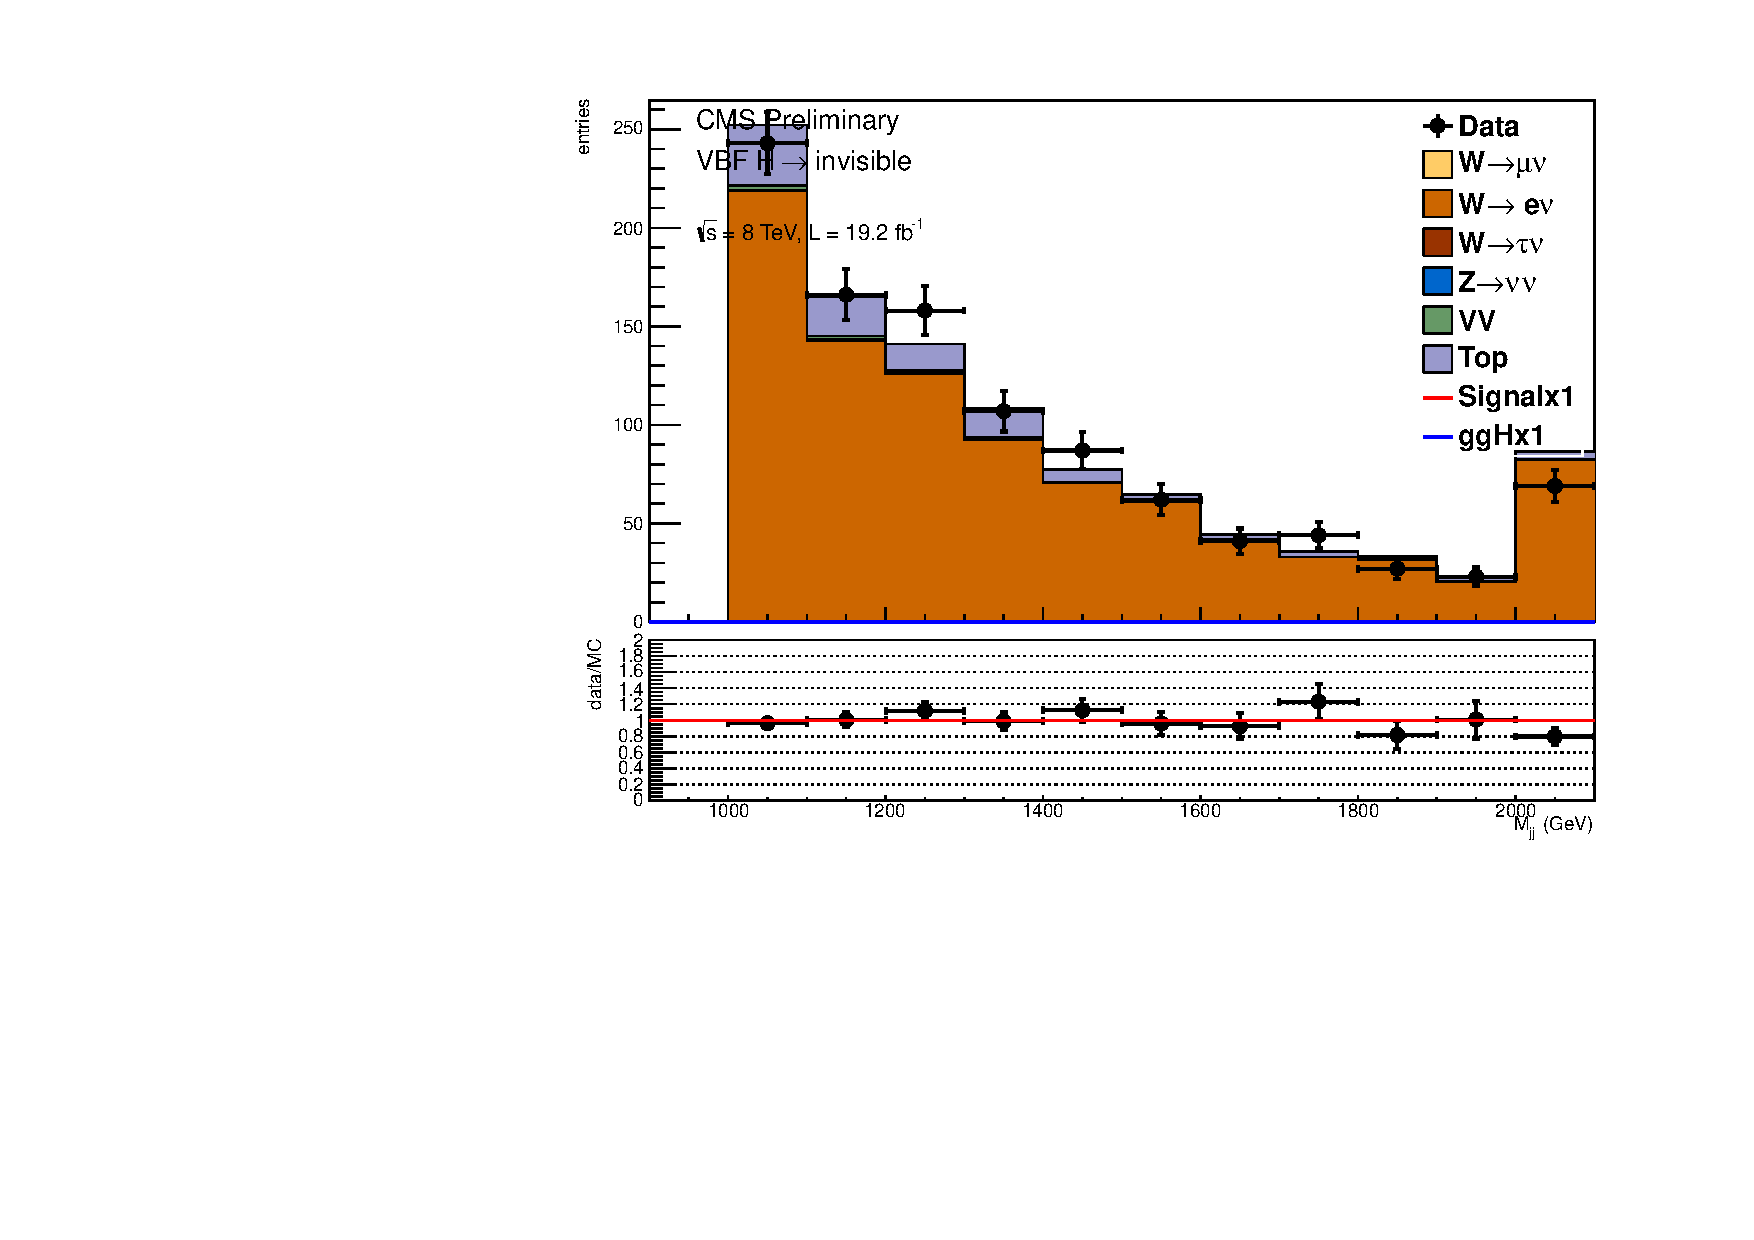
\includegraphics[width=\textwidth]{TalkPics/runcbug101114/output_presel/enu_dijet_M.pdf}
    \end{block}
    \column{.5\textwidth}
    \begin{block}{mt}
      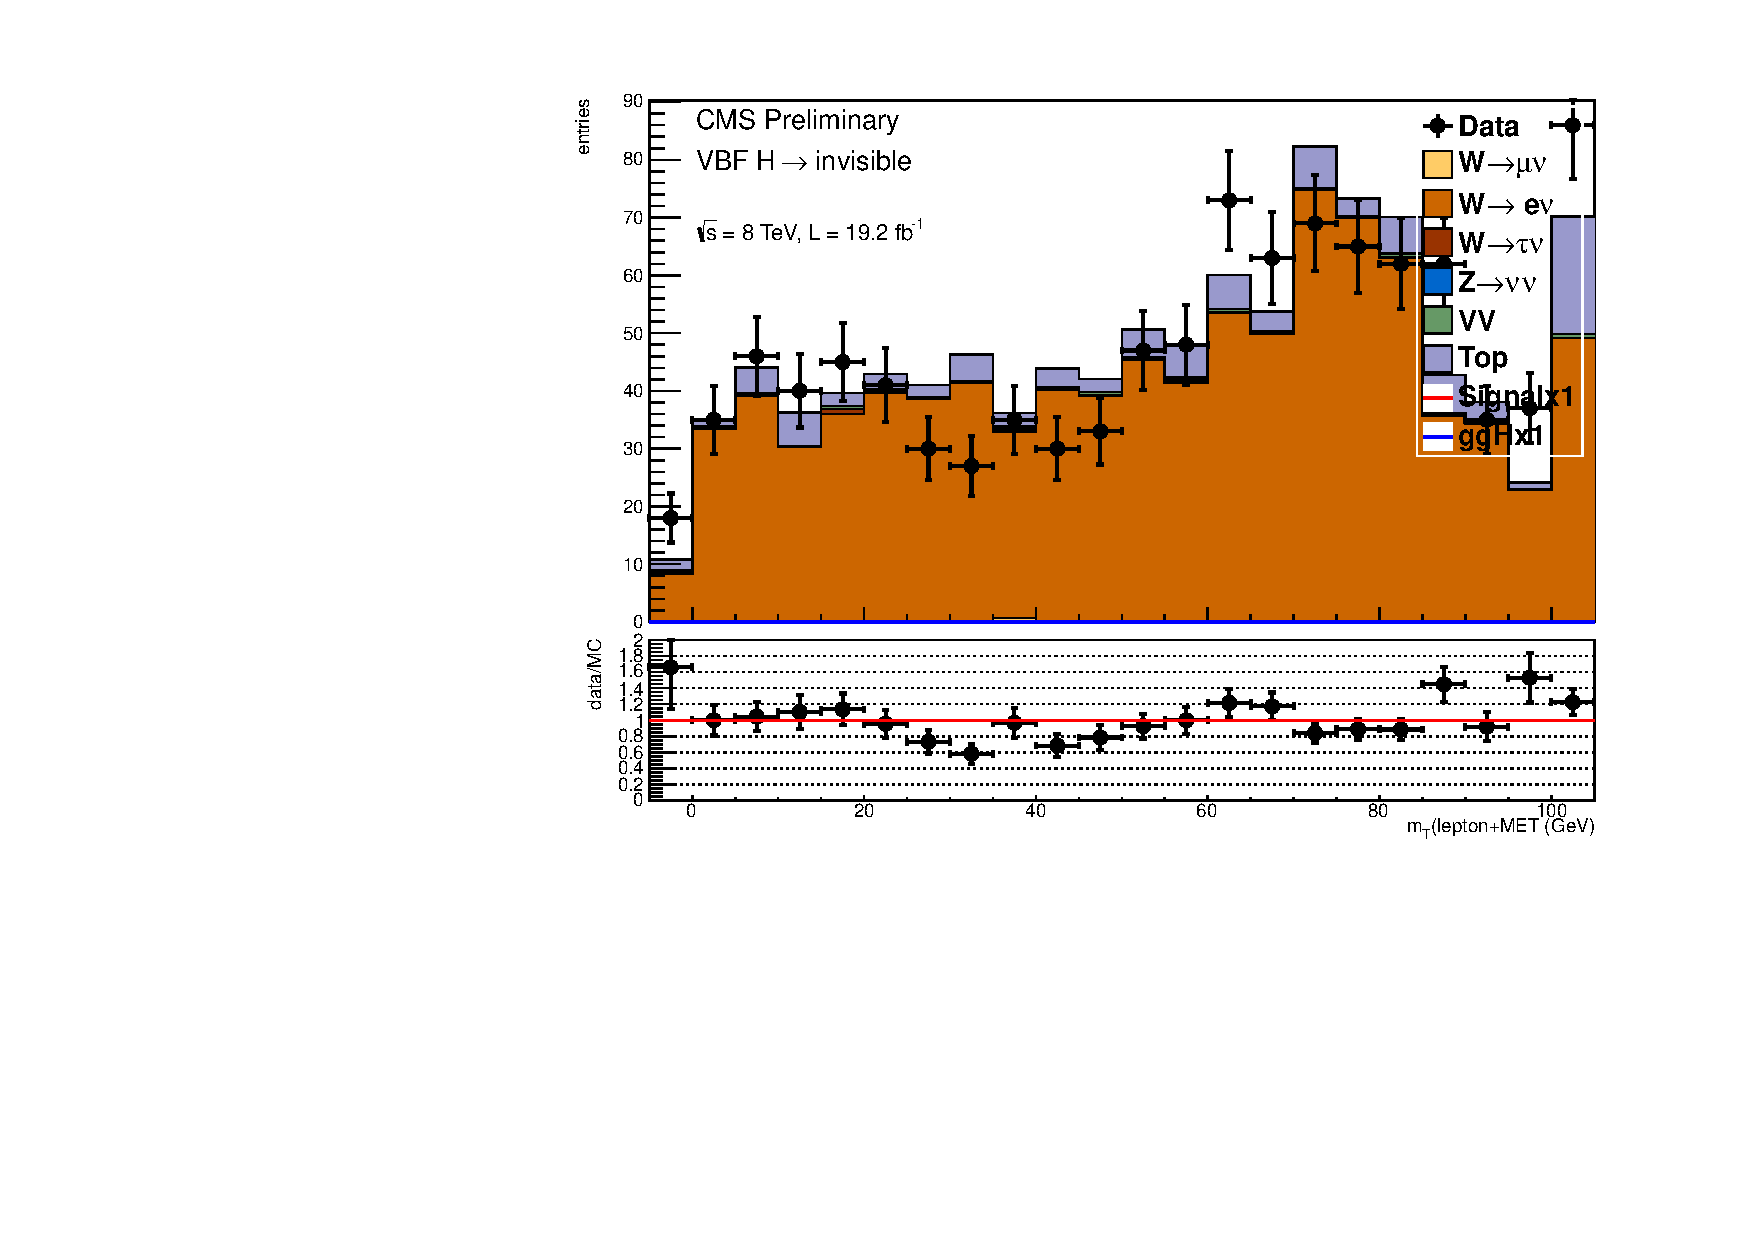
\includegraphics[width=\textwidth]{TalkPics/runcbug101114/output_presel/enu_lep_mt.pdf}
    \end{block}
  \end{columns}
\end{frame}

\begin{frame}
  \frametitle{New control plots - enu}
  \begin{columns}
    \column{.5\textwidth}
    \begin{block}{Dijet Dphi}
      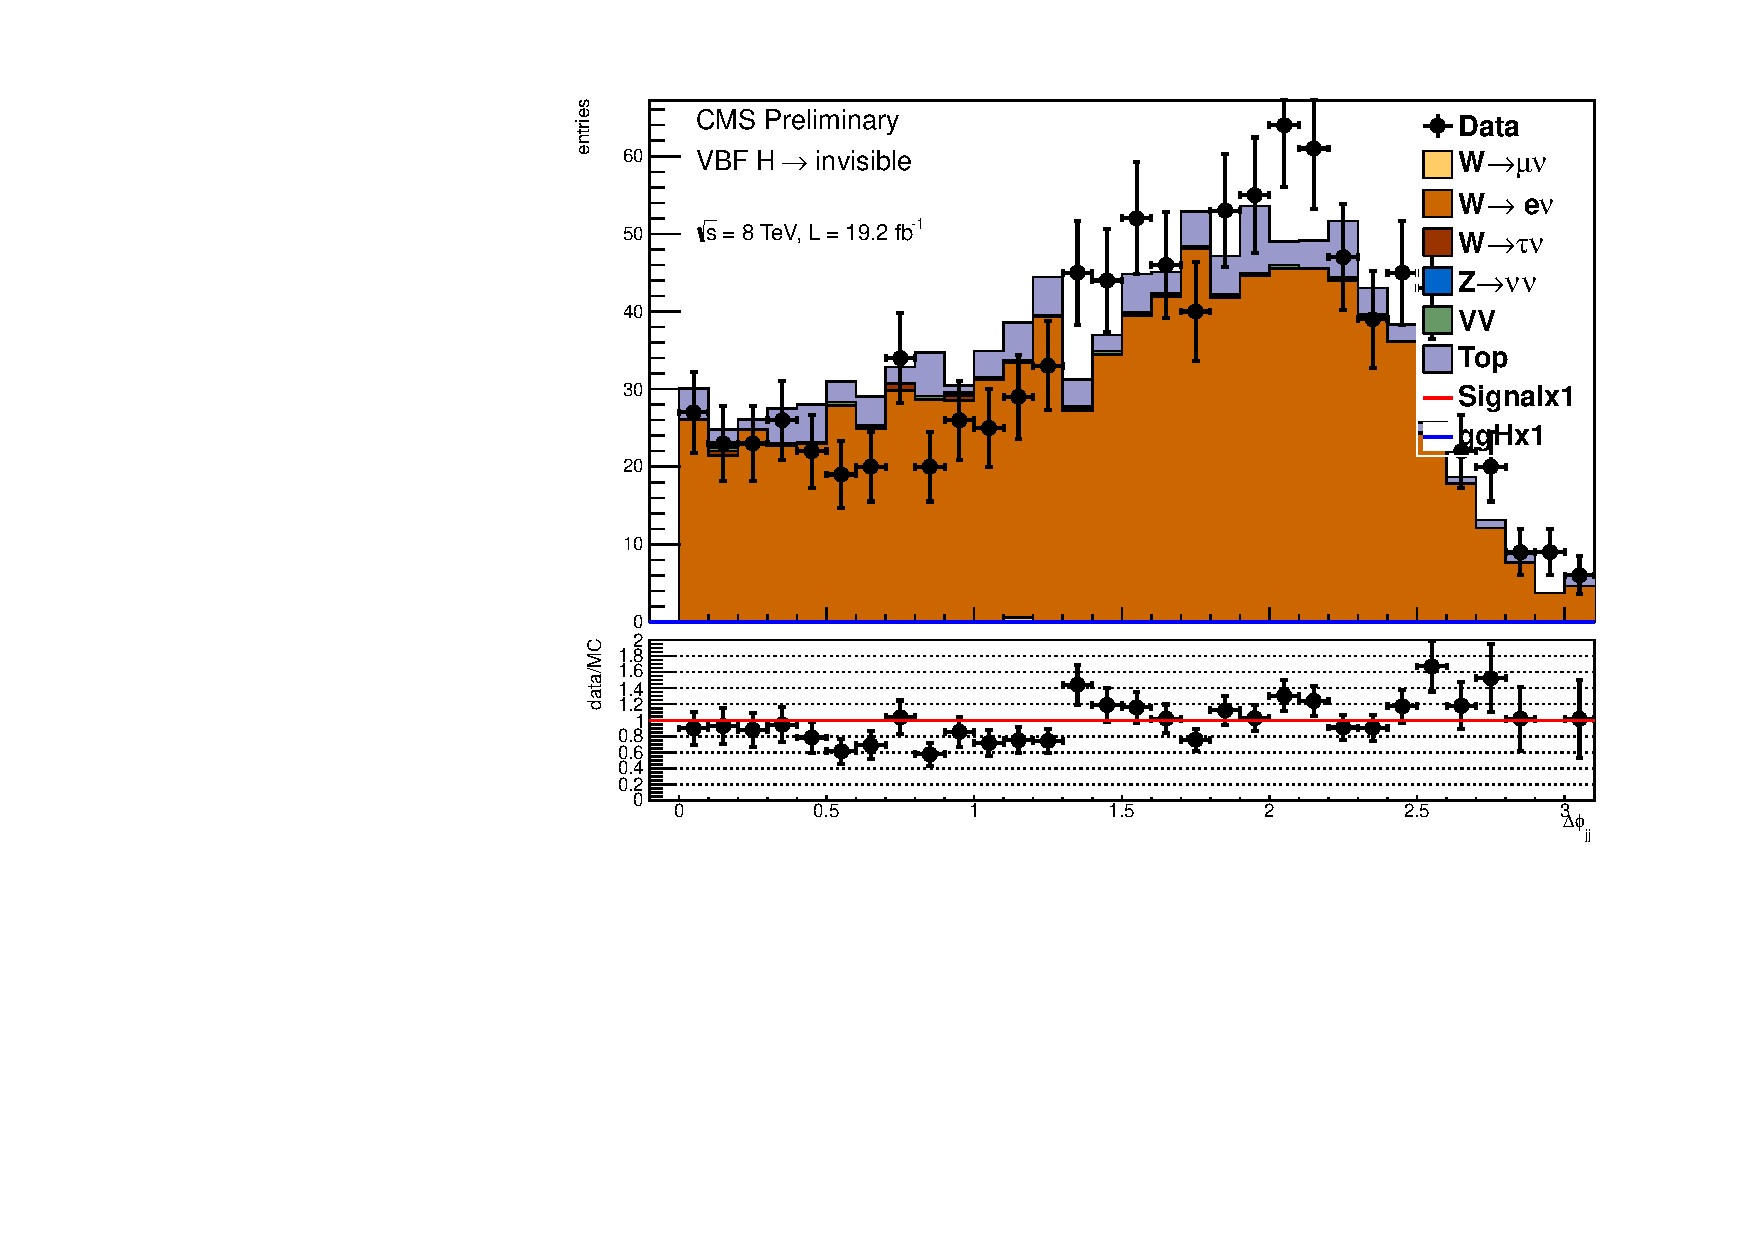
\includegraphics[width=\textwidth]{TalkPics/runcbug101114/output_presel/enu_dijet_dphi.pdf}
    \end{block}
    \column{.5\textwidth}
    \begin{block}{Detajj}
      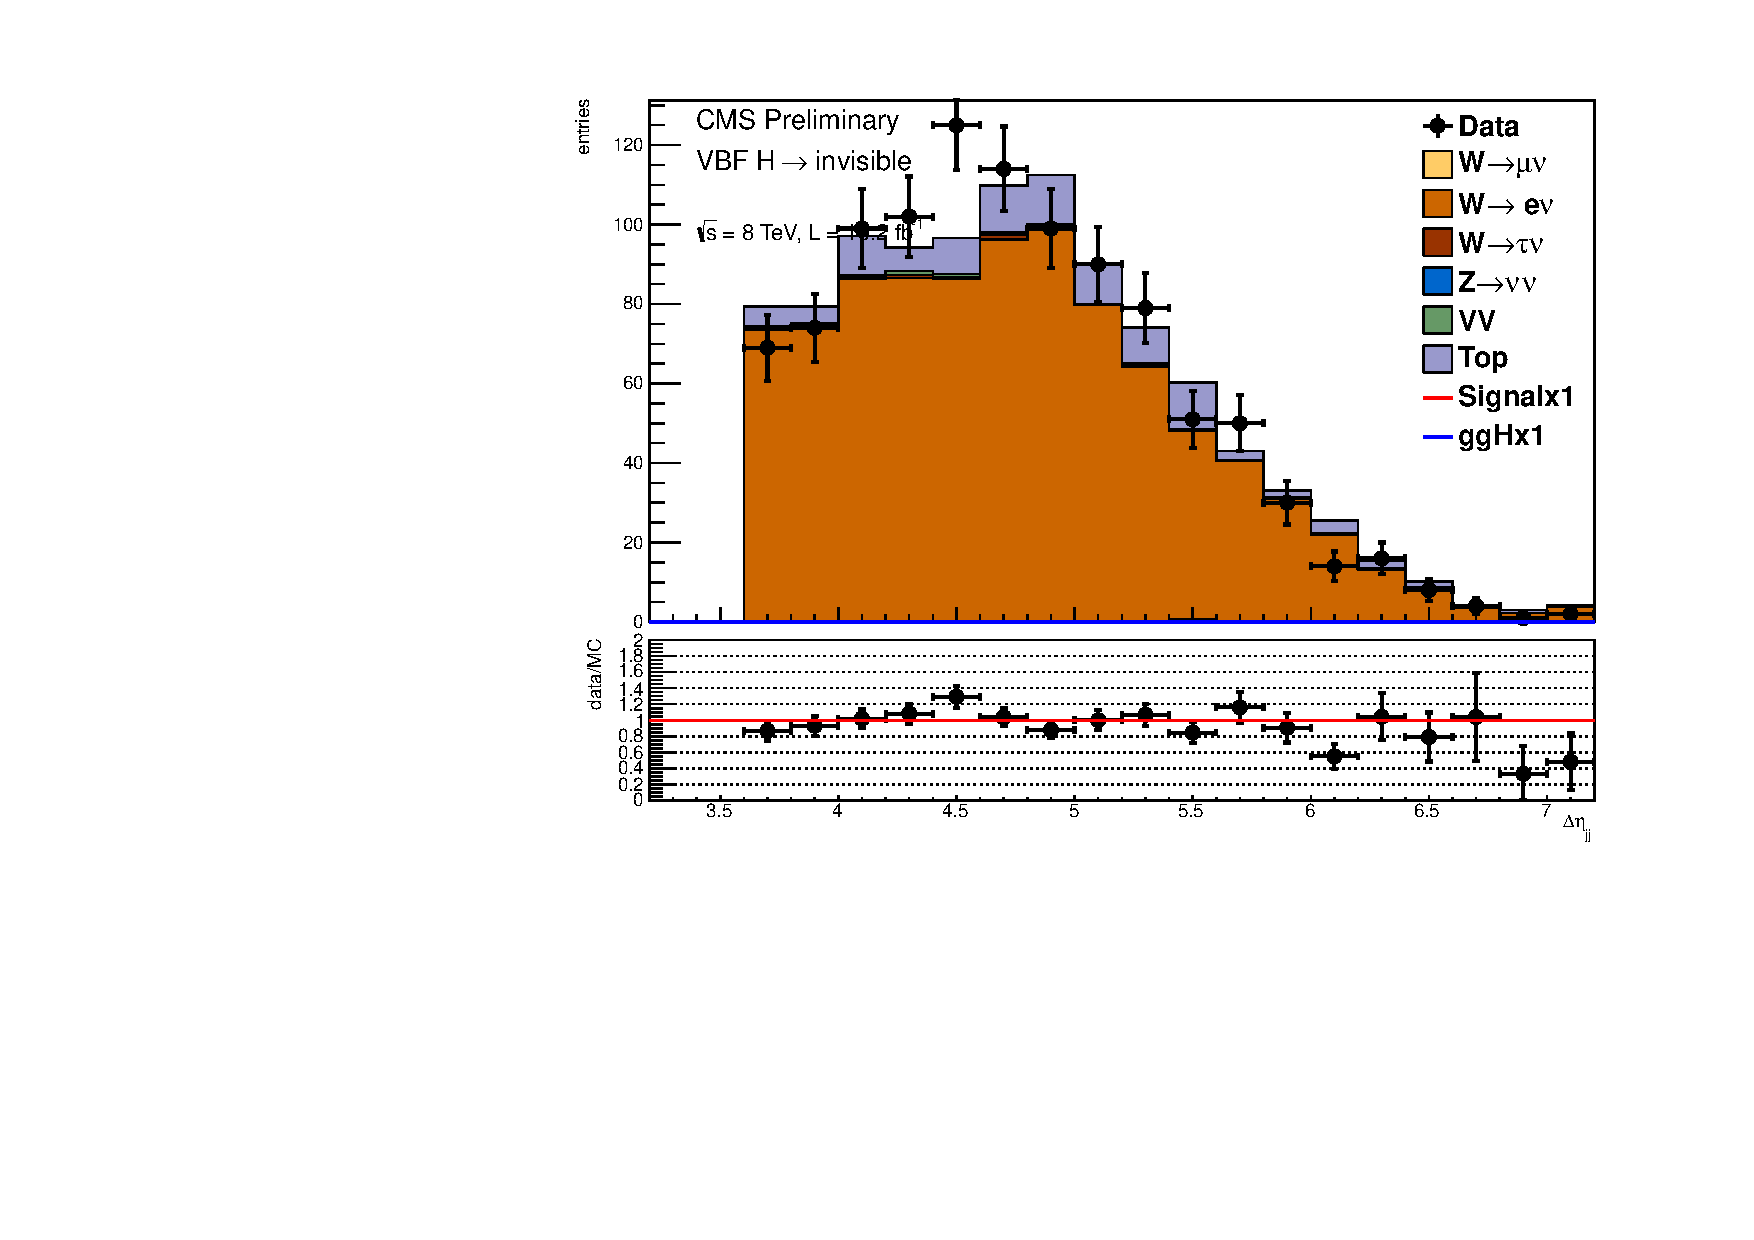
\includegraphics[width=\textwidth]{TalkPics/runcbug101114/output_presel/enu_dijet_deta.pdf}
    \end{block}

  \end{columns}
\end{frame}

\begin{frame}
  \frametitle{New control plots - enu}
  \begin{columns}
    \column{.5\textwidth}
    \begin{block}{Leading jets-met mindphi}
      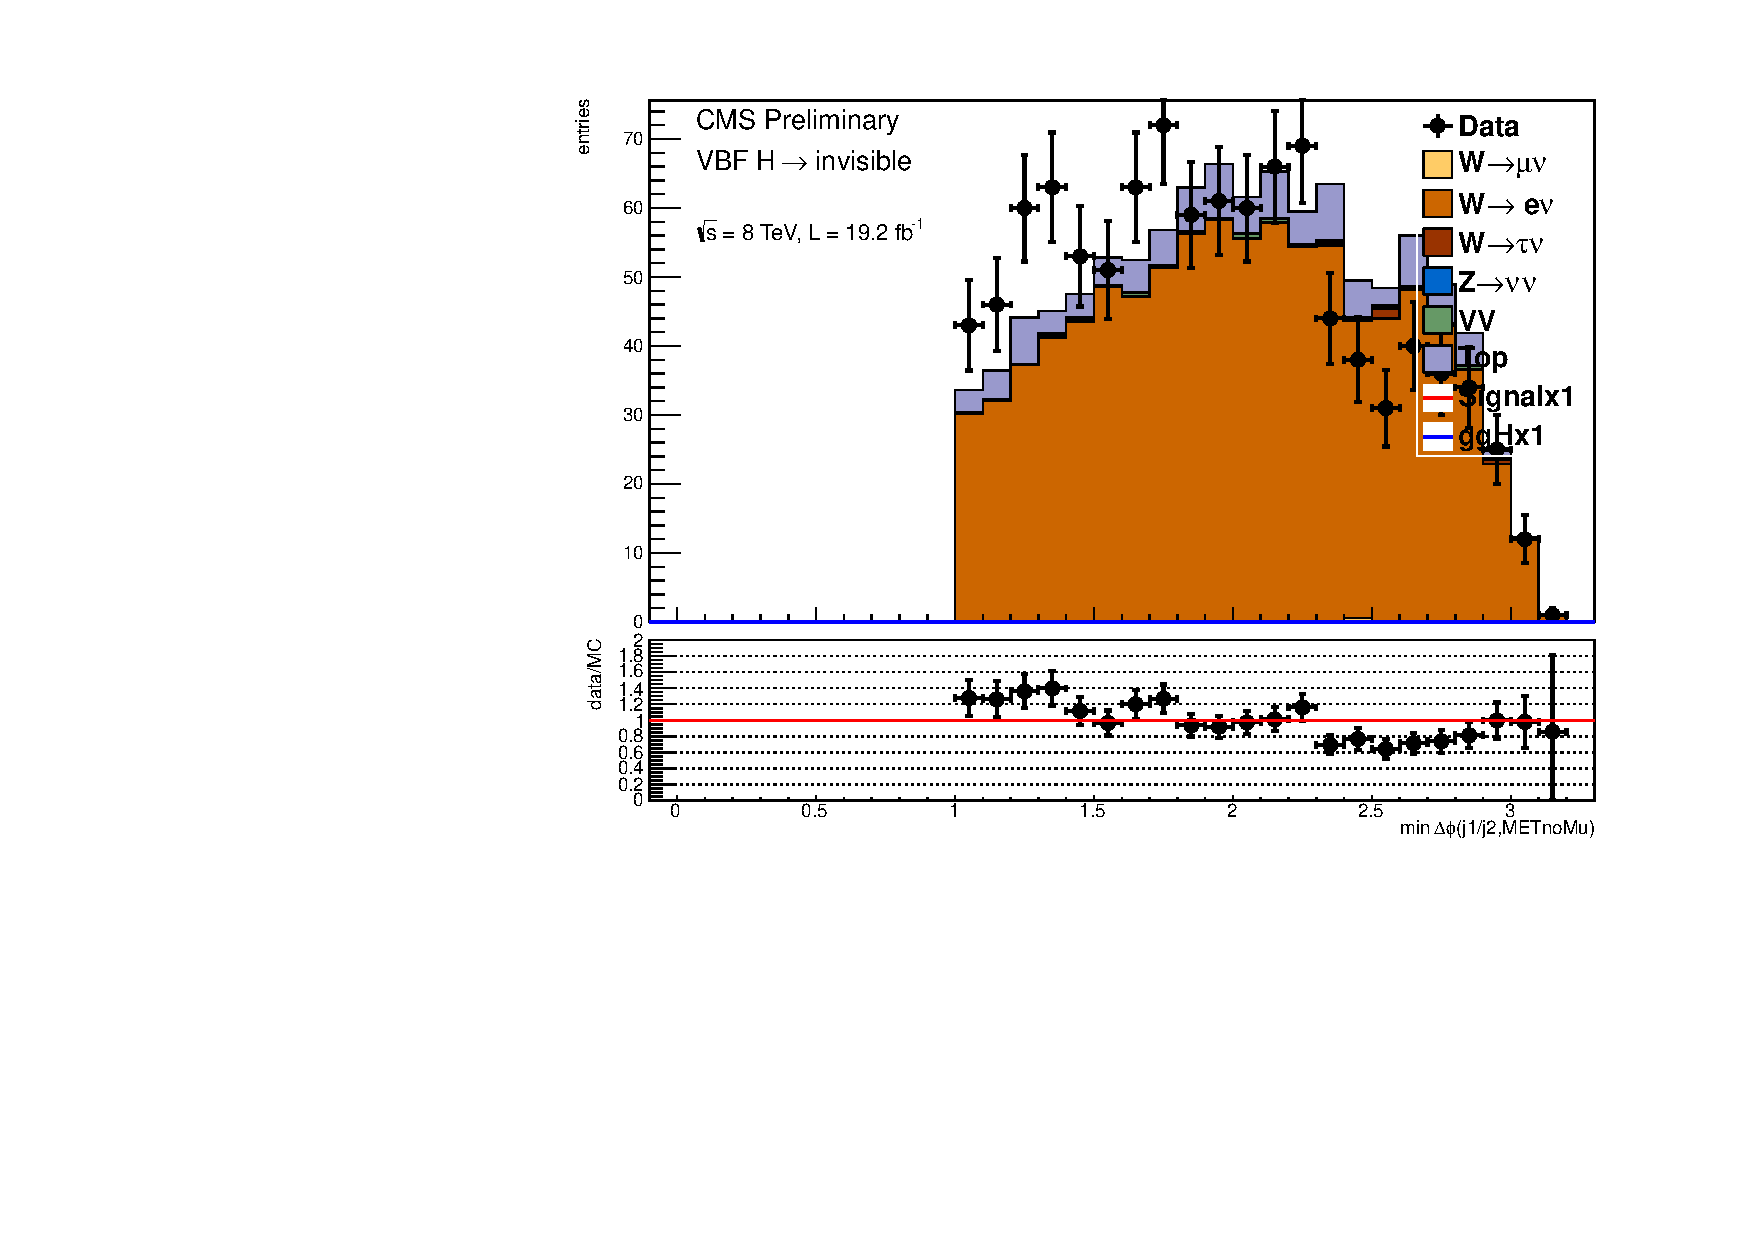
\includegraphics[width=\textwidth]{TalkPics/runcbug101114/output_presel/enu_jetmetnomu_mindphi.pdf}
    \end{block}
    \column{.5\textwidth}
    \begin{block}{All jets-met mindphi}
      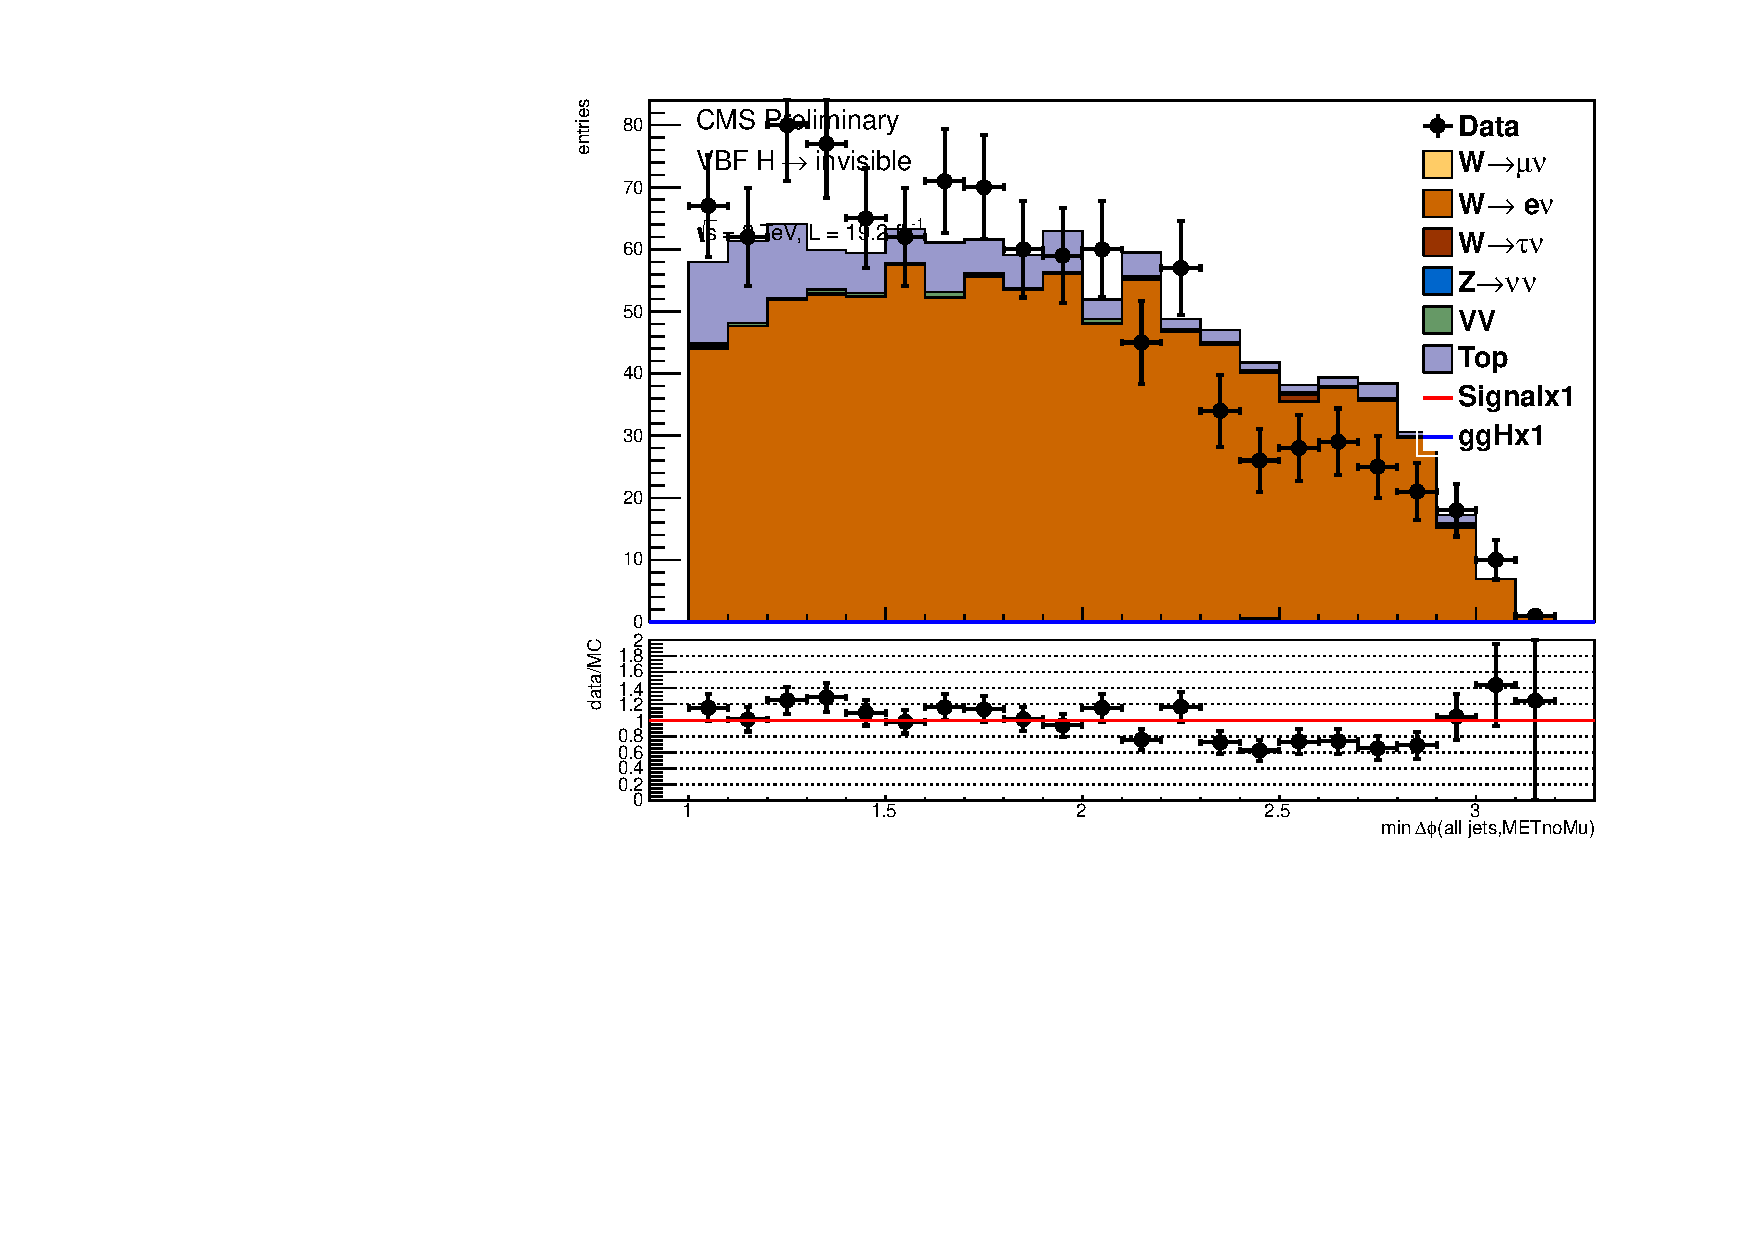
\includegraphics[width=\textwidth]{TalkPics/runcbug101114/output_presel/enu_alljetsmetnomu_mindphi.pdf}
    \end{block}

  \end{columns}
\end{frame}

\begin{frame}
  \frametitle{New control plots - enu}
  \begin{columns}
    \column{.5\textwidth}
    \begin{block}{dijet-metnomu pt fraction}
      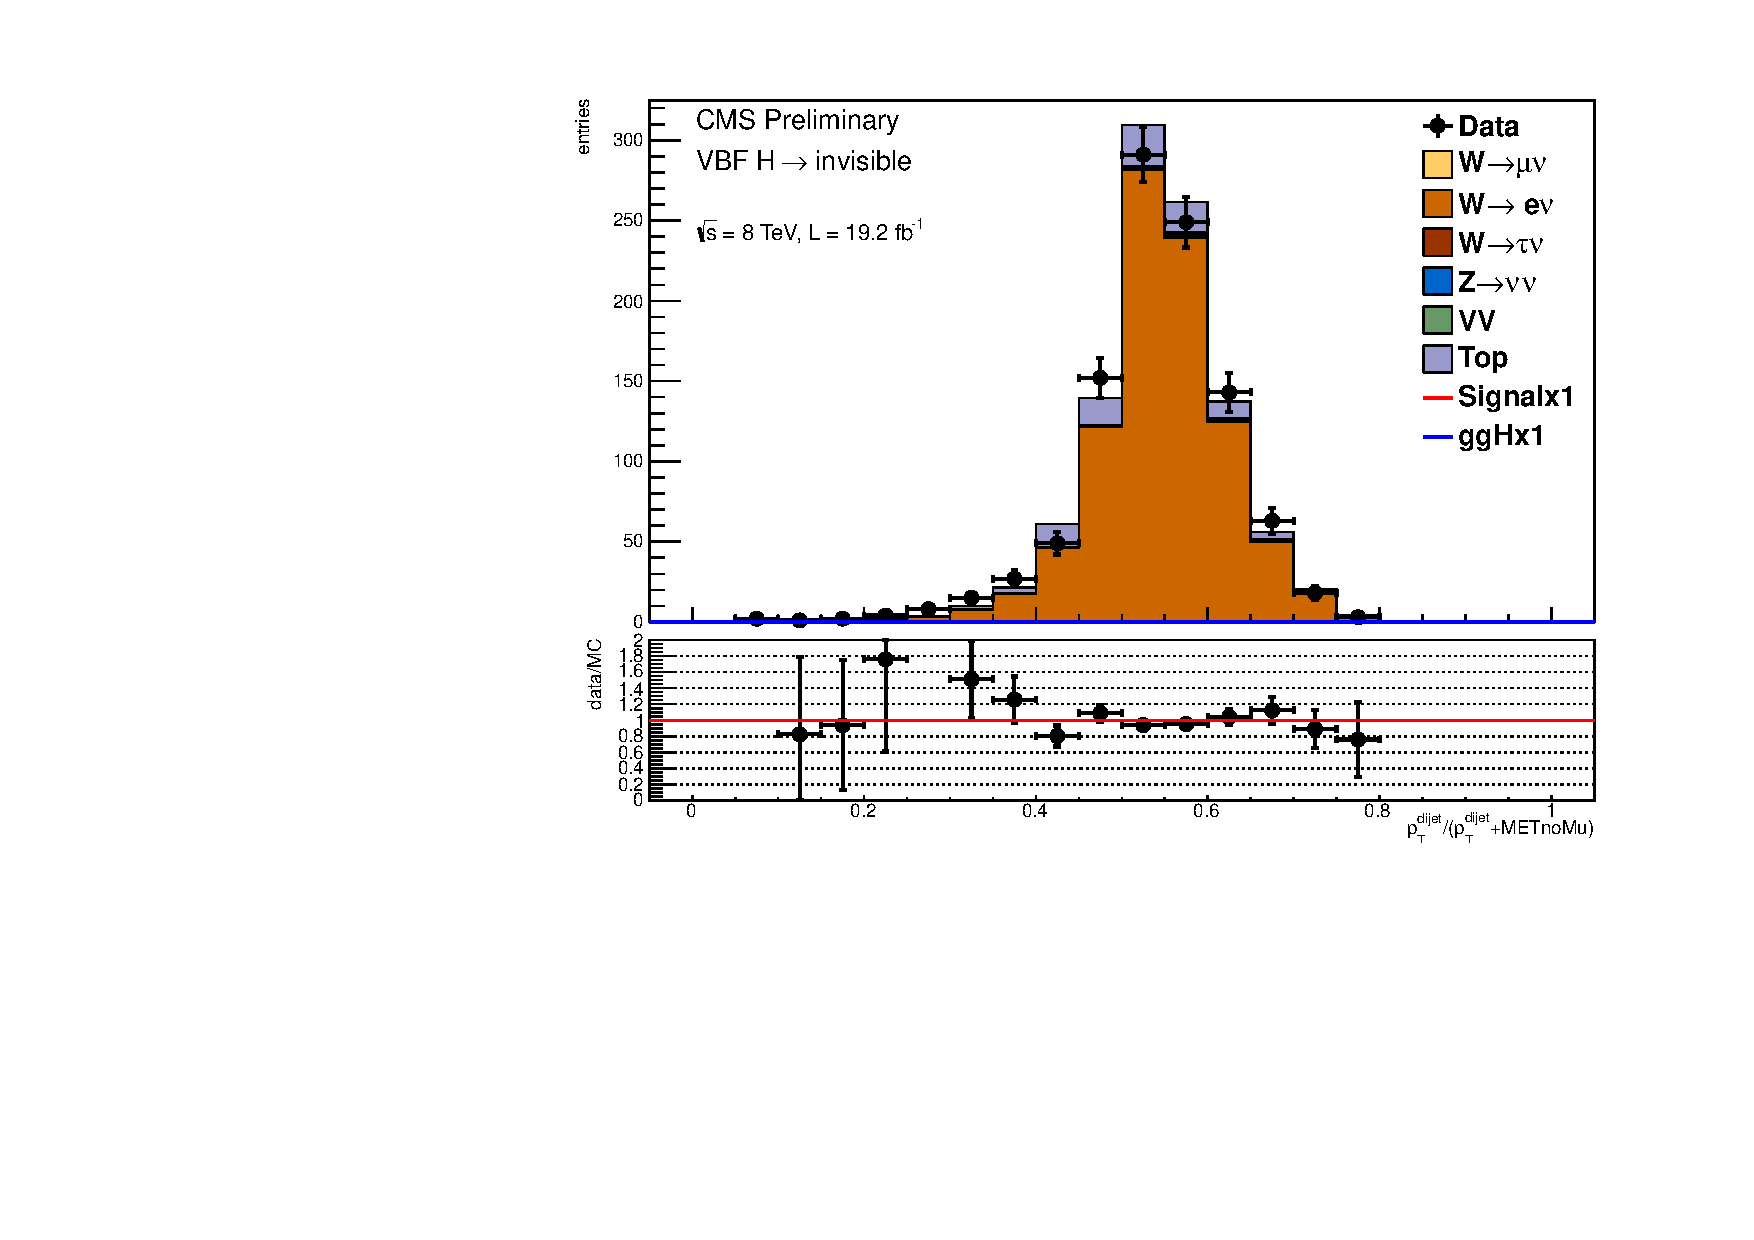
\includegraphics[width=\textwidth]{TalkPics/runcbug101114/output_presel/enu_dijetmetnomu_ptfraction.pdf}
    \end{block}
  \end{columns}
\end{frame}

\begin{frame}
  \frametitle{New control plots - munu}
  \begin{columns}
    \column{.5\textwidth}
    \begin{block}{Jet 1 pt}
      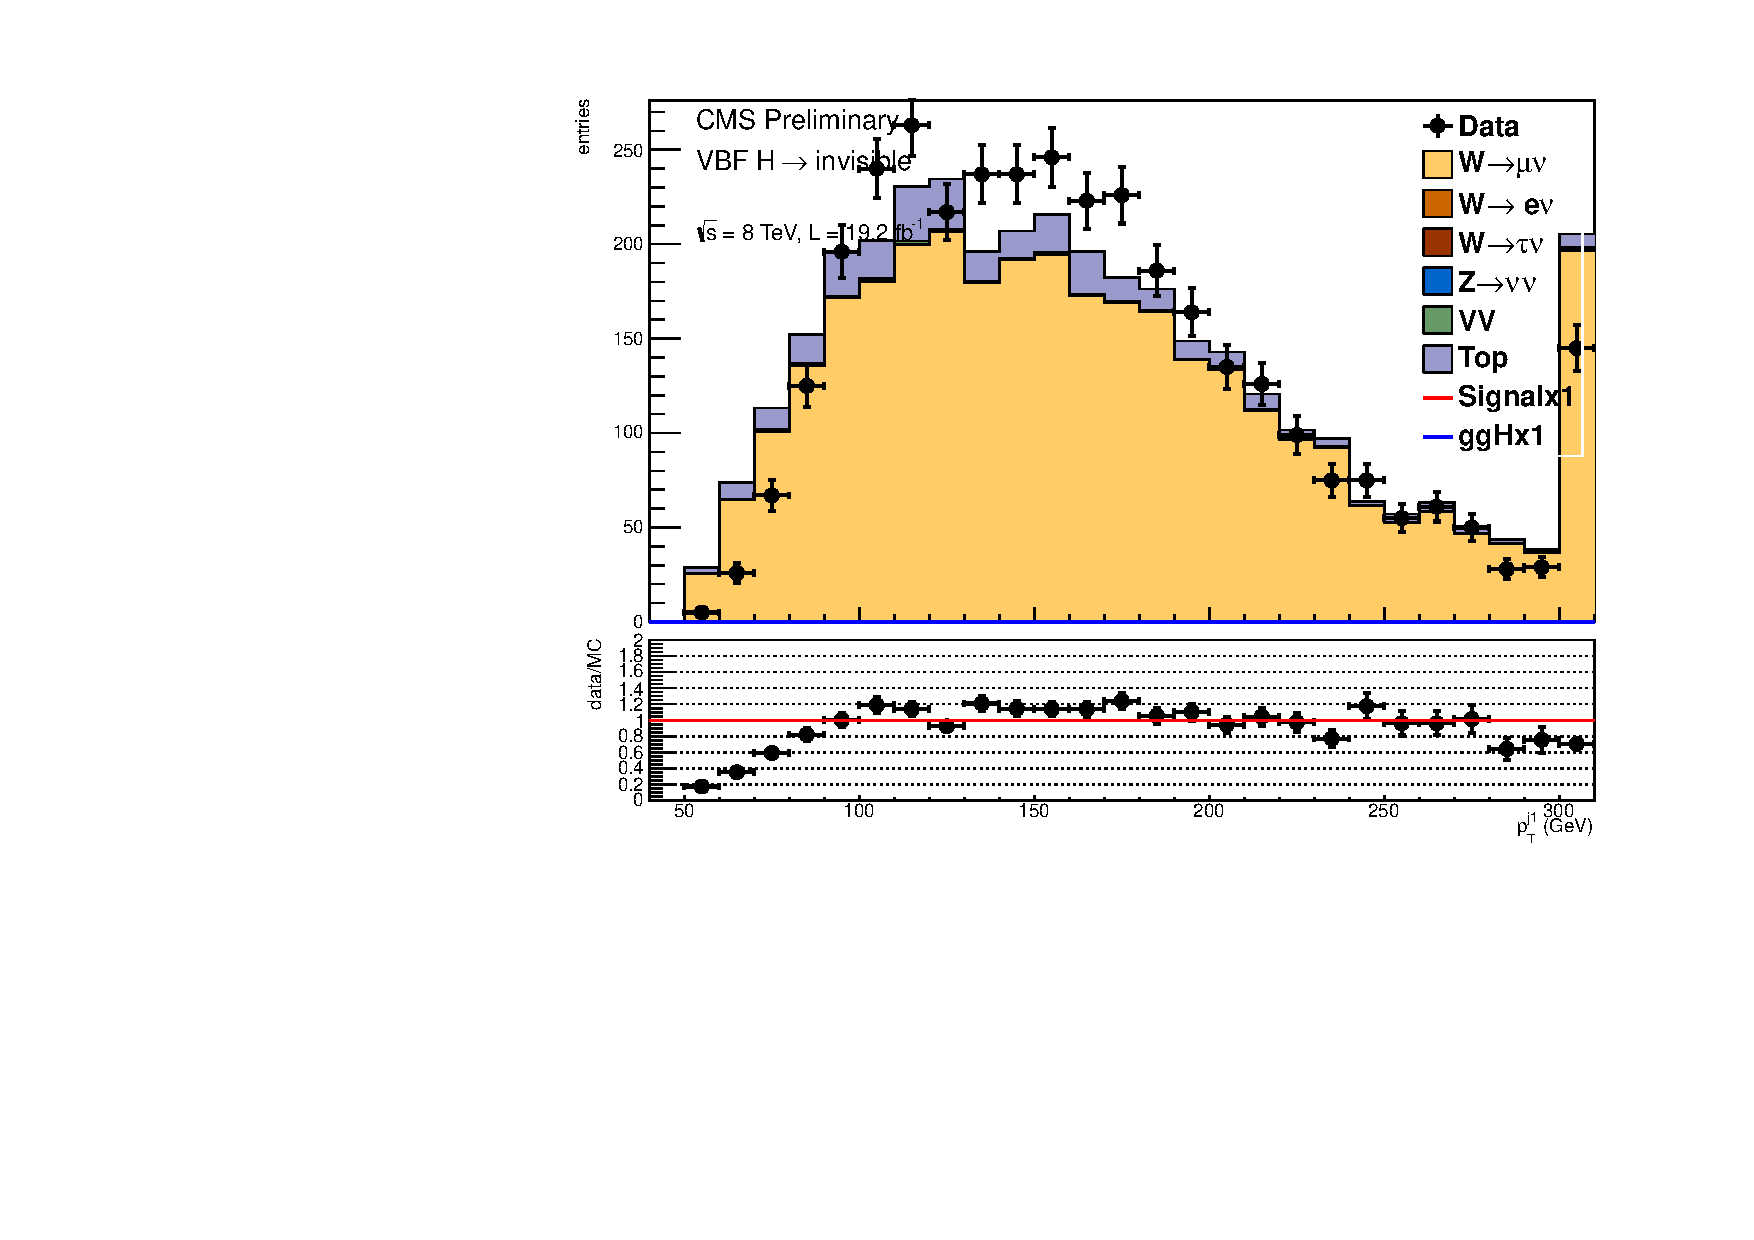
\includegraphics[width=\textwidth]{TalkPics/runcbug101114/output_presel/munu_jet1_pt.pdf}
    \end{block}
    \column{.5\textwidth}
    \begin{block}{Jet 2 pt}
      \includegraphics[width=\textwidth]{TalkPics/runcbug101114/output_presel/munu_jet2_pt.pdf}
    \end{block}

  \end{columns}
\end{frame}

\begin{frame}
  \frametitle{New control plots - munu}
  \begin{columns}
    \column{.5\textwidth}
    \begin{block}{METnomu}
      \includegraphics[width=\textwidth]{TalkPics/runcbug101114/output_presel/munu_metnomuons.pdf}
    \end{block}
    \column{.5\textwidth}
    \begin{block}{METnomusig}
      \includegraphics[width=\textwidth]{TalkPics/runcbug101114/output_presel/munu_metnomu_significance.pdf}
    \end{block}

  \end{columns}
\end{frame}

\begin{frame}
  \frametitle{New control plots - munu}
  \begin{columns}
    \column{.5\textwidth}
    \begin{block}{Mjj}
      \includegraphics[width=\textwidth]{TalkPics/runcbug101114/output_presel/munu_dijet_M.pdf}
    \end{block}
    \column{.5\textwidth}
    \begin{block}{mt}
      \includegraphics[width=\textwidth]{TalkPics/runcbug101114/output_presel/munu_lep_mt.pdf}
    \end{block}
  \end{columns}
\end{frame}

\begin{frame}
  \frametitle{New control plots - munu}
  \begin{columns}
    \column{.5\textwidth}
    \begin{block}{Dijet Dphi}
      \includegraphics[width=\textwidth]{TalkPics/runcbug101114/output_presel/munu_dijet_dphi.pdf}
    \end{block}
    \column{.5\textwidth}
    \begin{block}{Detajj}
      \includegraphics[width=\textwidth]{TalkPics/runcbug101114/output_presel/munu_dijet_deta.pdf}
    \end{block}

  \end{columns}
\end{frame}

\begin{frame}
  \frametitle{New control plots - munu}
  \begin{columns}
    \column{.5\textwidth}
    \begin{block}{Leading jets-met mindphi}
      \includegraphics[width=\textwidth]{TalkPics/runcbug101114/output_presel/munu_jetmetnomu_mindphi.pdf}
    \end{block}
    \column{.5\textwidth}
    \begin{block}{All jets-met mindphi}
      \includegraphics[width=\textwidth]{TalkPics/runcbug101114/output_presel/munu_alljetsmetnomu_mindphi.pdf}
    \end{block}

  \end{columns}
\end{frame}

\begin{frame}
  \frametitle{New control plots - munu}
  \begin{columns}
    \column{.5\textwidth}
    \begin{block}{dijet-metnomu pt fraction}
      \includegraphics[width=\textwidth]{TalkPics/runcbug101114/output_presel/munu_dijetmetnomu_ptfraction.pdf}
    \end{block}
  \end{columns}
\end{frame}

\begin{frame}
  \frametitle{New control plots - taunu}
  \begin{columns}
    \column{.5\textwidth}
    \begin{block}{Jet 1 pt}
      \includegraphics[width=\textwidth]{TalkPics/runcbug101114/output_presel/taunu_jet1_pt.pdf}
    \end{block}
    \column{.5\textwidth}
    \begin{block}{Jet 2 pt}
      \includegraphics[width=\textwidth]{TalkPics/runcbug101114/output_presel/taunu_jet2_pt.pdf}
    \end{block}

  \end{columns}
\end{frame}

\begin{frame}
  \frametitle{New control plots - taunu}
  \begin{columns}
    \column{.5\textwidth}
    \begin{block}{METnomu}
      \includegraphics[width=\textwidth]{TalkPics/runcbug101114/output_presel/taunu_metnomuons.pdf}
    \end{block}
    \column{.5\textwidth}
    \begin{block}{METnomusig}
      \includegraphics[width=\textwidth]{TalkPics/runcbug101114/output_presel/taunu_metnomu_significance.pdf}
    \end{block}

  \end{columns}
\end{frame}

\begin{frame}
  \frametitle{New control plots - taunu}
  \begin{columns}
    \column{.5\textwidth}
    \begin{block}{Mjj}
      \includegraphics[width=\textwidth]{TalkPics/runcbug101114/output_presel/taunu_dijet_M.pdf}
    \end{block}
    \column{.5\textwidth}
    \begin{block}{mt}
      \includegraphics[width=\textwidth]{TalkPics/runcbug101114/output_presel/taunu_lep_mt.pdf}
    \end{block}
  \end{columns}
\end{frame}

\begin{frame}
  \frametitle{New control plots - taunu}
  \begin{columns}
    \column{.5\textwidth}
    \begin{block}{Dijet Dphi}
      \includegraphics[width=\textwidth]{TalkPics/runcbug101114/output_presel/taunu_dijet_dphi.pdf}
    \end{block}
    \column{.5\textwidth}
    \begin{block}{Detajj}
      \includegraphics[width=\textwidth]{TalkPics/runcbug101114/output_presel/taunu_dijet_deta.pdf}
    \end{block}

  \end{columns}
\end{frame}

\begin{frame}
  \frametitle{New control plots - taunu}
  \begin{columns}
    \column{.5\textwidth}
    \begin{block}{Leading jets-met mindphi}
      \includegraphics[width=\textwidth]{TalkPics/runcbug101114/output_presel/taunu_jetmetnomu_mindphi.pdf}
    \end{block}
    \column{.5\textwidth}
    \begin{block}{All jets-met mindphi}
      \includegraphics[width=\textwidth]{TalkPics/runcbug101114/output_presel/taunu_alljetsmetnomu_mindphi.pdf}
    \end{block}

  \end{columns}
\end{frame}

\begin{frame}
  \frametitle{New control plots - taunu}
  \begin{columns}
    \column{.5\textwidth}
    \begin{block}{dijet-metnomu pt fraction}
      \includegraphics[width=\textwidth]{TalkPics/runcbug101114/output_presel/taunu_dijetmetnomu_ptfraction.pdf}
    \end{block}
  \end{columns}
\end{frame}

\end{fmffile}
\end{document}
